\chapter{Background estimation}
\label{chap:backgrounds}

There are three main classes of backgrounds that survive the inclusive SUSY or
\smft analysis baseline selections: backgrounds with two or more prompt leptons
in the final state (giving a real SS pair), backgrounds with at least one nonprompt lepton,
and backgrounds that actually have an OS pair with one lepton having misreconstructed charge.

The first class of backgrounds produce prompt leptons
but are relatively ``rare'' (have low cross section) and are estimated from
simulation, with appropriate correction factors and uncertainties to be discussed in the next
sections. This class can be further subdivided by the physical process:

\begin{itemize}
    \item \textbf{Diboson}: \\ \WZ, \ZZ, \WW, \WH, \ZH, \Zgamma, \Wgamma, and \WpWp
    \item \textbf{Triboson}: \\ \WWW, \WWZ, \WZZ, \ZZZ, \WWgamma, and \WZgamma
    \item \textbf{Single top quark and bosons}: \\ \tgamma, \tZgamma, and \tWZ
    \item \textbf{Top quark pair and one boson}: \\ \ttW, \ttZ, \ttH, and \ttgamma
    \item \textbf{Top quark pair and two bosons}: \\ \ttWW, \ttWZ, \ttZZ, \ttWH, \ttZH, and \ttHH
    \item \textbf{Triple top quark}: \\ \ttt and \tttW
    \item \textbf{Four top quarks}: \\ \tttt
\end{itemize}

In the \smft analysis, \tttt is, of course, considered a signal instead of a background.
Contributions from the first two categories of physical processes are negligible for the
\smft analysis due to the $\Nbjets\geq 2$ requirement in the baseline selections.

The second class of background events consist of events where one of the leptons is
``nonprompt'', or more colloquially, ``fake''. That is, the fake lepton is
either a real lepton which is a decay product of a heavy flavor hadron (\PQb 
or \PQc quark), or simply a misidentified hadron. The dominant sources of fake leptons
are the large cross section processes of $\ttjets$ and $\wjets$. This class is more
tricky to only use simulation, and a data-driven method is used instead.

The last class of backgrounds consists of those with a charge-misidentified lepton, or,
more colloquially ``flips'', which essentially
converts an OS pair into a SS pair. Thus, the biggest source of this background is 
the highest cross-section OS process: DY. Similarly to
the nonprompt background, this background uses a data-driven method instead of 
relying completely on simulation.

\section{Prompt SM}

The large set of physics processes listed in the previous section as prompt SM processes
are estimated from simulation and are grouped into larger categories, singling out
specific processes which are important to either  the inclusive SUSY analysis
or the \smft analysis. The process categories and constitutent physics processes/simulations
are:

\begin{itemize}
    \item ``$\mathbf{\ttW}$'': \ttW
    \item ``$\mathbf{\ttZ}$'': \ttZ
    \item ``$\mathbf{\ttH}$'': \ttH
    \item ``$\mathbf{\Xgamma}$'': \Wgamma, \Zgamma, \ttgamma, and \tgamma
\end{itemize}

And for the \smft analysis, there are two additional categories:
\begin{itemize}
    \item ``\textbf{Rare}'': \ttt, \tttW, \ZZ, \WH, \ZH, \WZgamma, \WWgamma, \tZgamma, \tWZ, \WpWp, \WZ, and \WW
    \item ``$\mathbf{\ttVV}$'': \ttWW, \ttWZ, \ttZZ, \ttWH, \ttZH, and \ttHH
\end{itemize}

Or, for the inclusive SUSY analysis, there are three additional categories:
\begin{itemize}
    \item ``\textbf{Rare}'': \ttt, \tttW, \ZZ, \WW, \WH, \ZH, \WZgamma, \WWgamma, \tZgamma, \tWZ, \ttWW, \ttWZ, \ttZZ, \ttWH, \ttZH, \ttHH, and \tttt
    \item ``\textbf{WZ}'': \WZ
    \item ``\textbf{WW}'': \WpWp
\end{itemize}

Two important processes for the \smft search are \ttW and \ttZ, which have cross sections
of 630\ifb and 840\ifb~\cite{CMS:Sirunyan2017uzs}, respectively, almost a couple orders of magnitude larger than that of
\tttt (12\ifb).

A breakdown of the individual processes of the ``Rare'' category in the 
\smft analysis signal regions
is shown in Figure~\ref{fig:ftraressr}, split into multi-top quark and multi-boson
processes.

Since many of these processes have not been experimentally observed or measured,
we apply conservative normalization uncertainties based on theoretical calculations of 50\% on
Rare and \Xgamma categories for the SUSY analysis, or 30\% for other categories.

\begin{figure}[!hbtp]
    \centering
    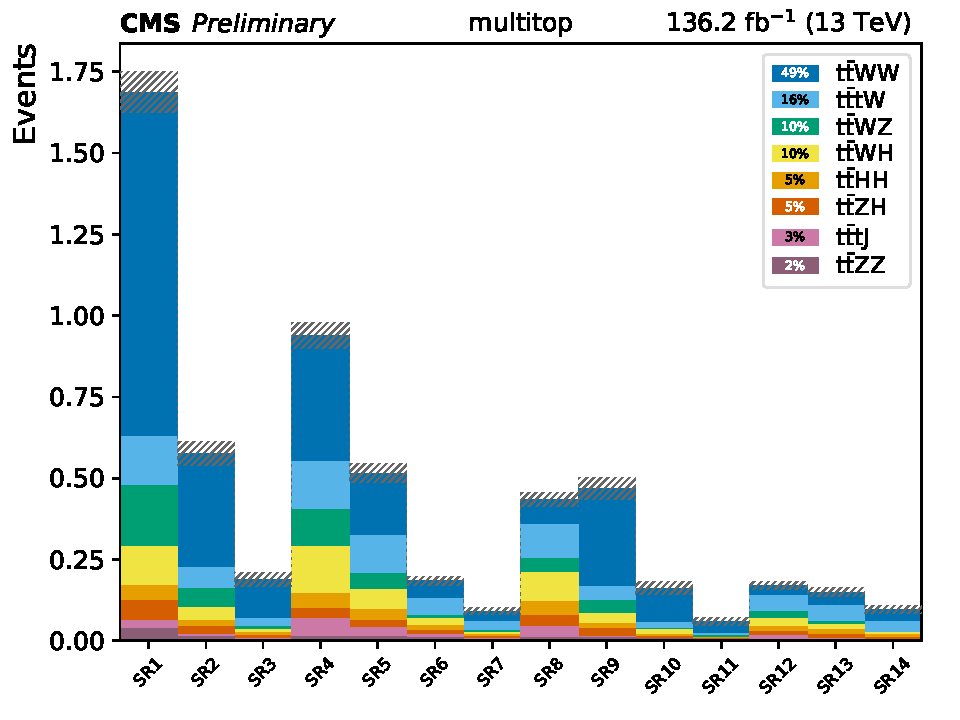
\includegraphics[width=.60\textwidth]{figs/ftan/h_multitop.pdf} \\
    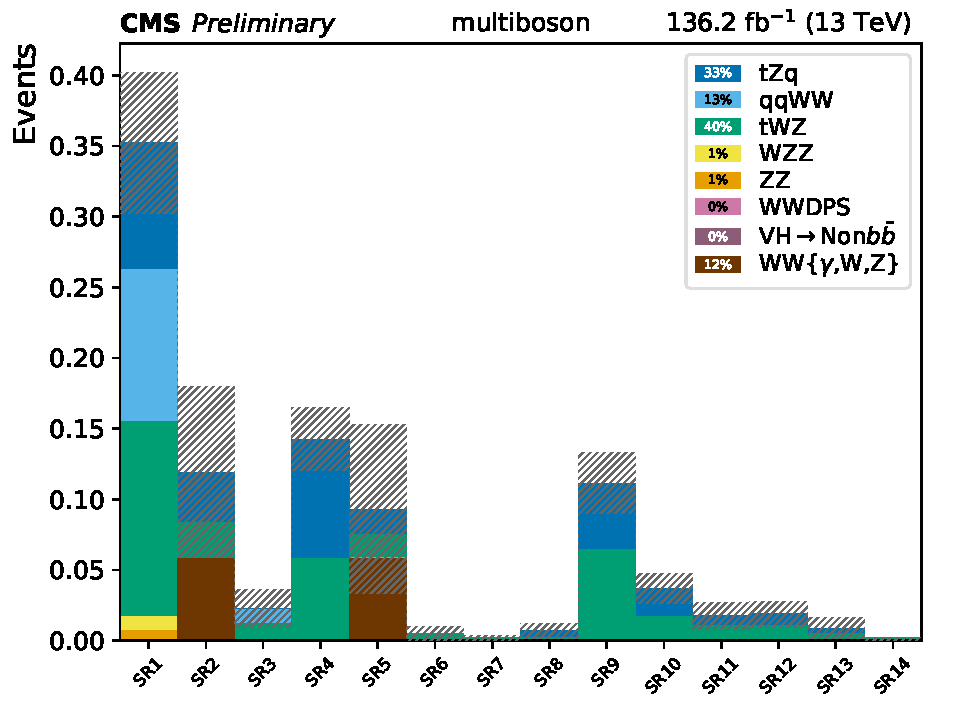
\includegraphics[width=.60\textwidth]{figs/ftan/h_multiboson.pdf}
    \caption{ Relative composition of multi-top (top) and multi-boson (bottom) rare backgrounds in the signal regions for all MC.}
    \label{fig:ftraressr}
\end{figure}

For the \smft analysis,
we apply uncertainties of 20\%, 11\%, and 11\% for Rare, \Xgamma, and \ttVV categories,
respectively, and 40\% for the \ttW and \ttZ categories. Also in the \smft analysis,
the \ttH category is assigned an uncertainty of 25\% to reflect the CMS \ttH 
measurement~\cite{CMS:Sirunyan2018hoz} which obtained a signal strength $\mu_{\ttH}$, defined
as the ratio between the measured $\ttH$ cross section and its SM expectation,
of $1.26^{+0.31}_{-0.26}$.

\FloatBarrier

\section{Nonprompt leptons}


Estimating the background from fake leptons requires care as simply
using fake leptons out of the box from simulation makes heavy assumptions on 
the accuracy of the simulation. It is better to somehow use data itself to estimate
the fake leptons from data.  We use the ``fake rate'', or ``tight-loose'', method
to estimate this background in a data-driven fashion via an extrapolation.

Recalling the two working points for lepton identification/isolation, loose and tight,
we use an orthogonal sideband (``application region'') of tight-loose-not-tight SS dilepton events 
(where one lepton is tight and the other is loose but not tight)
to estimate the fake contribution in the SRs (tight-tight SS dilepton events). 

The application region events can be weighted by a ``tight-to-loose'' ratio
(the probability for a loose non-prompt lepton to also pass the tight lepton selections)
to form the SR prediction. Defining $f$ as this probability, the fake contribution
in the SRs, $\mathrm{N}_\text{TT, fake}$  is given by
\begin{equation}
  N_\text{TT, fake} = \left(\frac{f}{1-f}\right) N_\text{TL}
  - \left(\frac{f}{1-f}\right)^2 N_\text{LL}
\end{equation}
where $N_\text{TL}$ represents the number of events in the application region
and $N_\text{LL}$ represents a similar, but smaller, application region where both
leptons pass the loose lepton selections but not the tight selections. The probability 
$f$ is parameterized by a modified lepton \pt (\ptcorr), lepton $\eta$, lepton flavor ($e$ or $\mu$),
data collection year, and trigger strategy (isolated, non-isolated). The minus sign
is needed for this ``double fake'' contribution to avoid overcounting (since
both tight-loose and loose-tight events are present in the application region and 
are extrapolated to the signal regions).

Now, unsurprisingly, $f \equiv f(\ptcorr,\eta)$ is measured in the ``measurement region''.
The measurement region is a sample of QCD multijet events, and thus, 
enriched in non-prompt leptons, with an event selection of
\begin{itemize}
\item specific auxiliary trigger, listed in Table~\ref{tab:frtrigs}
\item only one loose/denominator lepton (``fakeable object''/``FO'')
\item at least one jet with $\Delta R(\mathrm{jet},\mathrm{FO})>1$
\item $\ptmiss<20\GeV$
\item $\MT<20\GeV$
\end{itemize}
to make sure we select as much QCD in data in possible while minimizing
the amount of prompt leptons leaking into the measurement region.
Due to different trigger requirements and data collection periods, we derive
a total of 12 versions of the 2-dimensional \pt-$\eta$-binned fake rate
(electrons/muons, isolated triggers/non-isolated triggers, 2016/2017/2018)

We use a corrected lepton \pt, \ptcorr, to parameterize the fake rate
estimation in the fake rate estimation in order to reduce the dependency to
the mother parton \pt and the flavor composition of the
sample~\cite{CMS:AN14261}:

\begin{equation}
  \ptcorr = \left\{
        \begin{array}{ll}
            \pt \cdot (1+\max(0,I_\mathrm{mini}-I_1)) & \quad \text{if} \,\,\, \ptrel > I_3 \\[10pt]
            \max(\pt,\pt(\mathrm{jet}) \cdot I_2) & \quad \text{if} \,\,\, \ptrel \leq I_3
        \end{array}
      \right.
\end{equation}


While the requirements on \ptmiss and \MT suppress the
contribution from prompt leptons in the measurement region,
residual contributions from DY/\wjets/\ttjets (electroweak contamination)
need to be estimated and subtracted properly from the fake rate.
For this, we use simulation, but normalize in a high \MT/\ptmiss region.
Since the fake rate $f$ is the ratio of the number of tight leptons
to the number of loose leptons ($f=N_\mathrm{T}/N_\mathrm{L}$)
in the measurement region, we need to calculate $k$ for this region
($\MT>30\GeV$, $\ptmiss>30\GeV$) 
region and subtract from the numerator and denominator:
\begin{equation}
  f = \frac{N_\mathrm{T} - k \cdot N_\mathrm{T}^\text{EWK}}{N_\mathrm{L} - k \cdot N_\mathrm{L}^\text{EWK}}
\end{equation}
where $N^\text{EWK}$ represents the electroweak contamination.
These correction factors, $k$, are obtained by fitting the sum of two templates
derived from MC, one for QCD and one for the sum of electroweak processes
(DY, \wjets, \ttjets). The normalization of the elctroweak processes is extracted
from the fit and yields $k$. Since the shape of the non-prompt component
might not be well-modeled, we performa cross-check by repeating the fit and replacing the QCD
MC template with a data-drive template from events failing the isolation requirements.
The nominal and alternative fits for electrons and muons are shown in 
Fig.~\ref{fig:EWKnormalization2017iso} for 2017 data with isolated triggers, for example.
The resulting normalization corrections for the the full set of years and both trigger types
are shown in Table~\ref{tab:ewkfits}.

Two-dimensional fake rate maps for isolated triggers for 2017 data and QCD simulation
are shown in Fig.~\ref{fig:QCDFRMuEleRaw2017iso}.
One can see that prior to the electroweak subtraction, the fake rates increase drastically
at high lepton \pt. This is expected, as the probability for true/prompt leptons
from electroweak proceesses to pass the tight selection is large (Otherwise our lepton
selections would not be doing their job in the first place.)
To better visualize the fake rates, 
one-dimensional projections onto the \ptcorr axis for each of the three years
are shown in Figs.~\ref{fig:QCDFRMuEle2016isoandnoniso}, \ref{fig:QCDFRMuEle2017isoandnoniso},
and \ref{fig:QCDFRMuEle2018isoandnoniso}. One sees good agreement between
the data-driven fake rate and fake rate calculated directly with QCD MC, though
this is not at all expected or needed. Also note the large uncertainties at high \ptcorr,
which is due to the uncertainty associated with the electroweak subtraction procedure.


\begin{figure}[!hbtp]
  \centering
  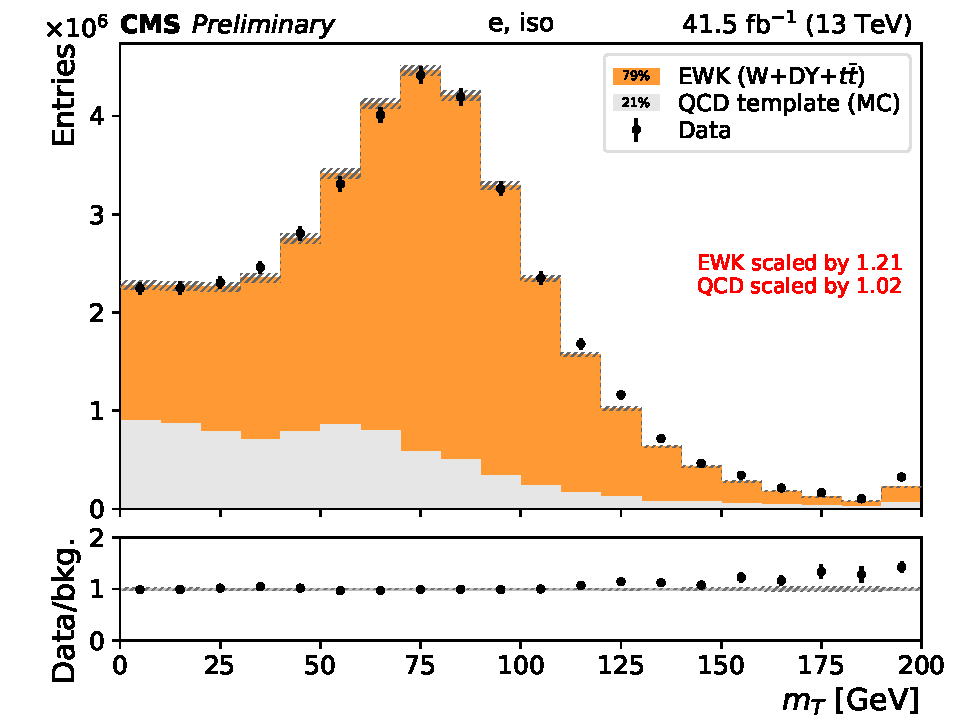
\includegraphics[width=.45\textwidth]{figs/ssan/fakerate/derivation/y2017/y2017_el_iso_mt_lin_postfit_mctemp.pdf}
  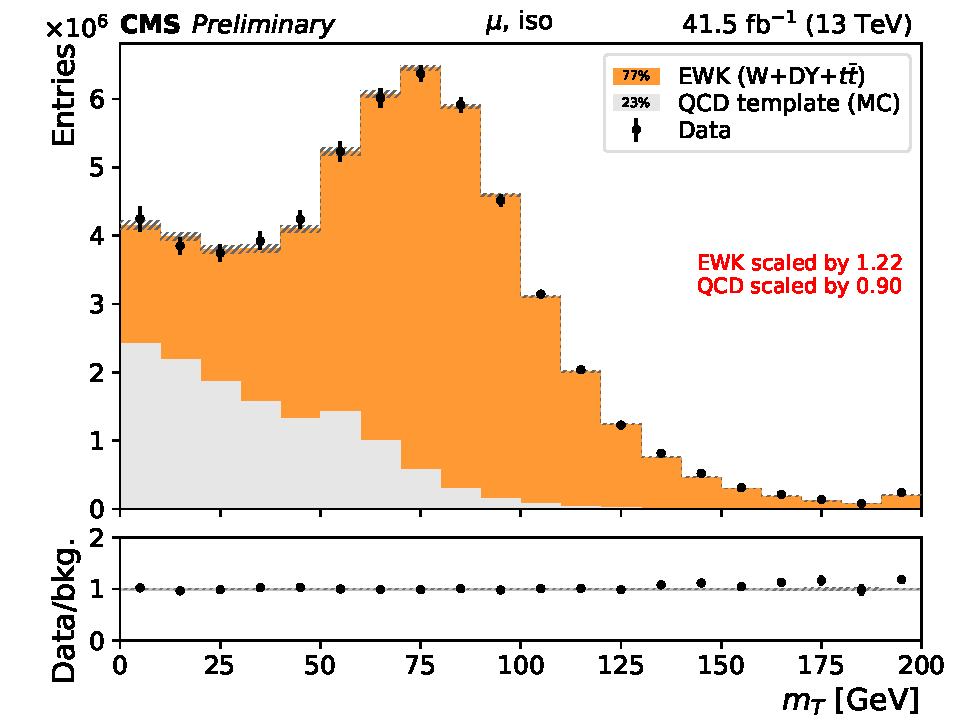
\includegraphics[width=.45\textwidth]{figs/ssan/fakerate/derivation/y2017/y2017_mu_iso_mt_lin_postfit_mctemp.pdf} \\
  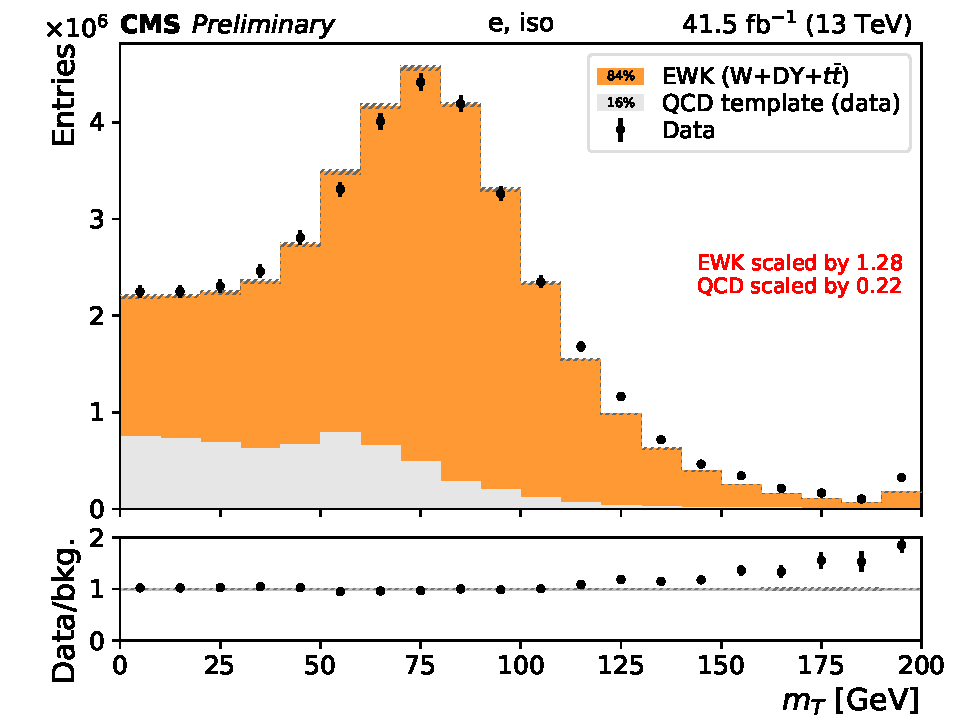
\includegraphics[width=.45\textwidth]{figs/ssan/fakerate/derivation/y2017/y2017_el_iso_mt_lin_postfit_datatemp.pdf}
  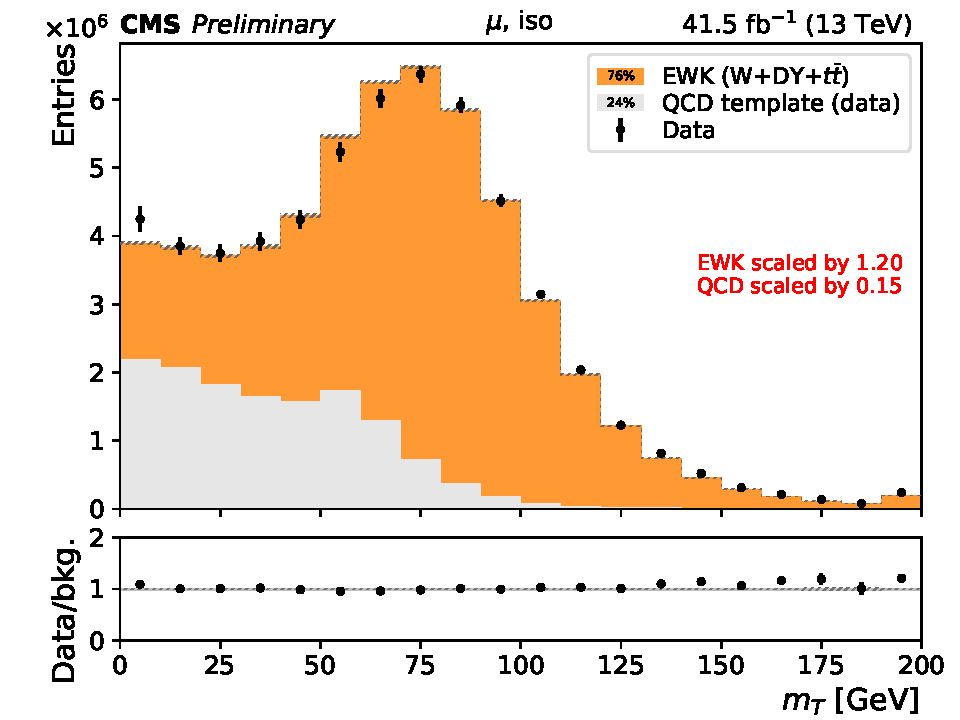
\includegraphics[width=.45\textwidth]{figs/ssan/fakerate/derivation/y2017/y2017_mu_iso_mt_lin_postfit_datatemp.pdf}
  \caption{ 
  Fitted $M_T$ distribution used to derive the
  normalization of electroweak samples (DY, \wjets, \ttjets) in the fake rate measurement region.
  Electrons are shown on the left, muons on the right.
  From top to bottom, the results from the nominal selection ($\ptmiss>30~\GeV$ and 
  lepton $\pt > 20~\GeV$) with the QCD MC template and alternative data QCD template are shown. 
  Data and MC conditions correspond to isolated triggers in 2017.
  }
  \label{fig:EWKnormalization2017iso}
  \end{figure}

\begin{table}[htbp]
  \begin{center}
      \small
    {\renewcommand{\arraystretch}{1.3}
      \begin{tabular}{ll|cc|cc}
          \hline
          & & \multicolumn{2}{c|}{isolated triggers} & \multicolumn{2}{c}{non-isolated triggers} \\ %\cline{3-6}
                    & & $e$ &  $\mu$ & $e$ & $\mu$ \\ \hline
          \multirow{2}{*}{2016} & MC template        & 1.240 & 1.189 & 1.258 & 1.164 \\
                & data template      & 1.294 & 1.154 & 1.337 & 1.131 \\ \hline
          \multirow{2}{*}{2017} & MC  template       & 1.215 & 1.222 & 1.208 & 1.202 \\
                & data template      & 1.277 & 1.195 & 1.298 & 1.178 \\ \hline
          \multirow{2}{*}{2018} & MC  template       & 1.216 & 1.277 & 1.195 & 1.286 \\
                & data template      & 1.285 & 1.247 & 1.300 & 1.249 \\ \hline
      \end{tabular}}
      \caption{Normalization scale factors for electroweak samples derived with two different $M_T$ templates for QCD: MC and data (the data template refers to the inverted isolation region).}
      \label{tab:ewkfits}
  \end{center}
\end{table}

\FloatBarrier

  \begin{figure}[!hbtp]
    \centering
    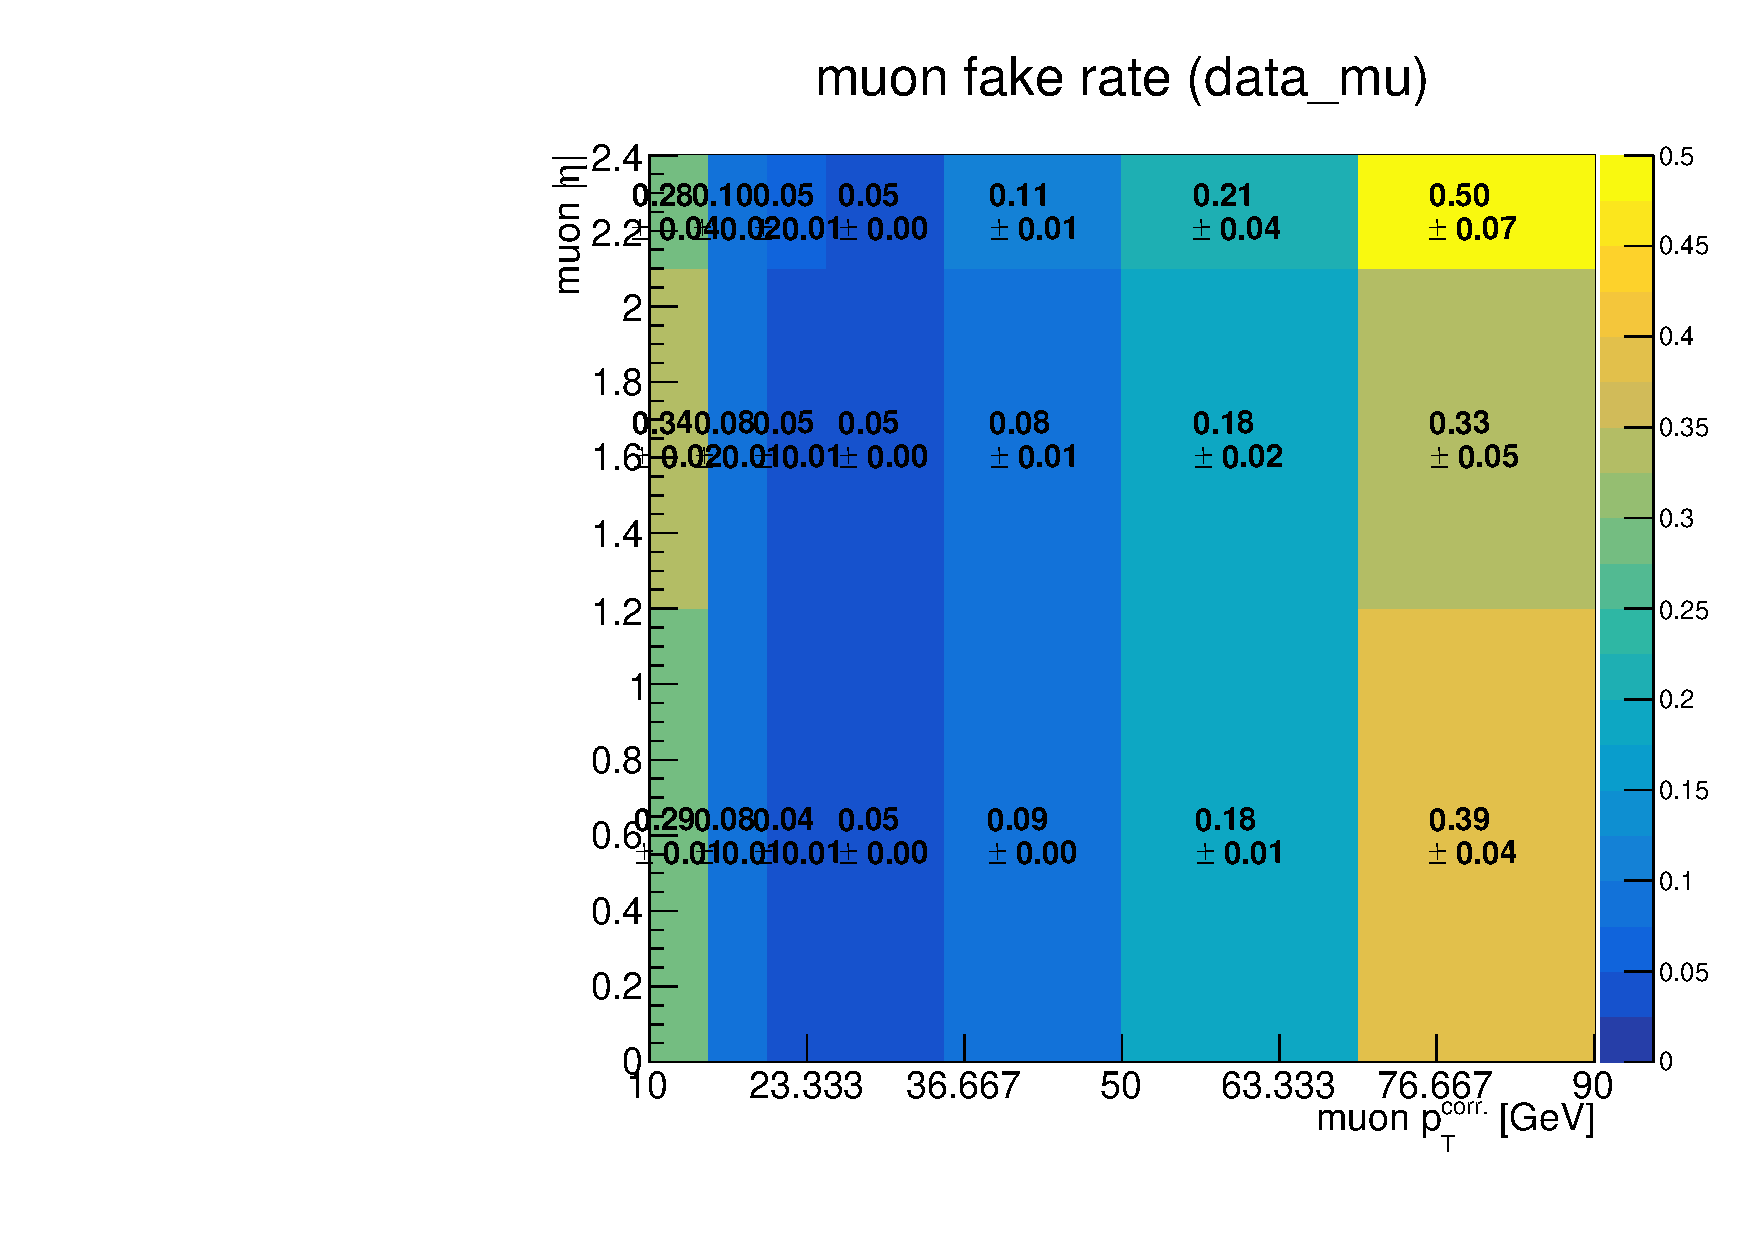
\includegraphics[width=.42\textwidth]{figs/ssan/fakerate/derivation/y2017/y2017_mu_fr_cone_data_mu_LooseEMVA_IsoTrigs.pdf}
    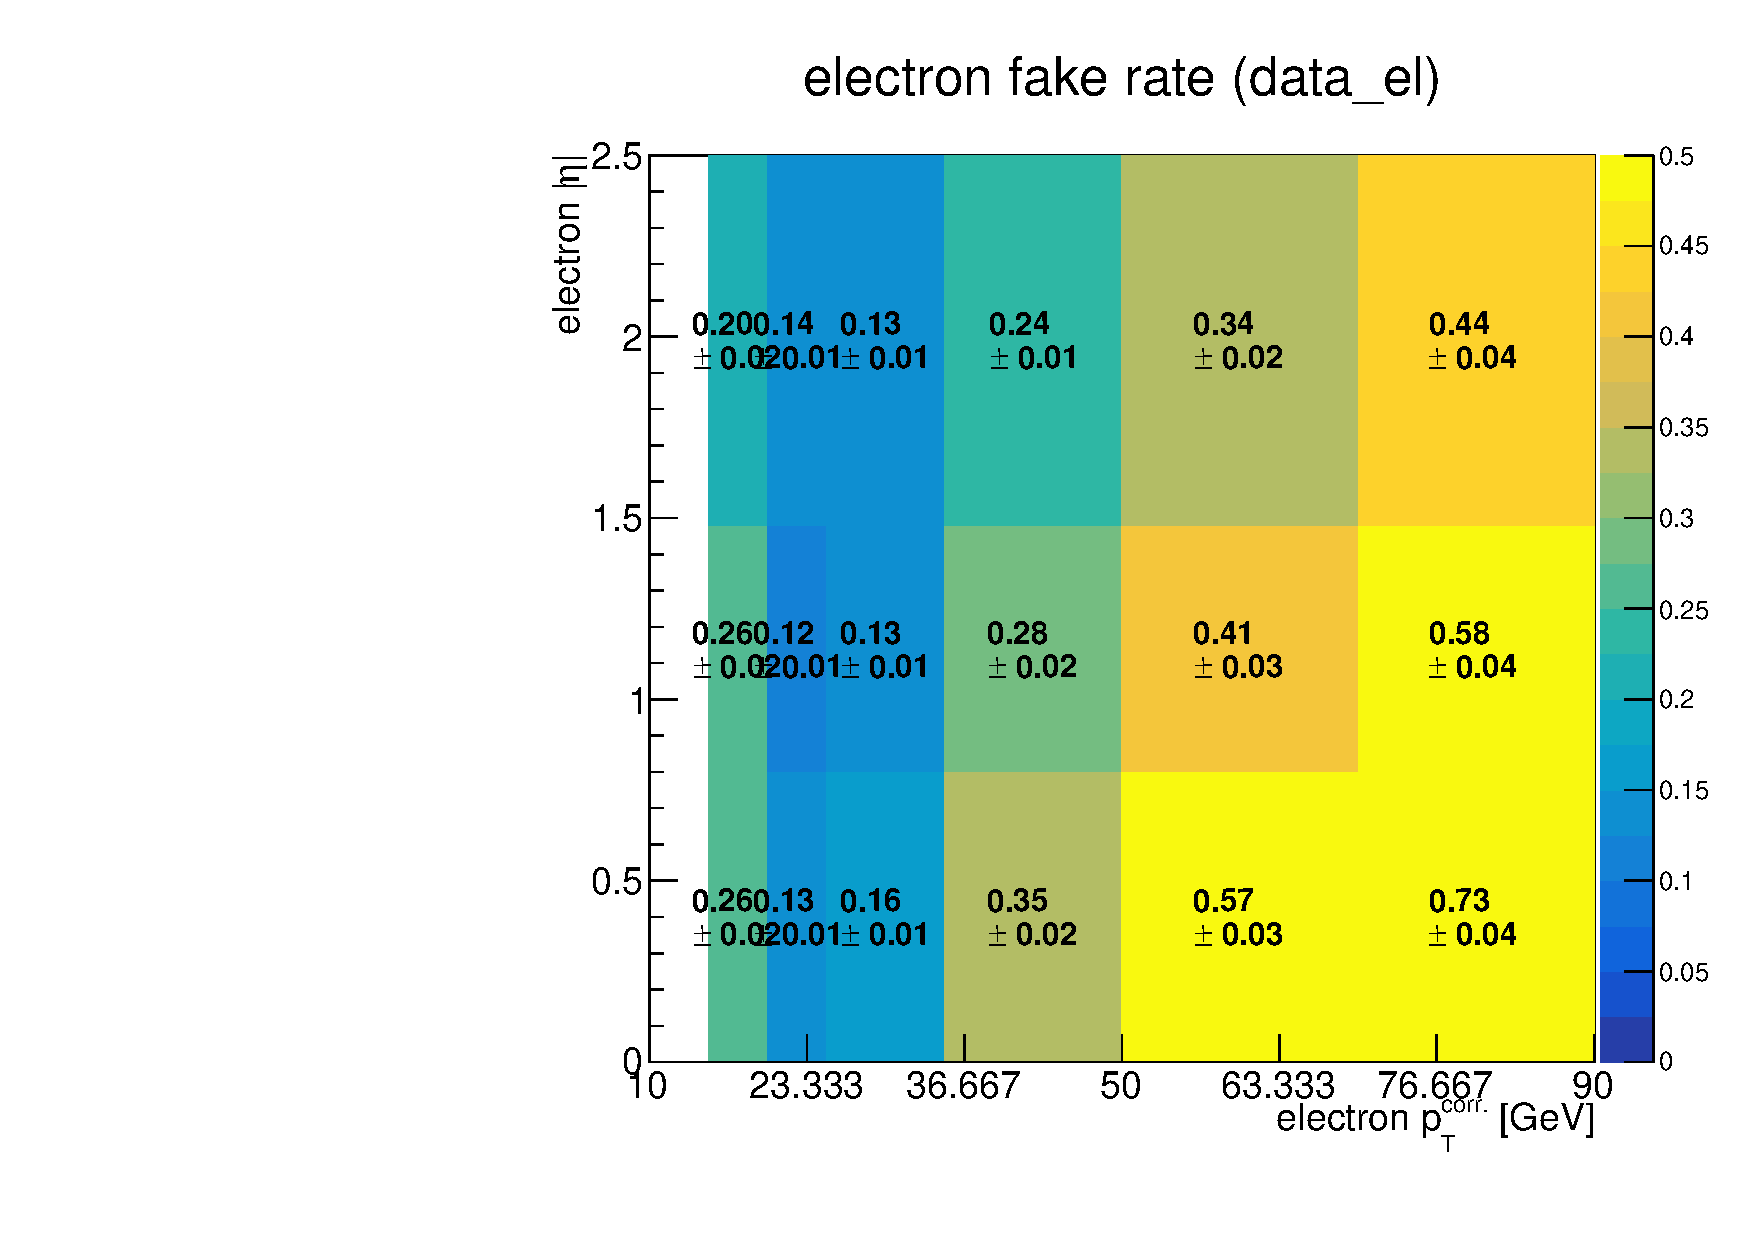
\includegraphics[width=.42\textwidth]{figs/ssan/fakerate/derivation/y2017/y2017_el_fr_cone_data_el_LooseEMVA_IsoTrigs.pdf}
    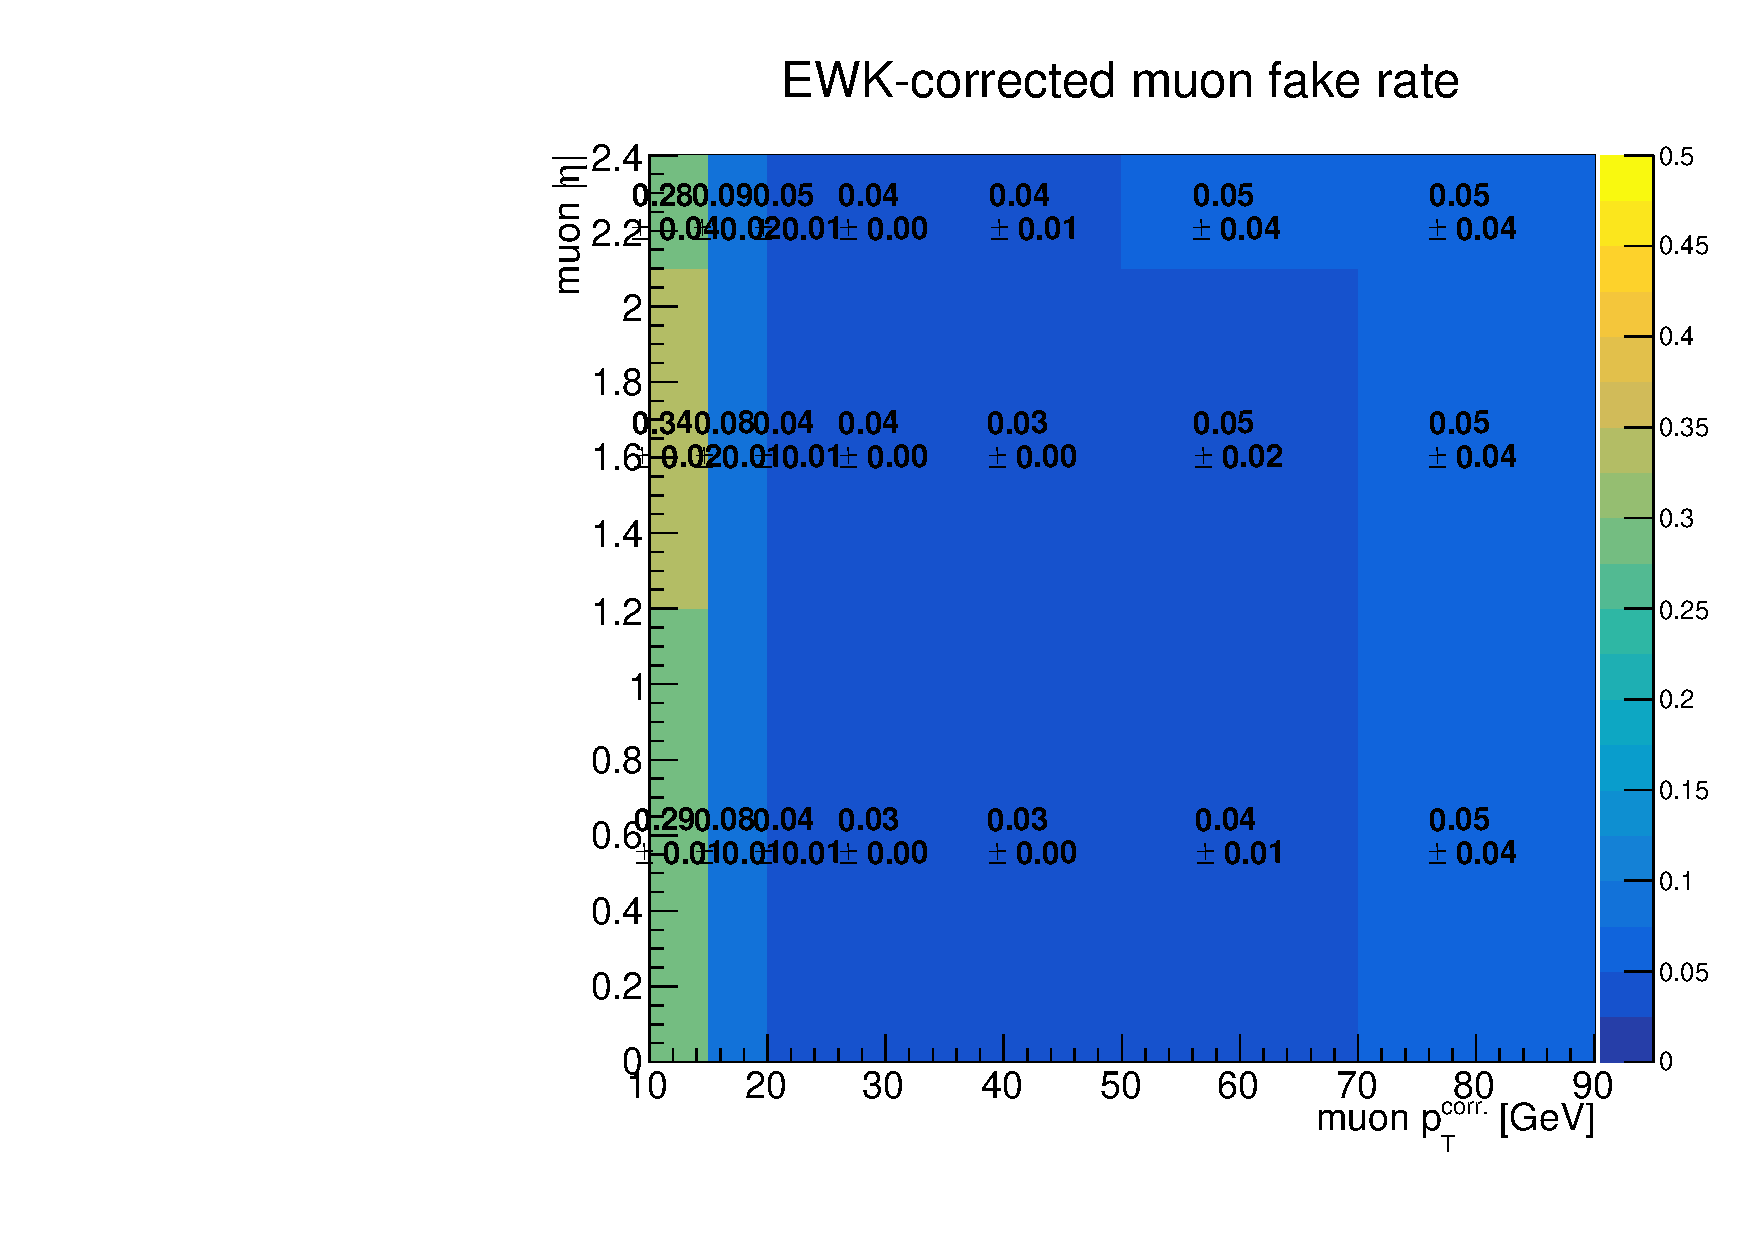
\includegraphics[width=.42\textwidth]{figs/ssan/fakerate/derivation/y2017/y2017_ewkCorFR_muon_IsoTrigs.pdf}
    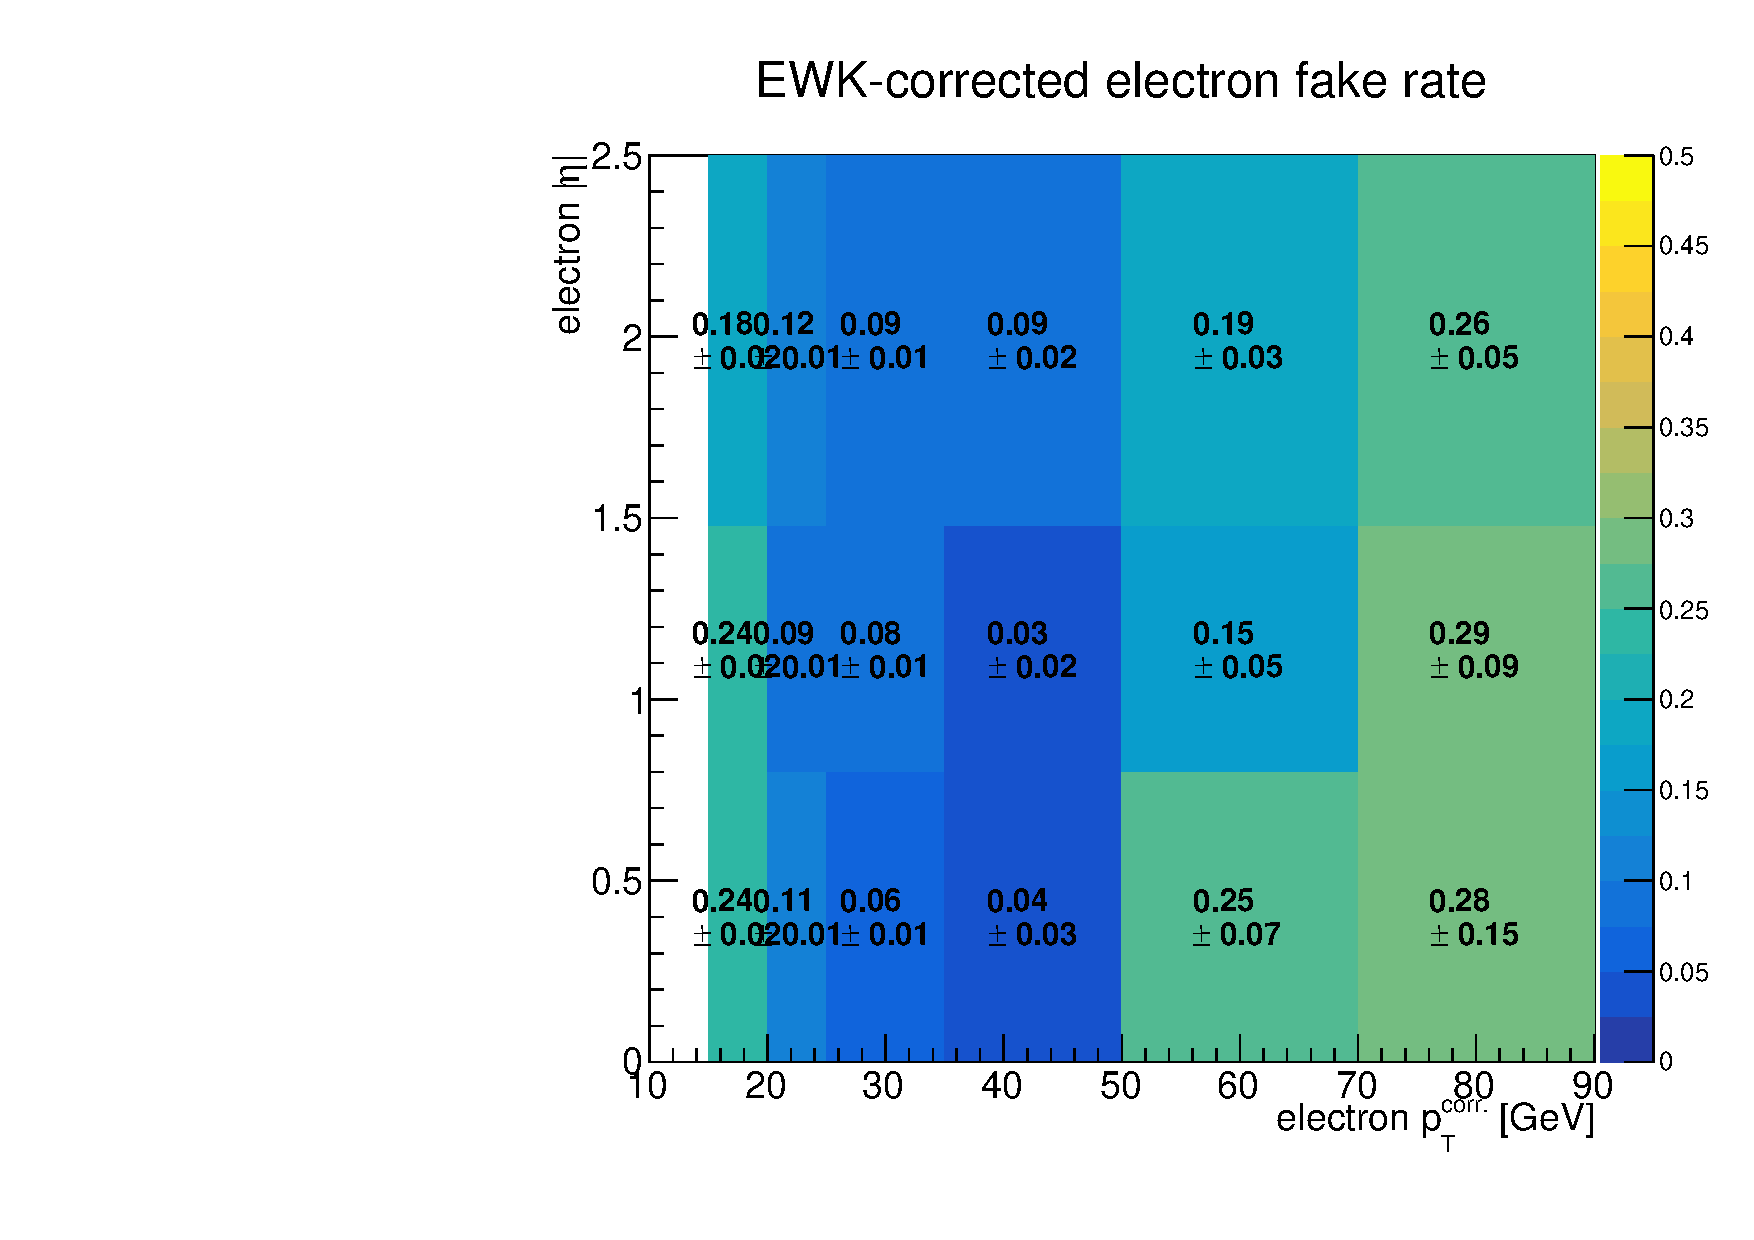
\includegraphics[width=.42\textwidth]{figs/ssan/fakerate/derivation/y2017/y2017_ewkCorFR_electron_IsoTrigs.pdf}
    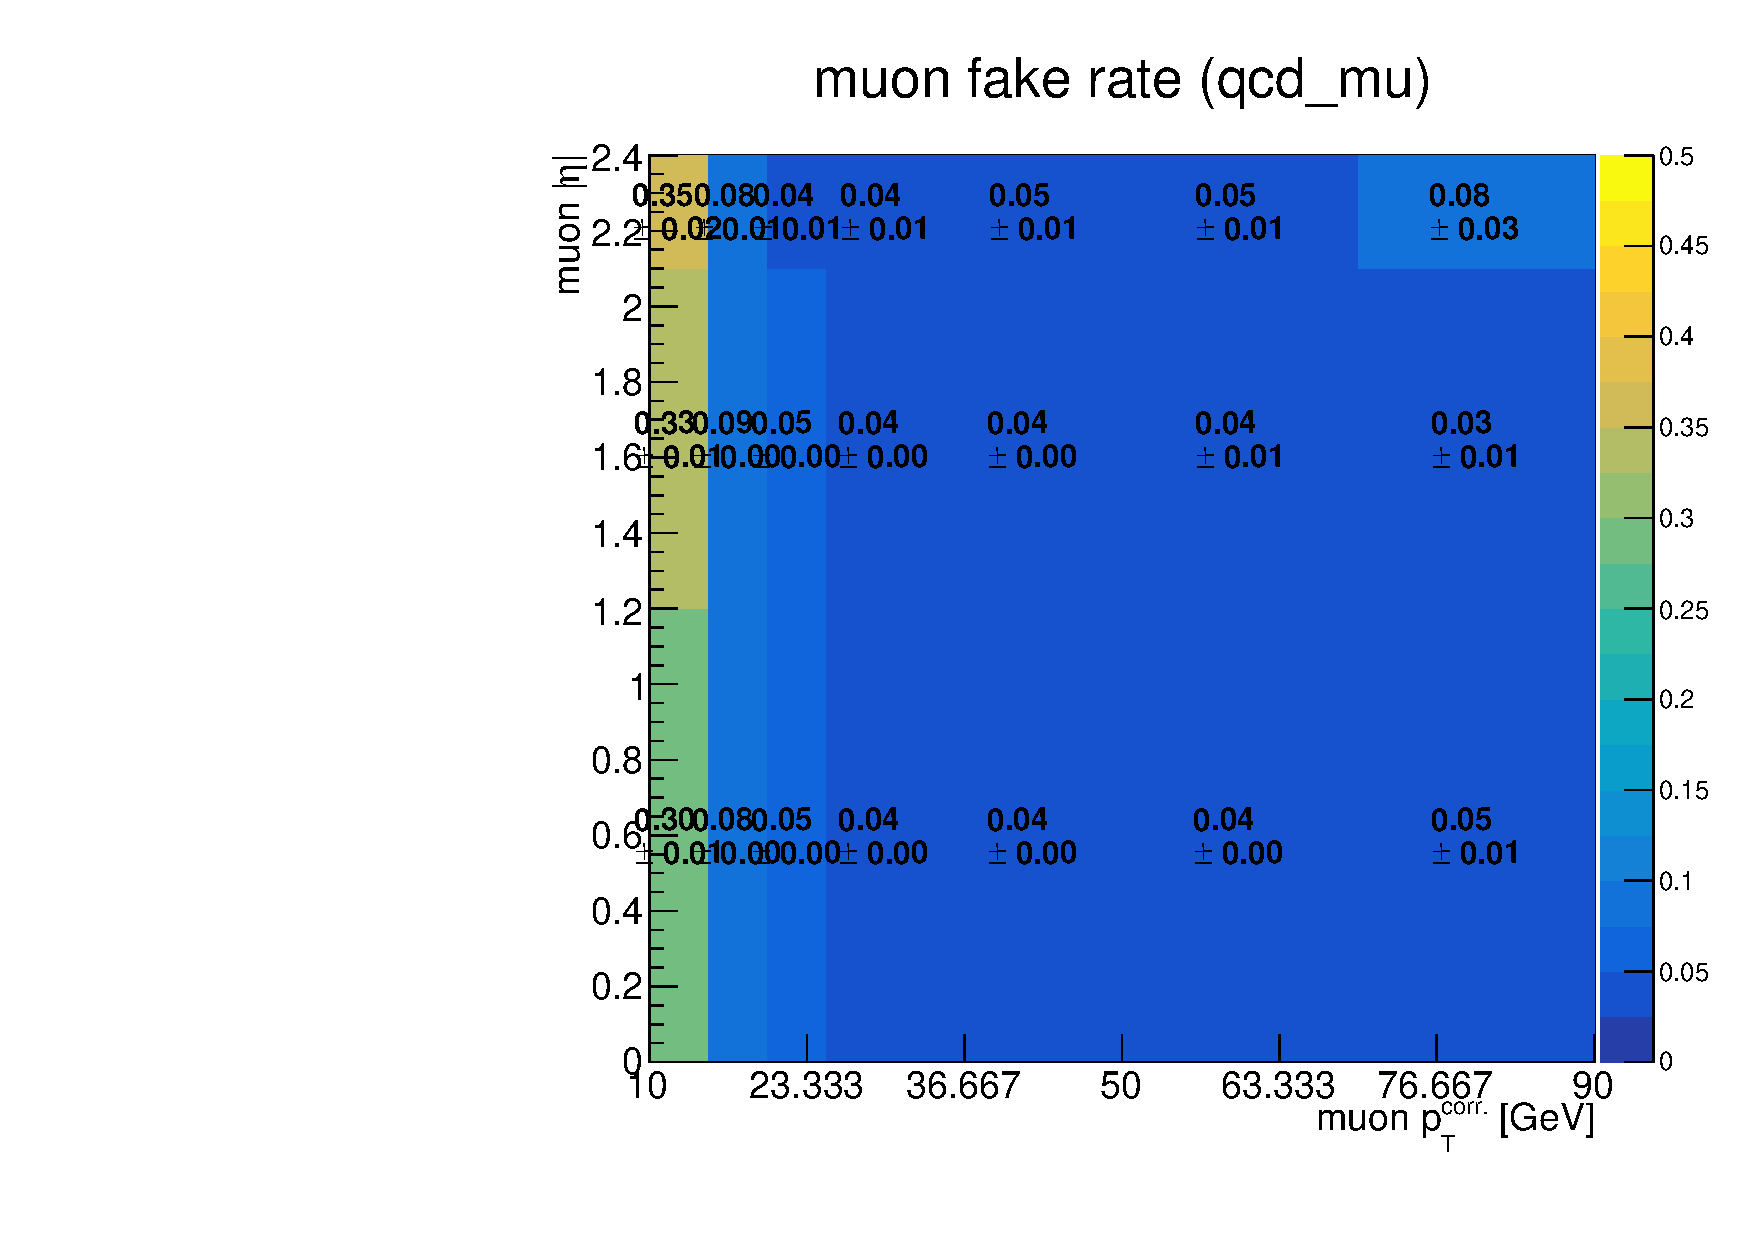
\includegraphics[width=.42\textwidth]{figs/ssan/fakerate/derivation/y2017/y2017_mu_fr_cone_qcd_mu_LooseEMVA_IsoTrigs.pdf}
    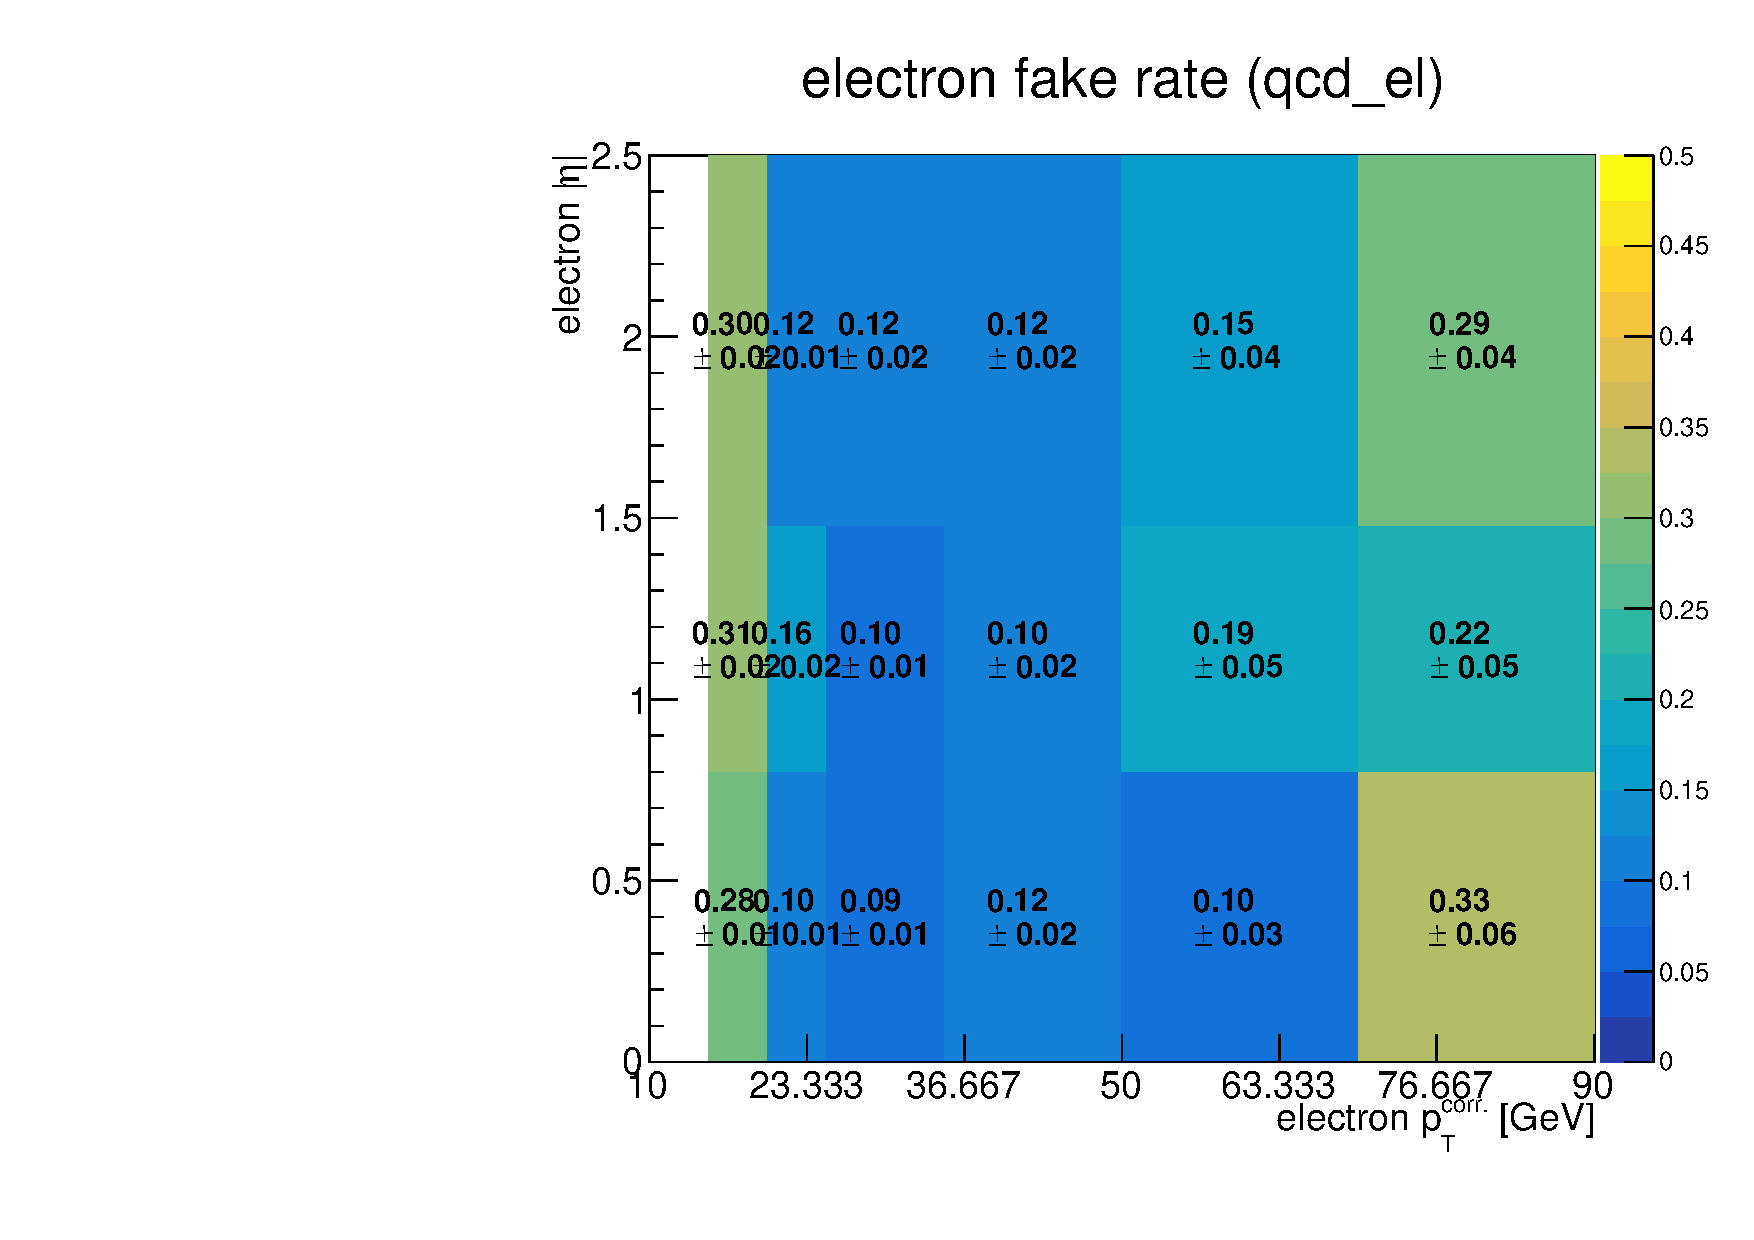
\includegraphics[width=.42\textwidth]{figs/ssan/fakerate/derivation/y2017/y2017_el_fr_cone_qcd_el_LooseEMVA_IsoTrigs.pdf}
        \caption{  Two-dimensional fake rate maps for isolated triggers for muons (left) and electrons (right),
        for 2017 data uncorrected (top),
        2017 data corrected for electroweak contamination (middle) and 2017 QCD simulation (bottom).
        }
    \label{fig:QCDFRMuEleRaw2017iso}
    \end{figure}

    %%%%%%%%%%%%%%%%%%%%%%%%%%%%%%%%%%%%
\begin{figure}[!hbtp]
  \centering
  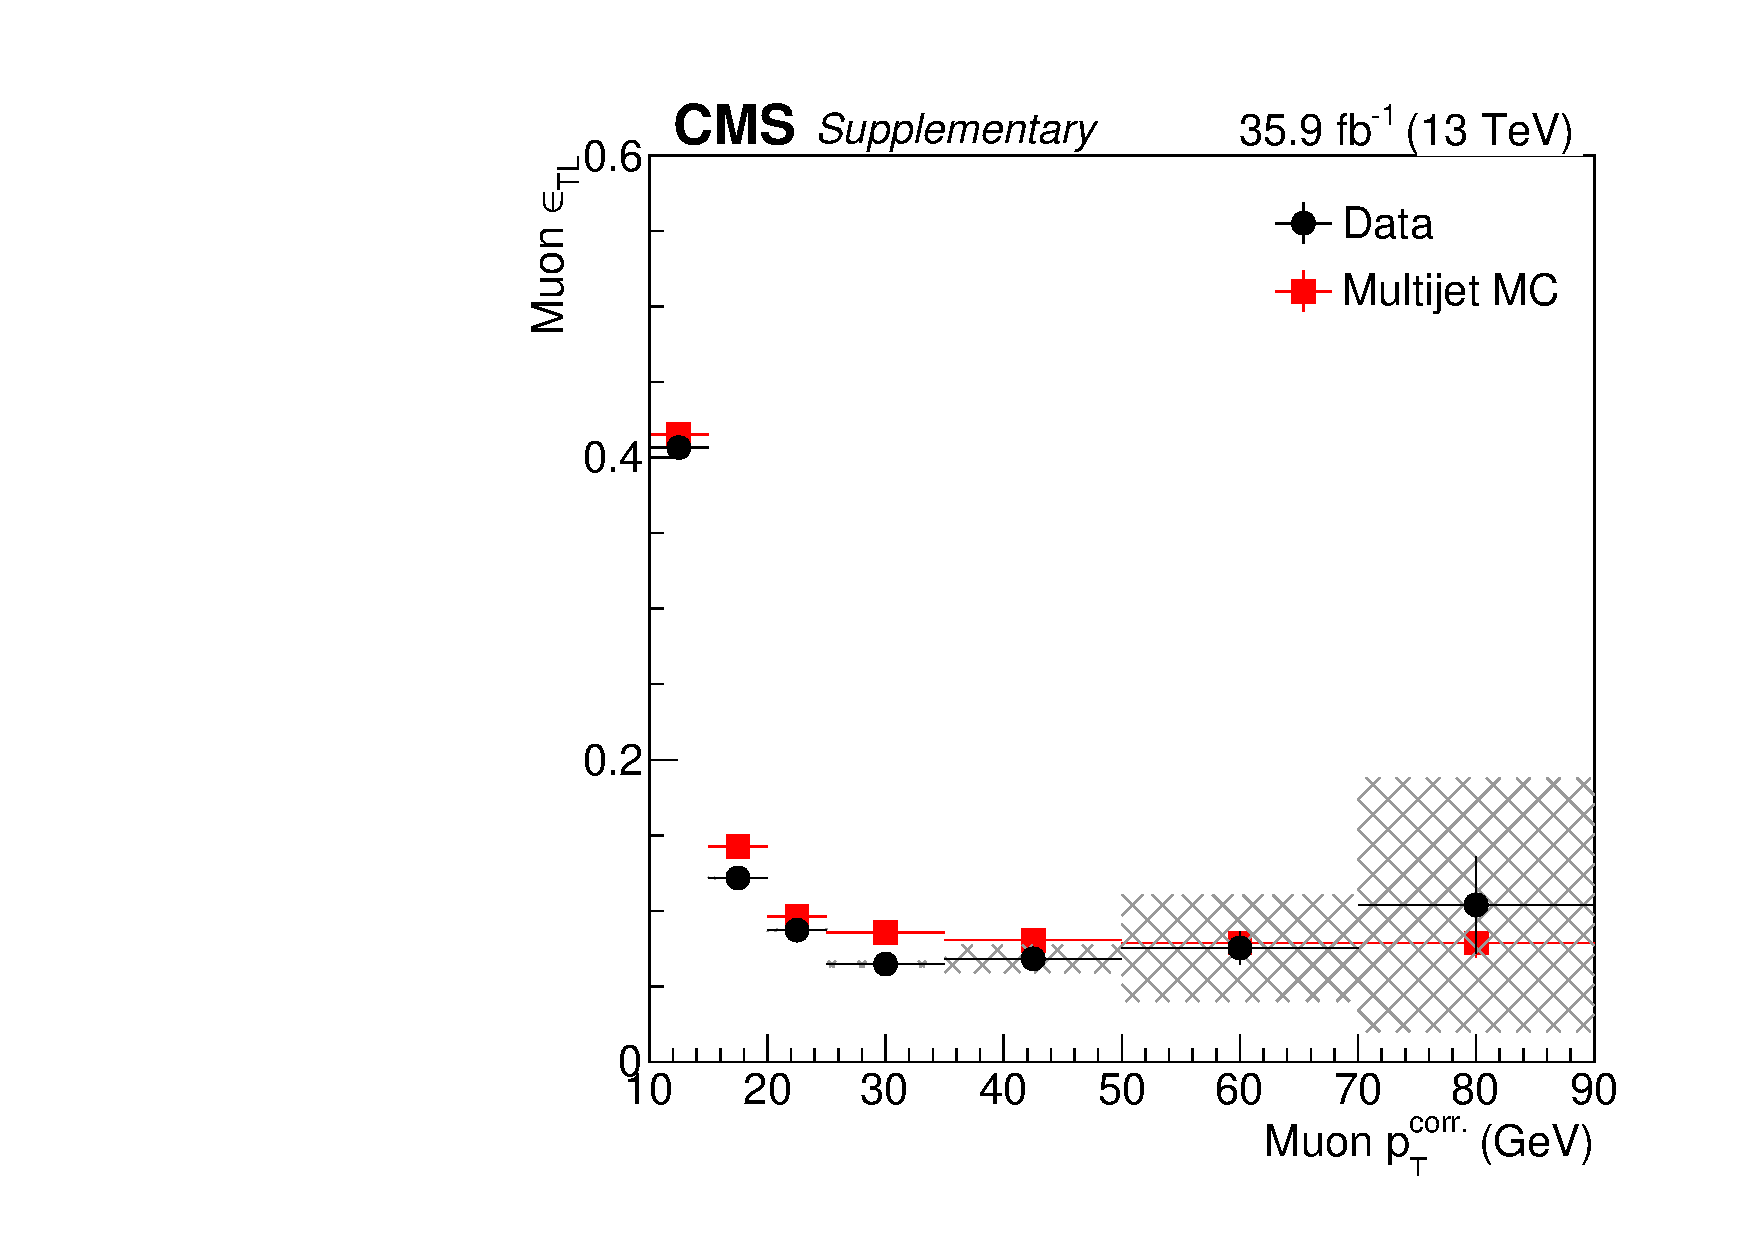
\includegraphics[width=.45\textwidth]{figs/ssan/fakerate/derivation/y2016/y2016_mu_1dfr_cone_LooseEMVA_IsoTrigs.pdf}
  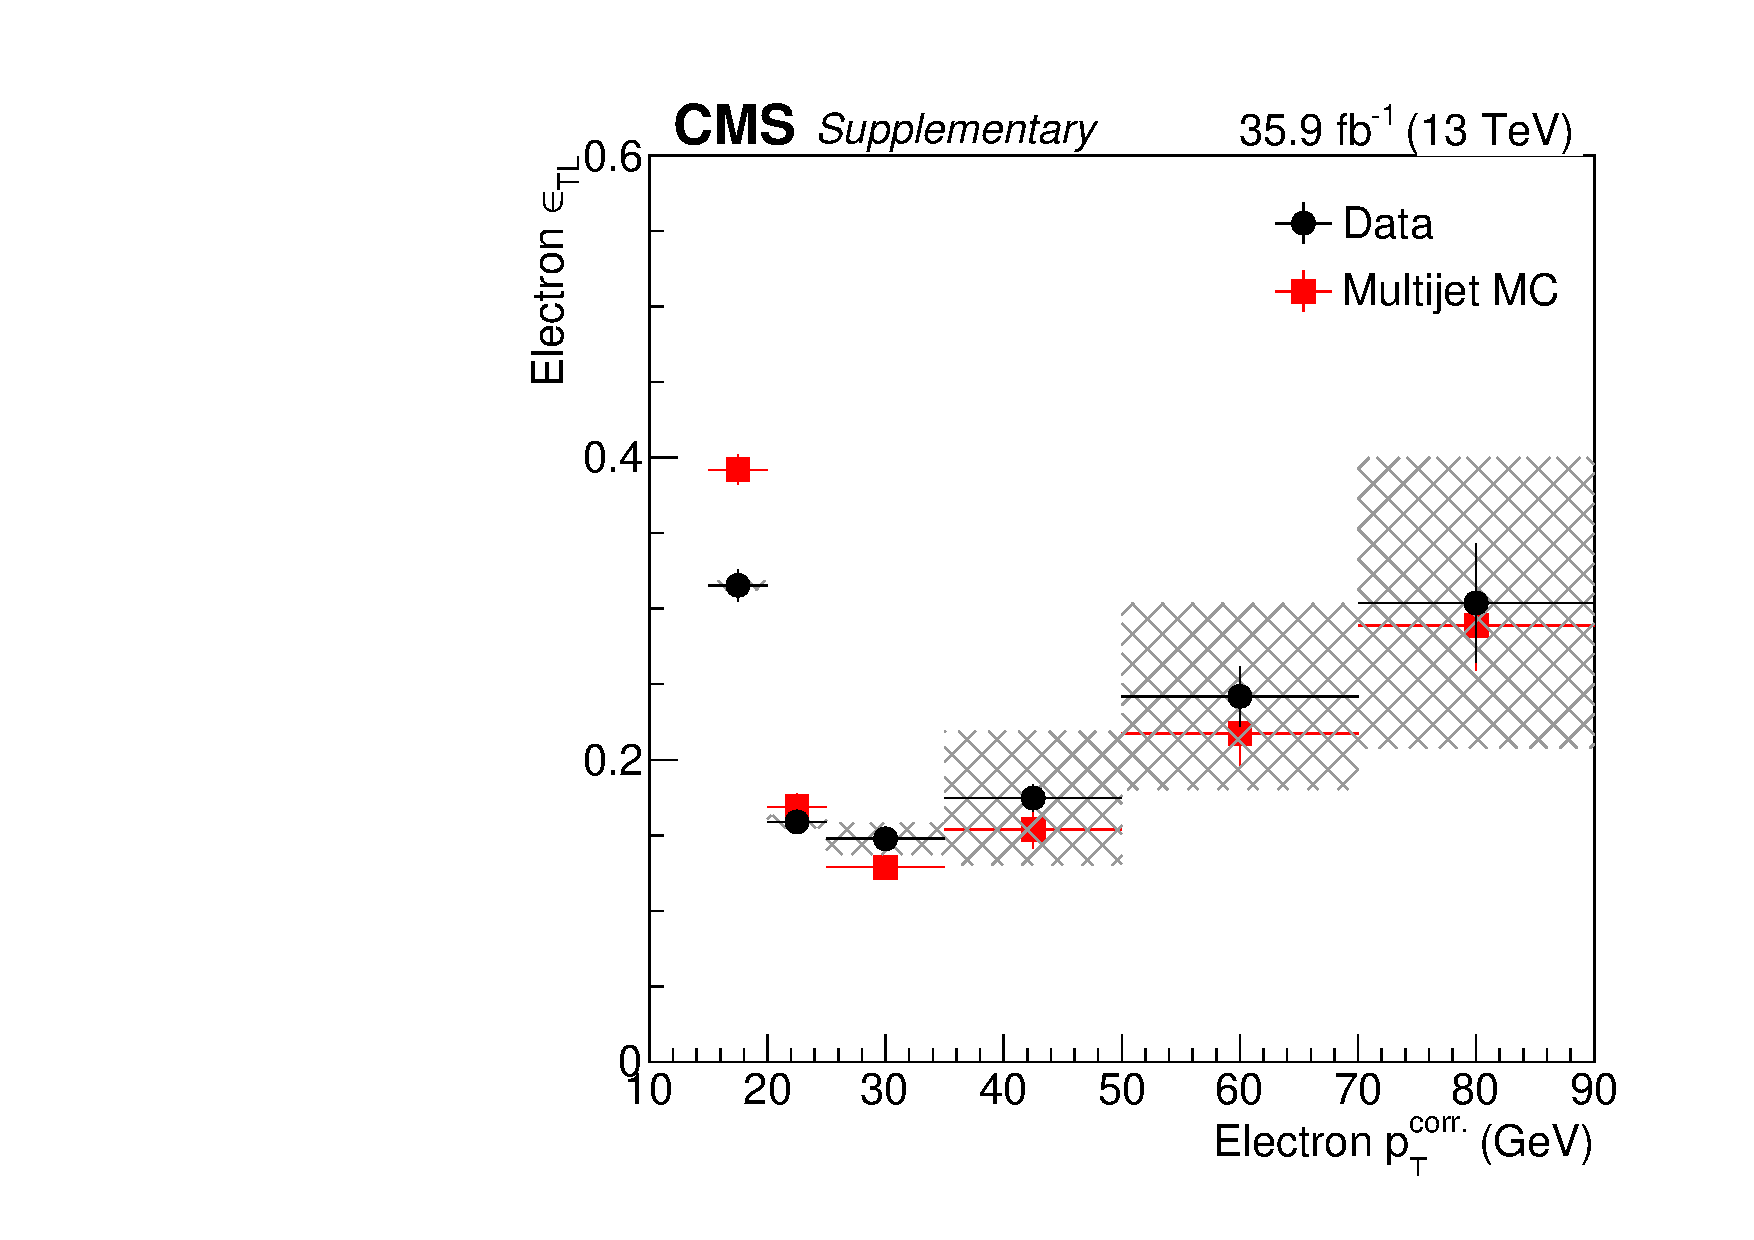
\includegraphics[width=.45\textwidth]{figs/ssan/fakerate/derivation/y2016/y2016_el_1dfr_cone_LooseEMVA_IsoTrigs.pdf} \\
  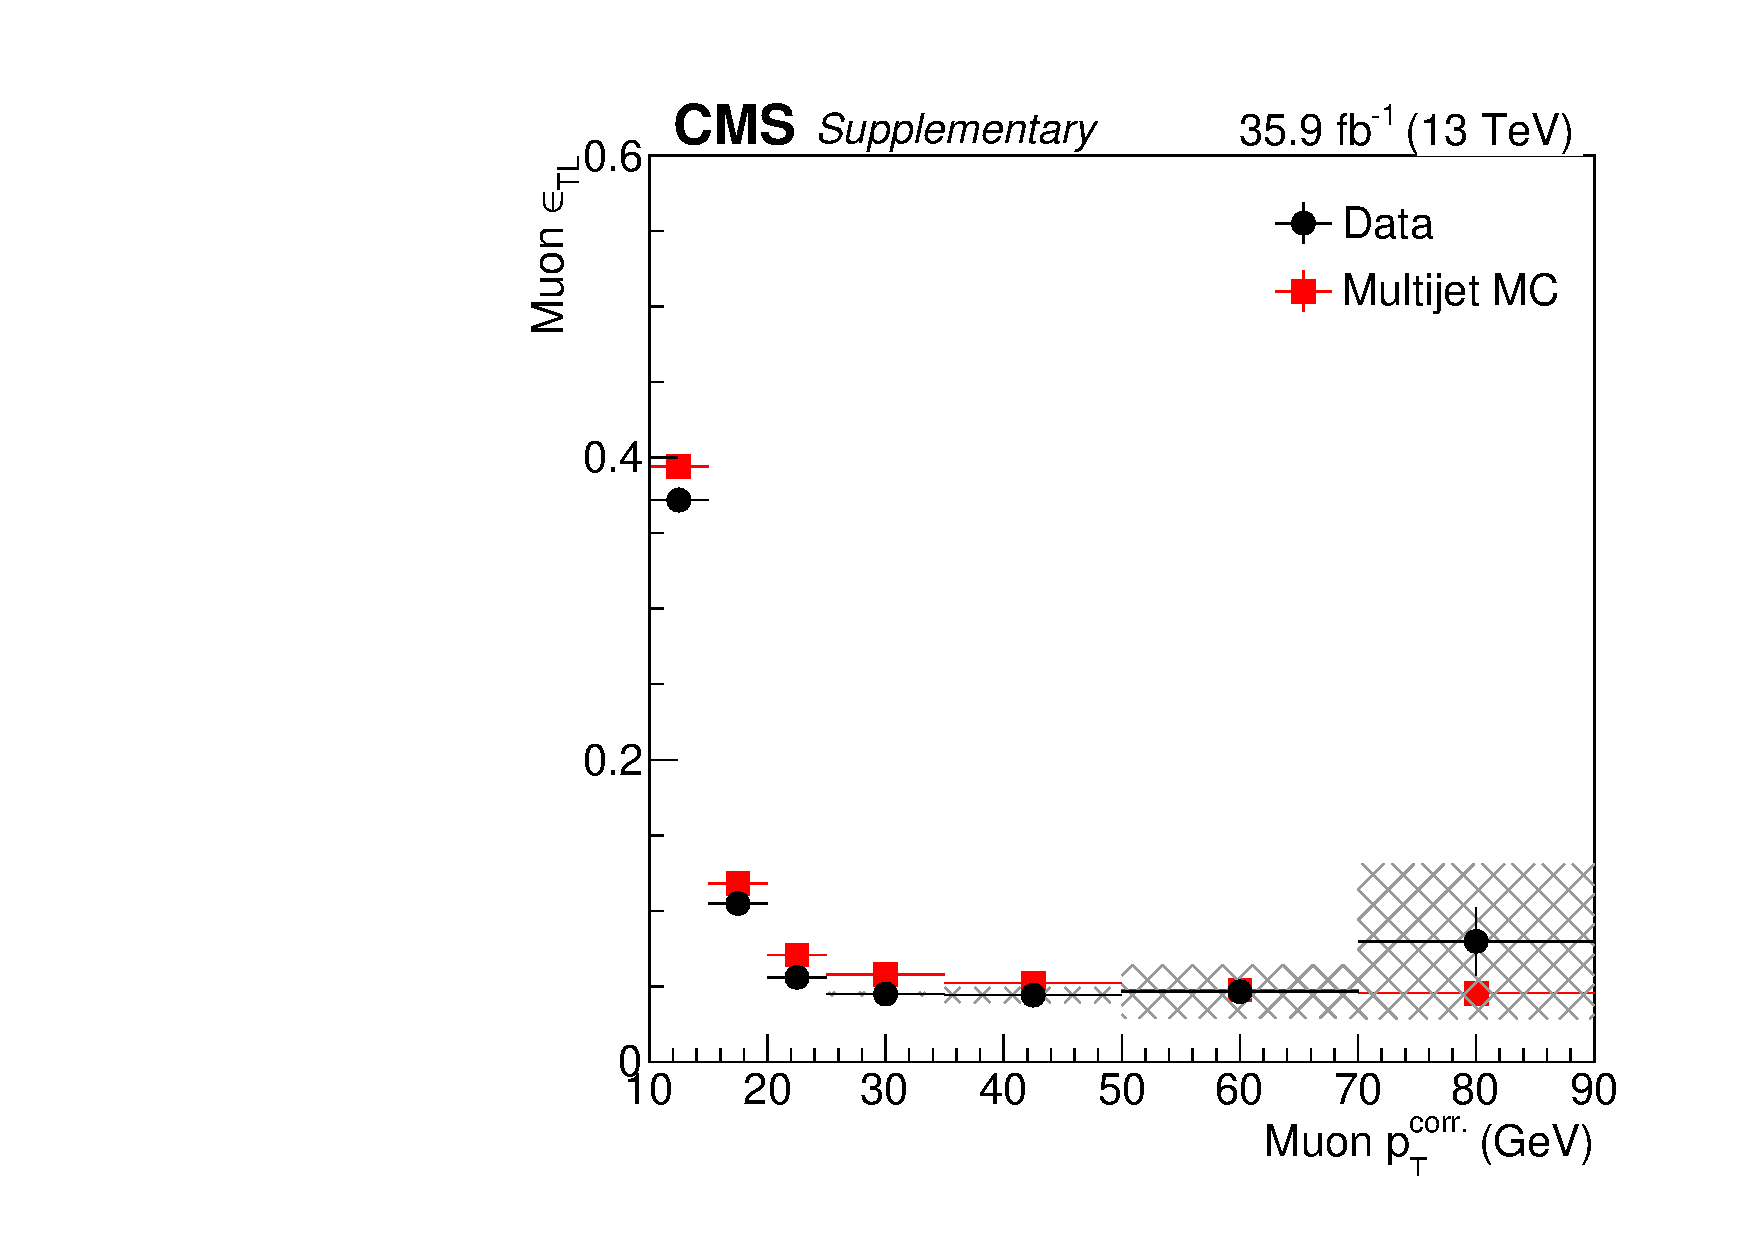
\includegraphics[width=.45\textwidth]{figs/ssan/fakerate/derivation/y2016/y2016_mu_1dfr_cone_LooseEMVA.pdf}
  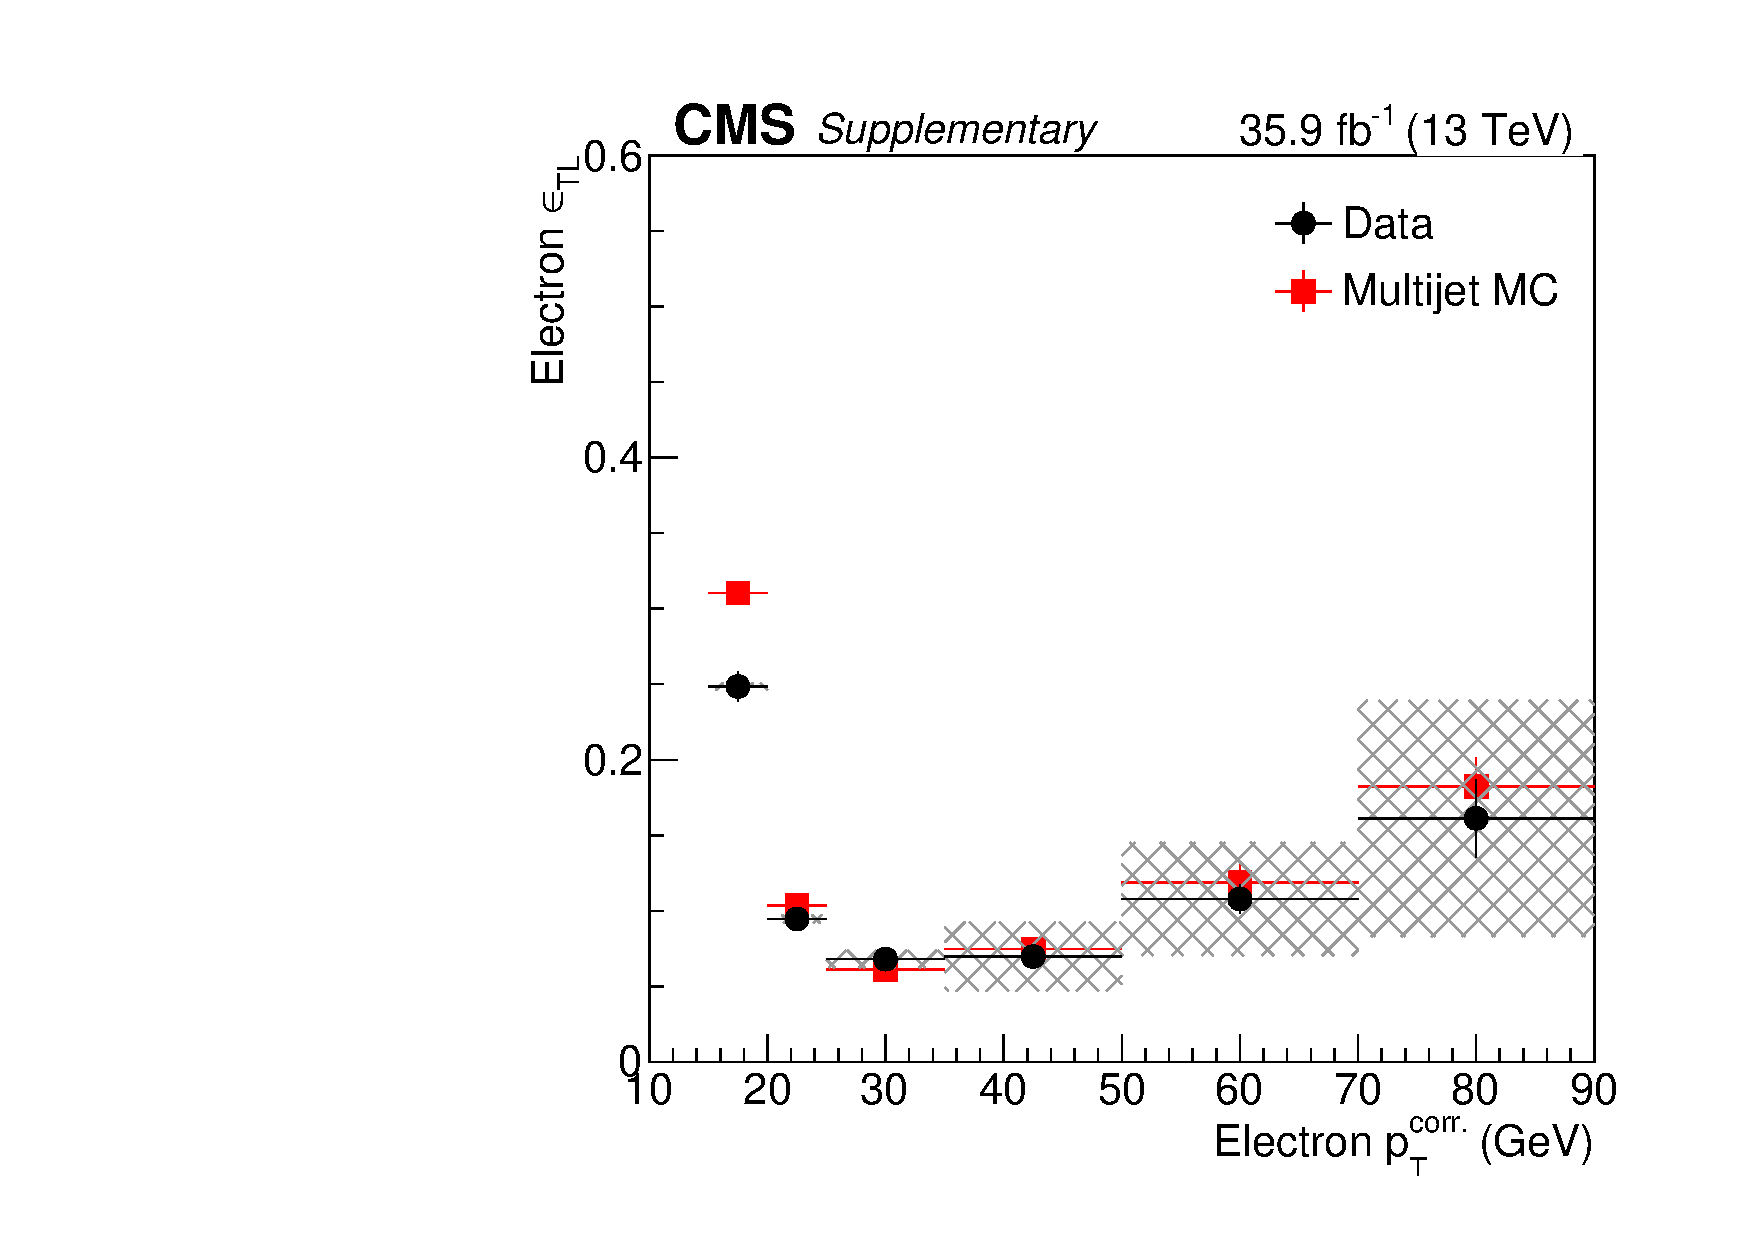
\includegraphics[width=.45\textwidth]{figs/ssan/fakerate/derivation/y2016/y2016_el_1dfr_cone_LooseEMVA.pdf}
  \caption{Electroweak contamination-corrected data fake rate projected vs \pt for 2016 data (black) and 2016 QCD simulation (red),
   for muons (left) and electrons (right). Isolated triggers are on top and non-isolated triggers on bottom.
      The shaded band in the projection is the systematic uncertainty related to the electroweak contamination.}
  \label{fig:QCDFRMuEle2016isoandnoniso}
  \end{figure}
  %%%%%%%%%%%%%%%%%%%%%%%%%%%%%%%%%%%%%%
  %%%%%%%%%%%%%%%%%%%%%%%%%%%%%%%%%%%%
  \begin{figure}[!hbtp]
  \centering
  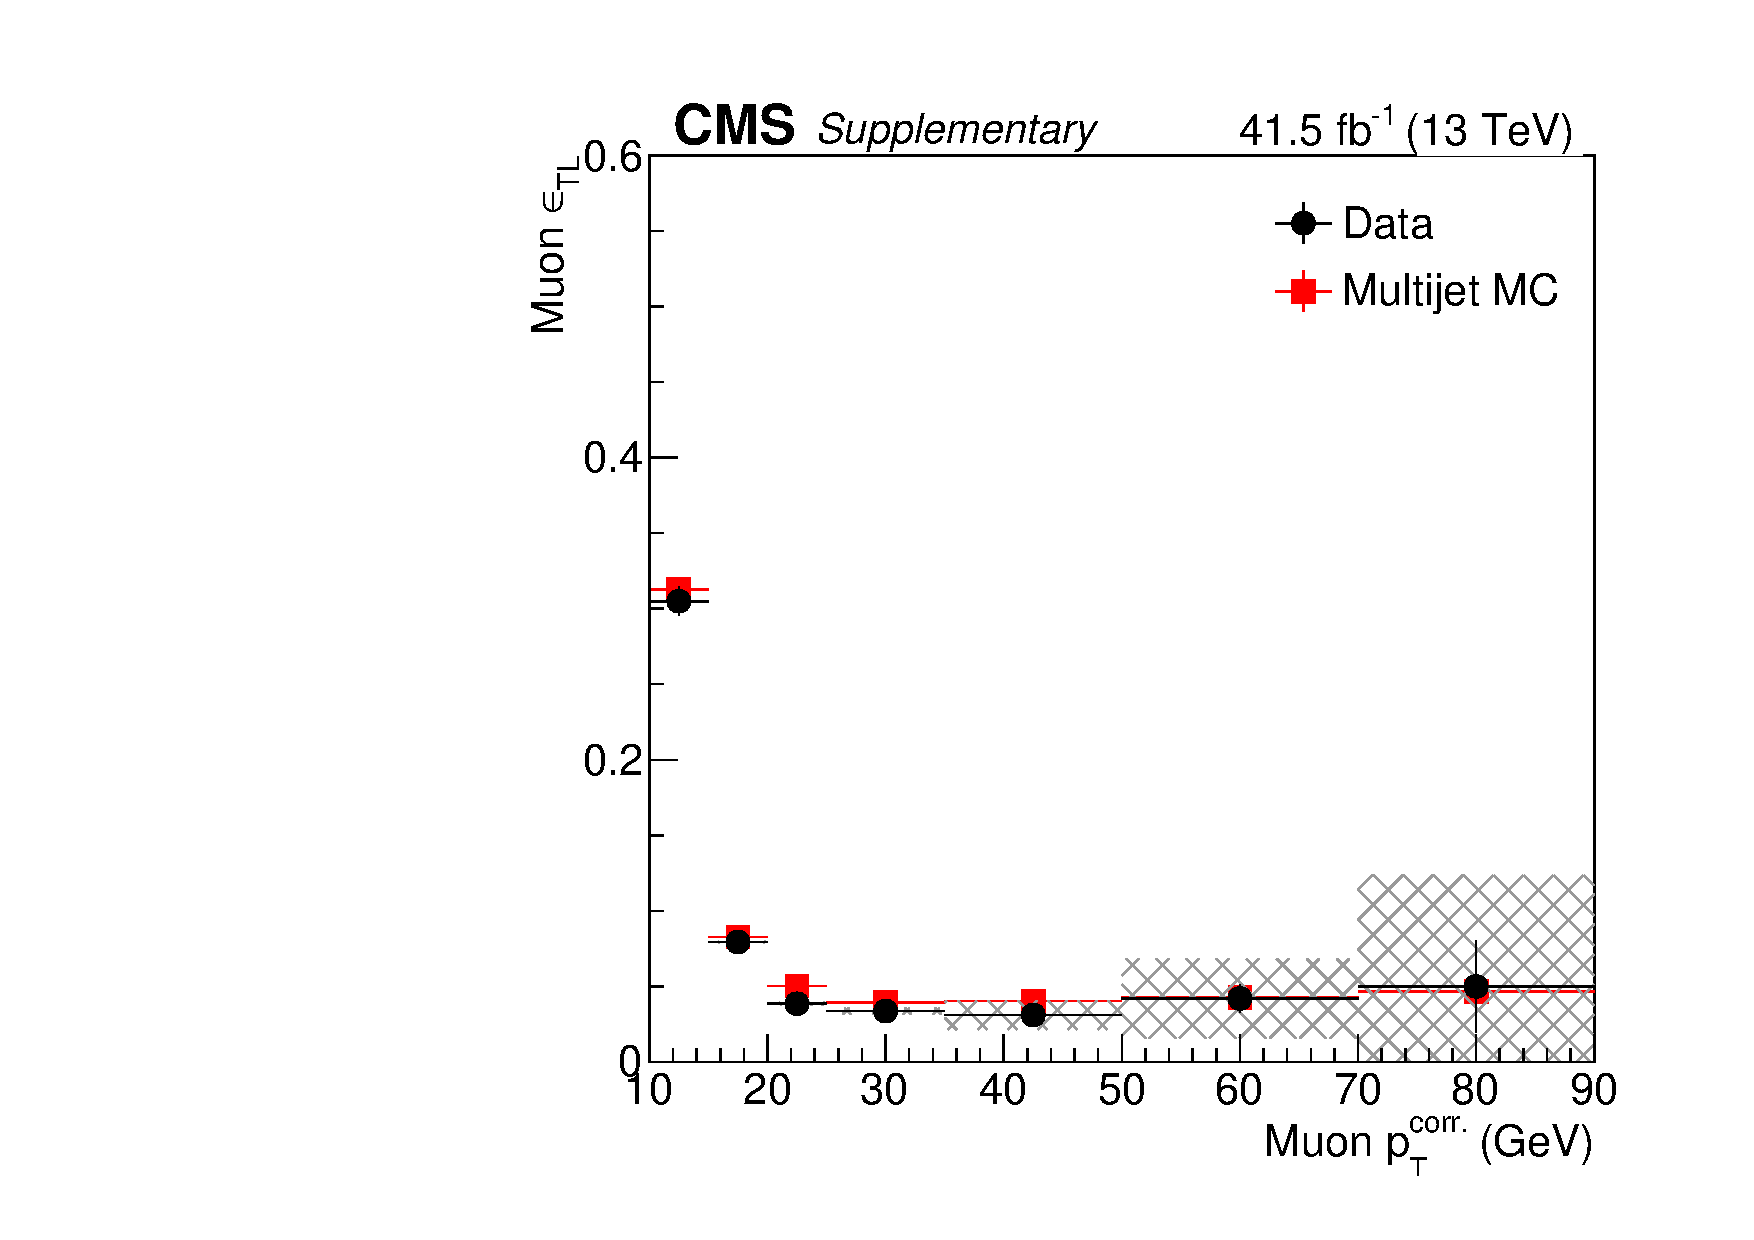
\includegraphics[width=.45\textwidth]{figs/ssan/fakerate/derivation/y2017/y2017_mu_1dfr_cone_LooseEMVA_IsoTrigs.pdf}
  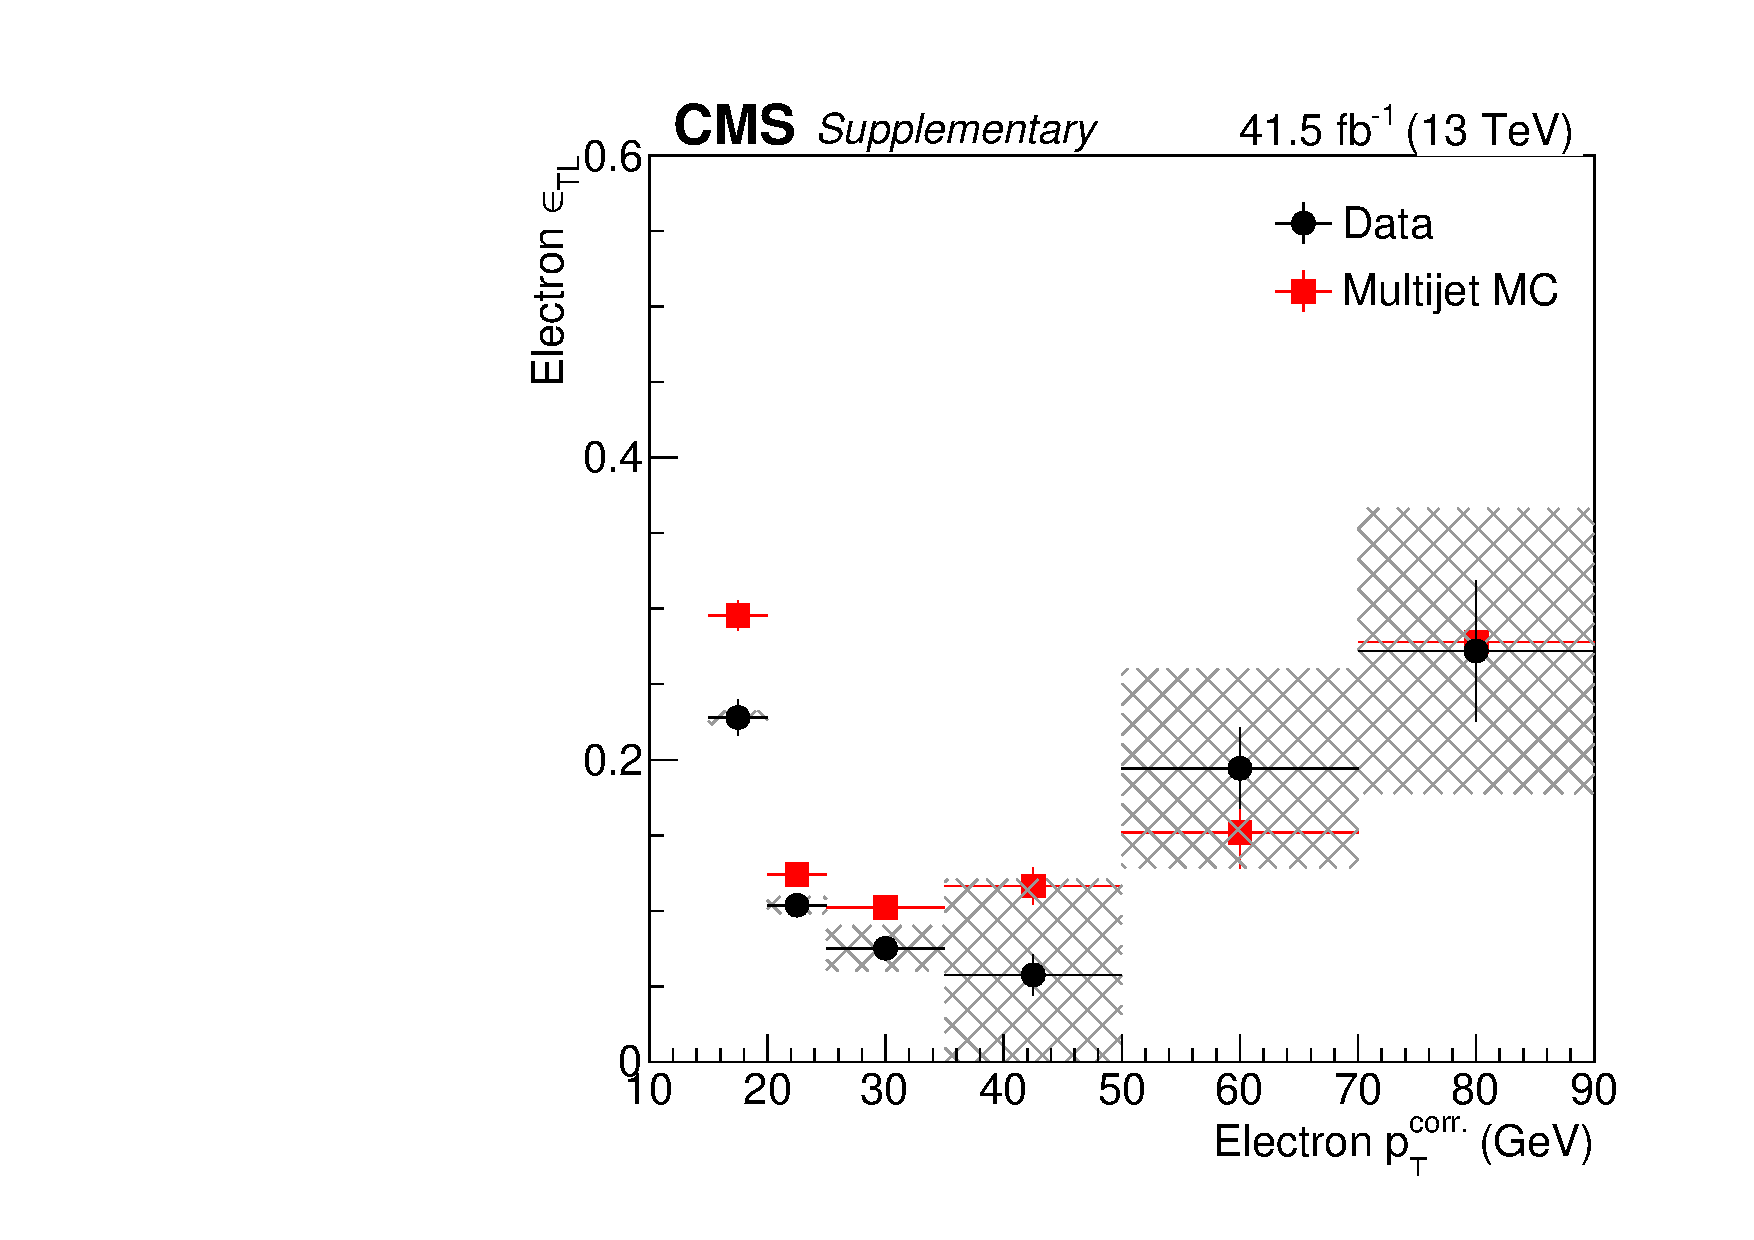
\includegraphics[width=.45\textwidth]{figs/ssan/fakerate/derivation/y2017/y2017_el_1dfr_cone_LooseEMVA_IsoTrigs.pdf} \\
  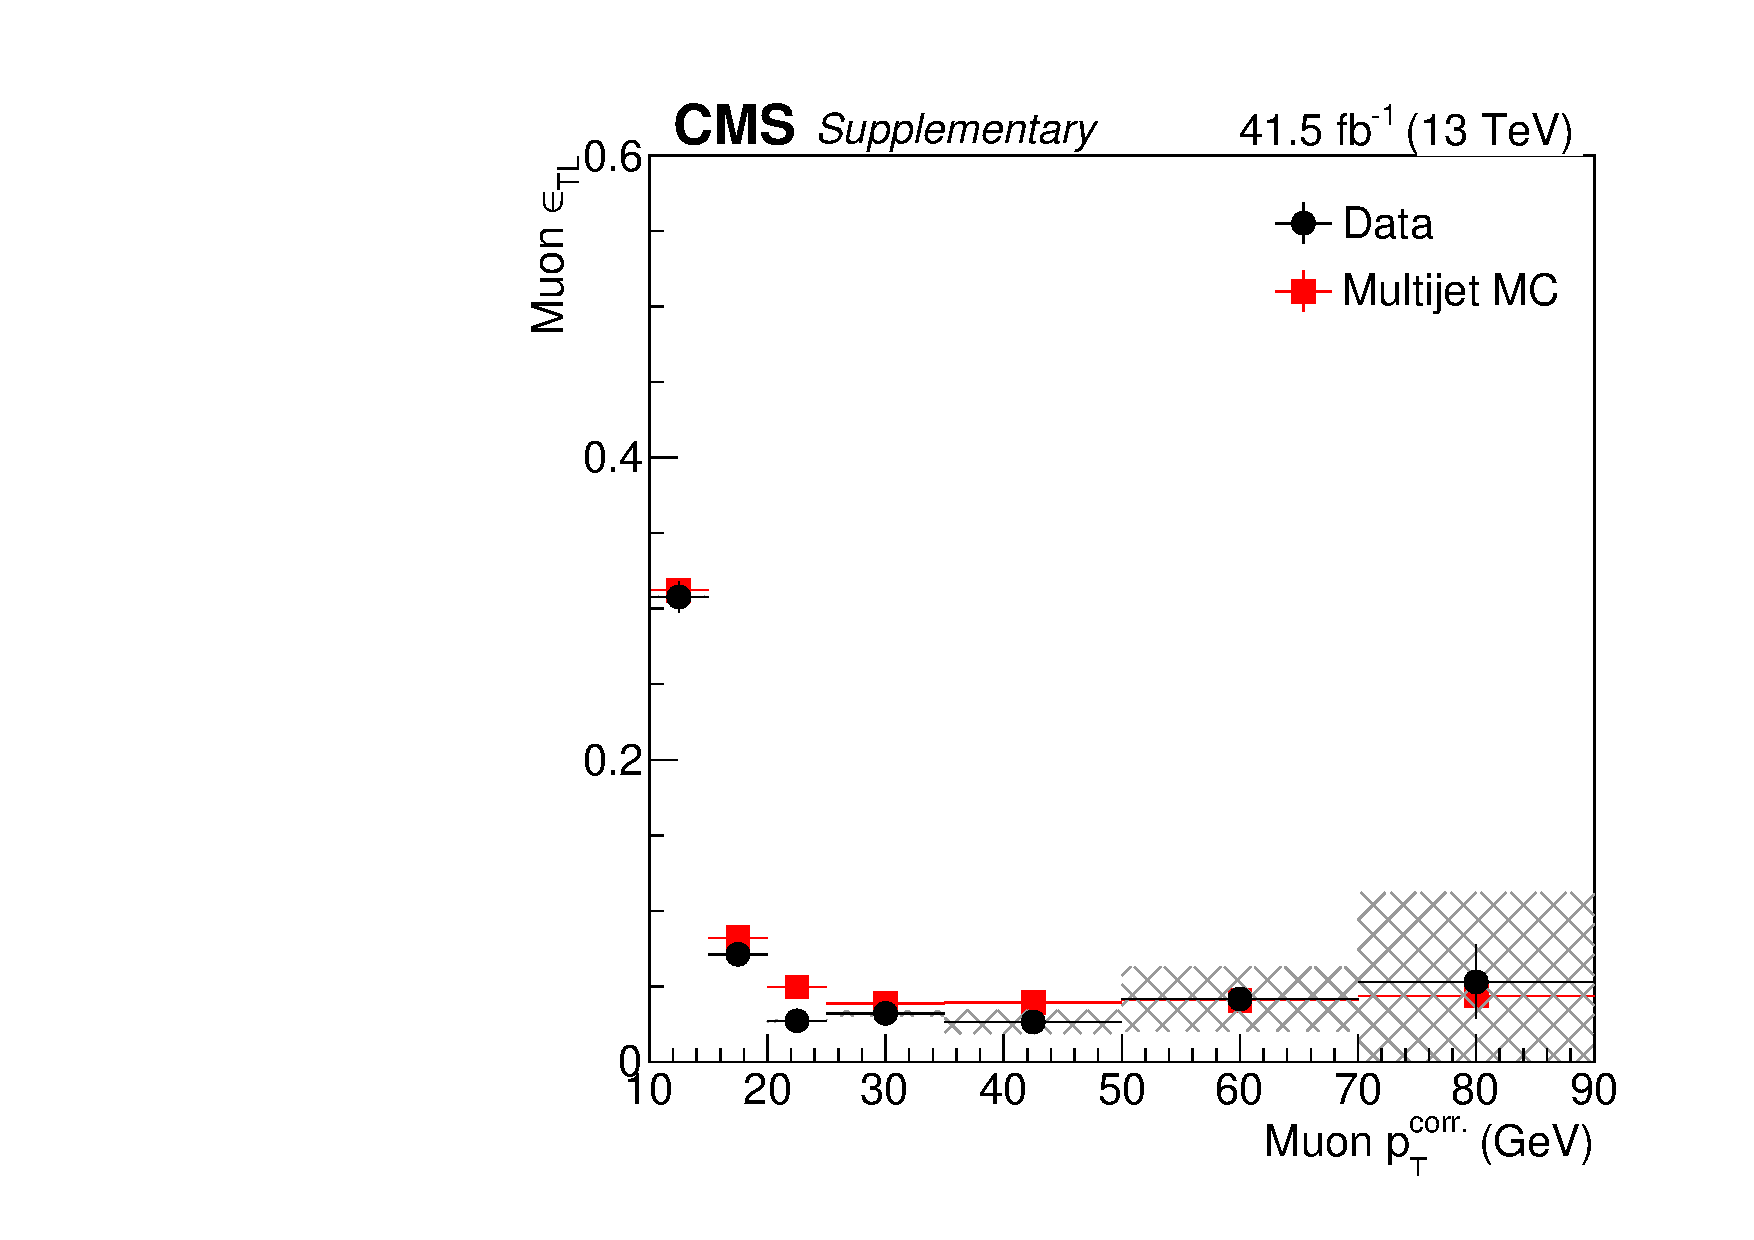
\includegraphics[width=.45\textwidth]{figs/ssan/fakerate/derivation/y2017/y2017_mu_1dfr_cone_LooseEMVA.pdf}
  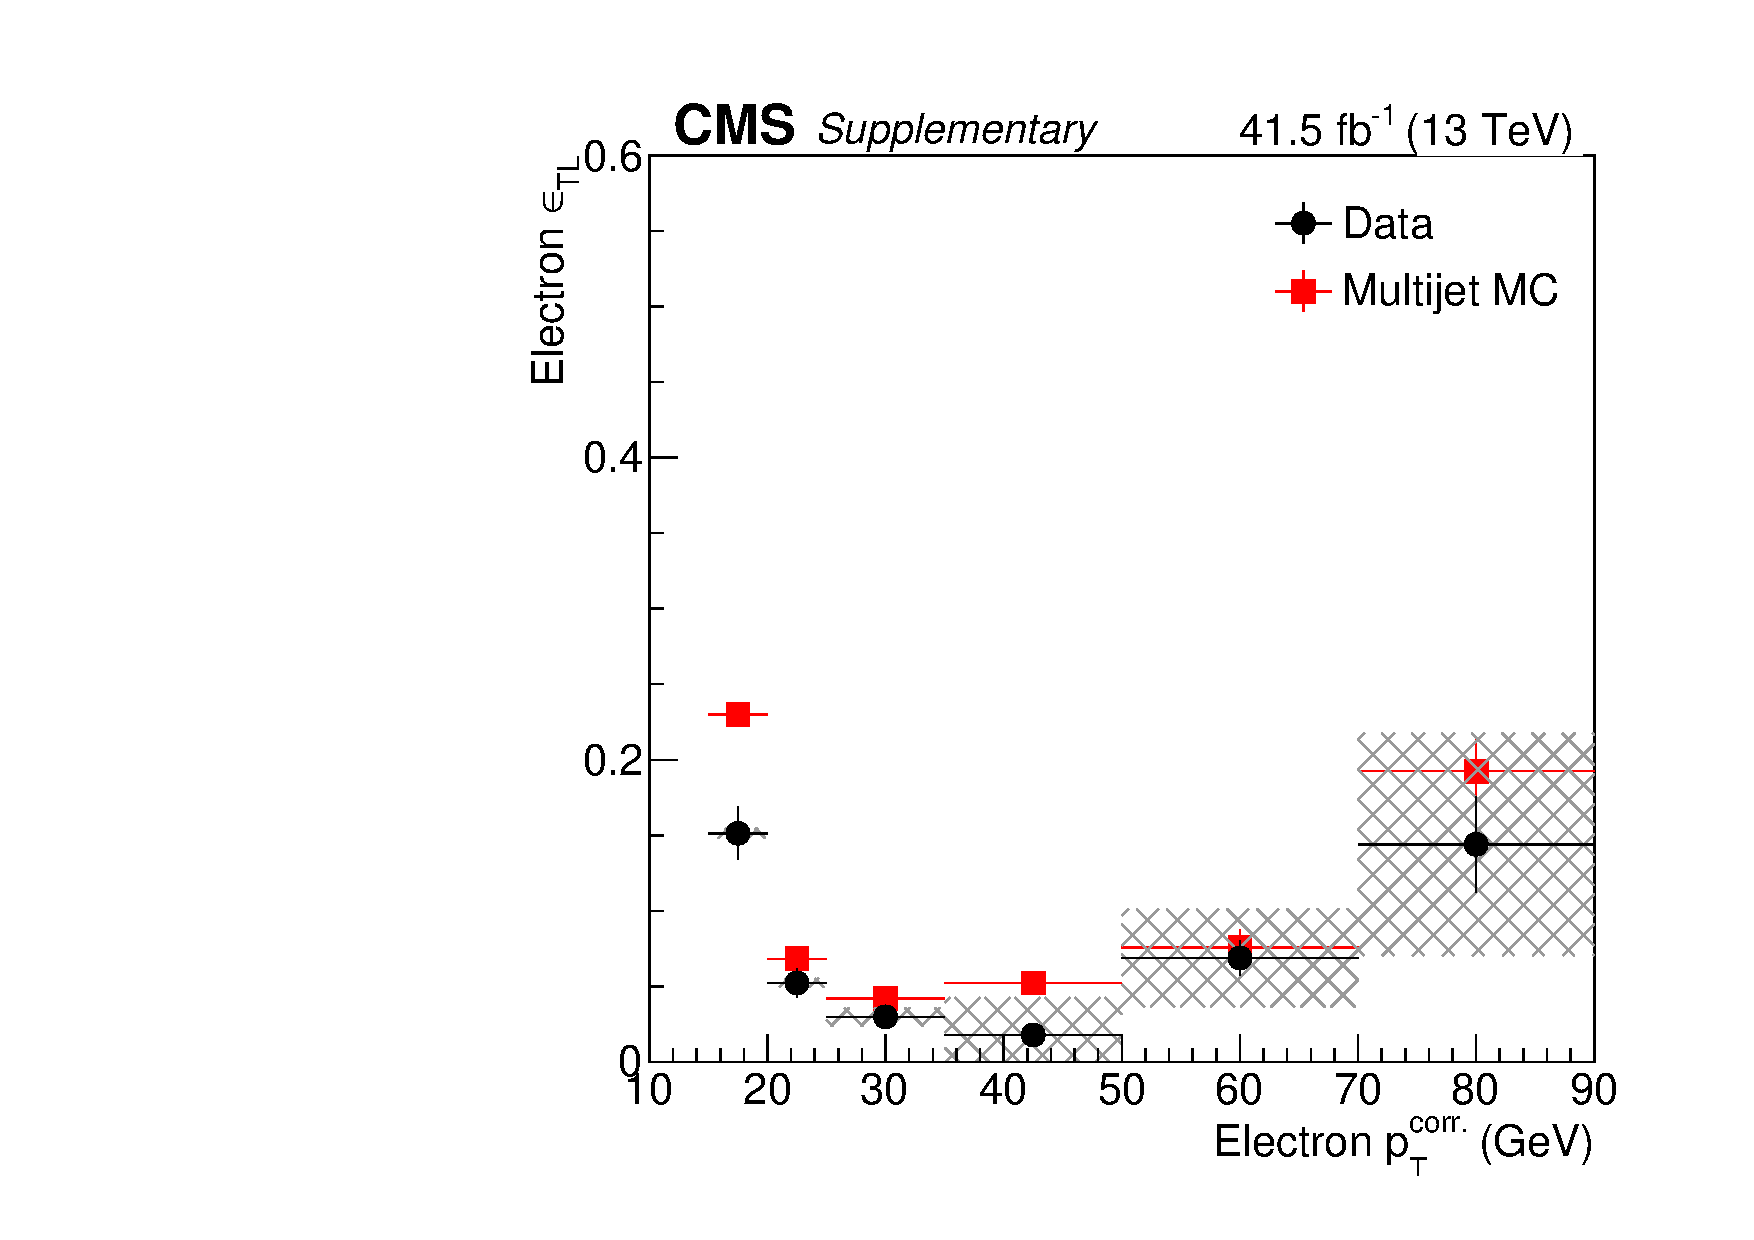
\includegraphics[width=.45\textwidth]{figs/ssan/fakerate/derivation/y2017/y2017_el_1dfr_cone_LooseEMVA.pdf}
  \caption{Electroweak contamination-corrected data fake rate projected vs \pt for 2017 data (black) and 2017 QCD simulation (red),
   for muons (left) and electrons (right). Isolated triggers are on top and non-isolated triggers on bottom.
      The shaded band in the projection is the systematic uncertainty related to the electroweak contamination.}
  \label{fig:QCDFRMuEle2017isoandnoniso}
  \end{figure}
  %%%%%%%%%%%%%%%%%%%%%%%%%%%%%%%%%%%%%%
  %%%%%%%%%%%%%%%%%%%%%%%%%%%%%%%%%%%%
  \begin{figure}[!hbtp]
  \centering
  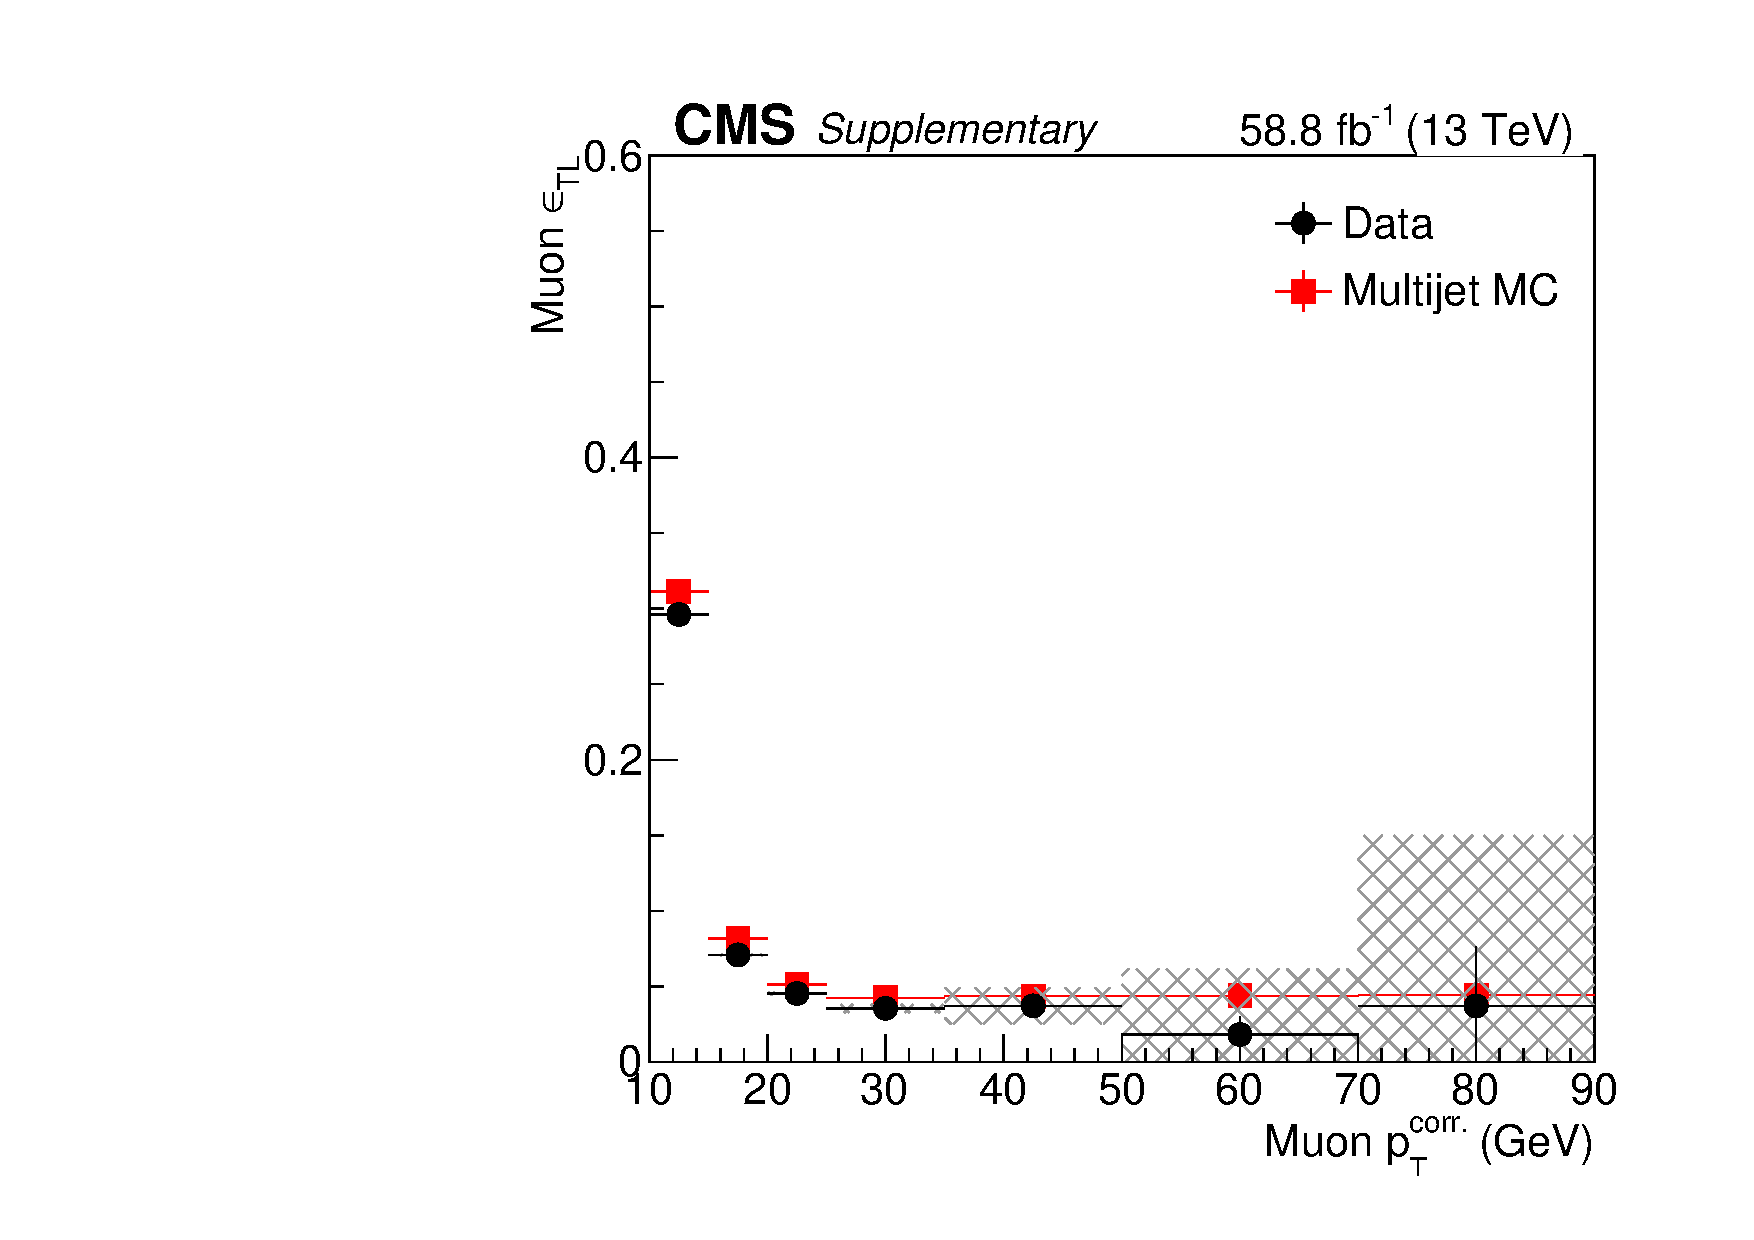
\includegraphics[width=.45\textwidth]{figs/ssan/fakerate/derivation/y2018/y2018_mu_1dfr_cone_LooseEMVA_IsoTrigs.pdf}
  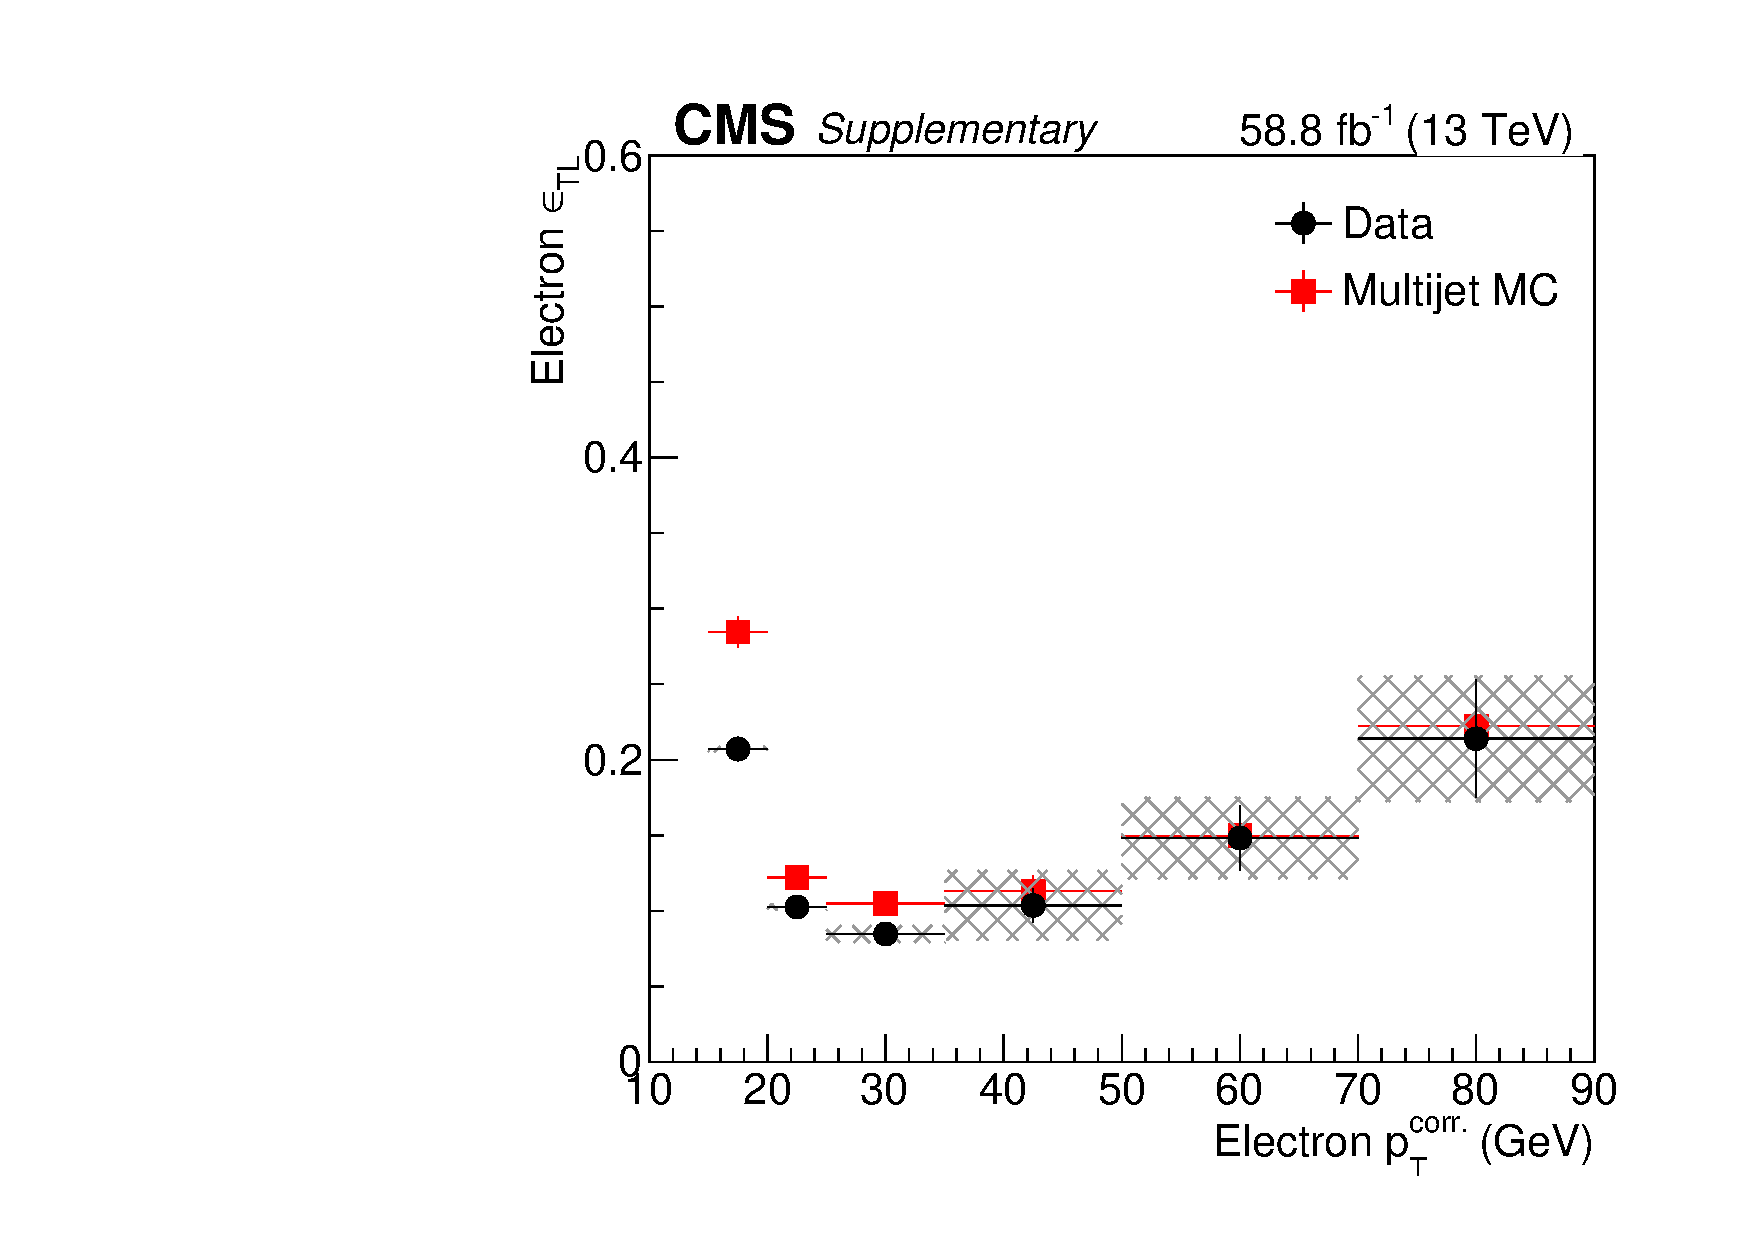
\includegraphics[width=.45\textwidth]{figs/ssan/fakerate/derivation/y2018/y2018_el_1dfr_cone_LooseEMVA_IsoTrigs.pdf} \\
  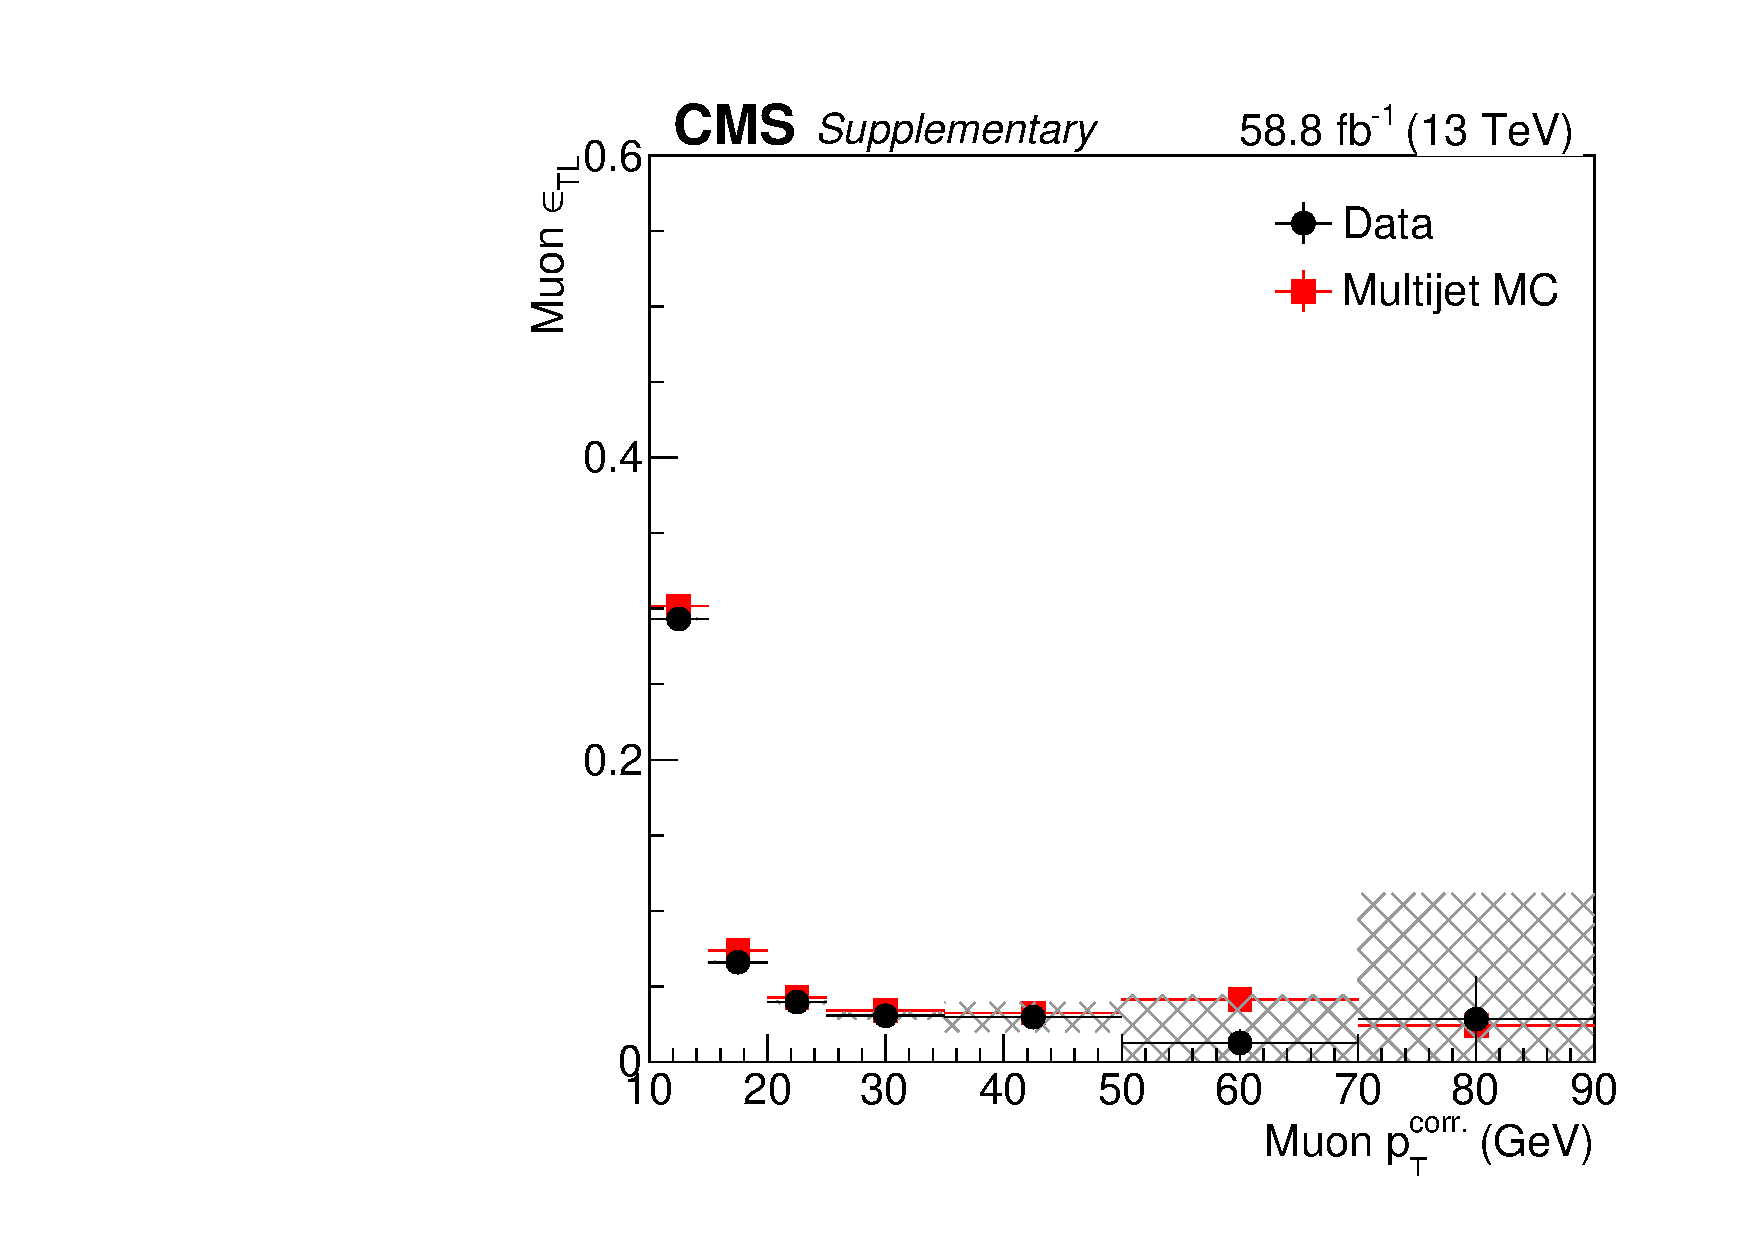
\includegraphics[width=.45\textwidth]{figs/ssan/fakerate/derivation/y2018/y2018_mu_1dfr_cone_LooseEMVA.pdf}
  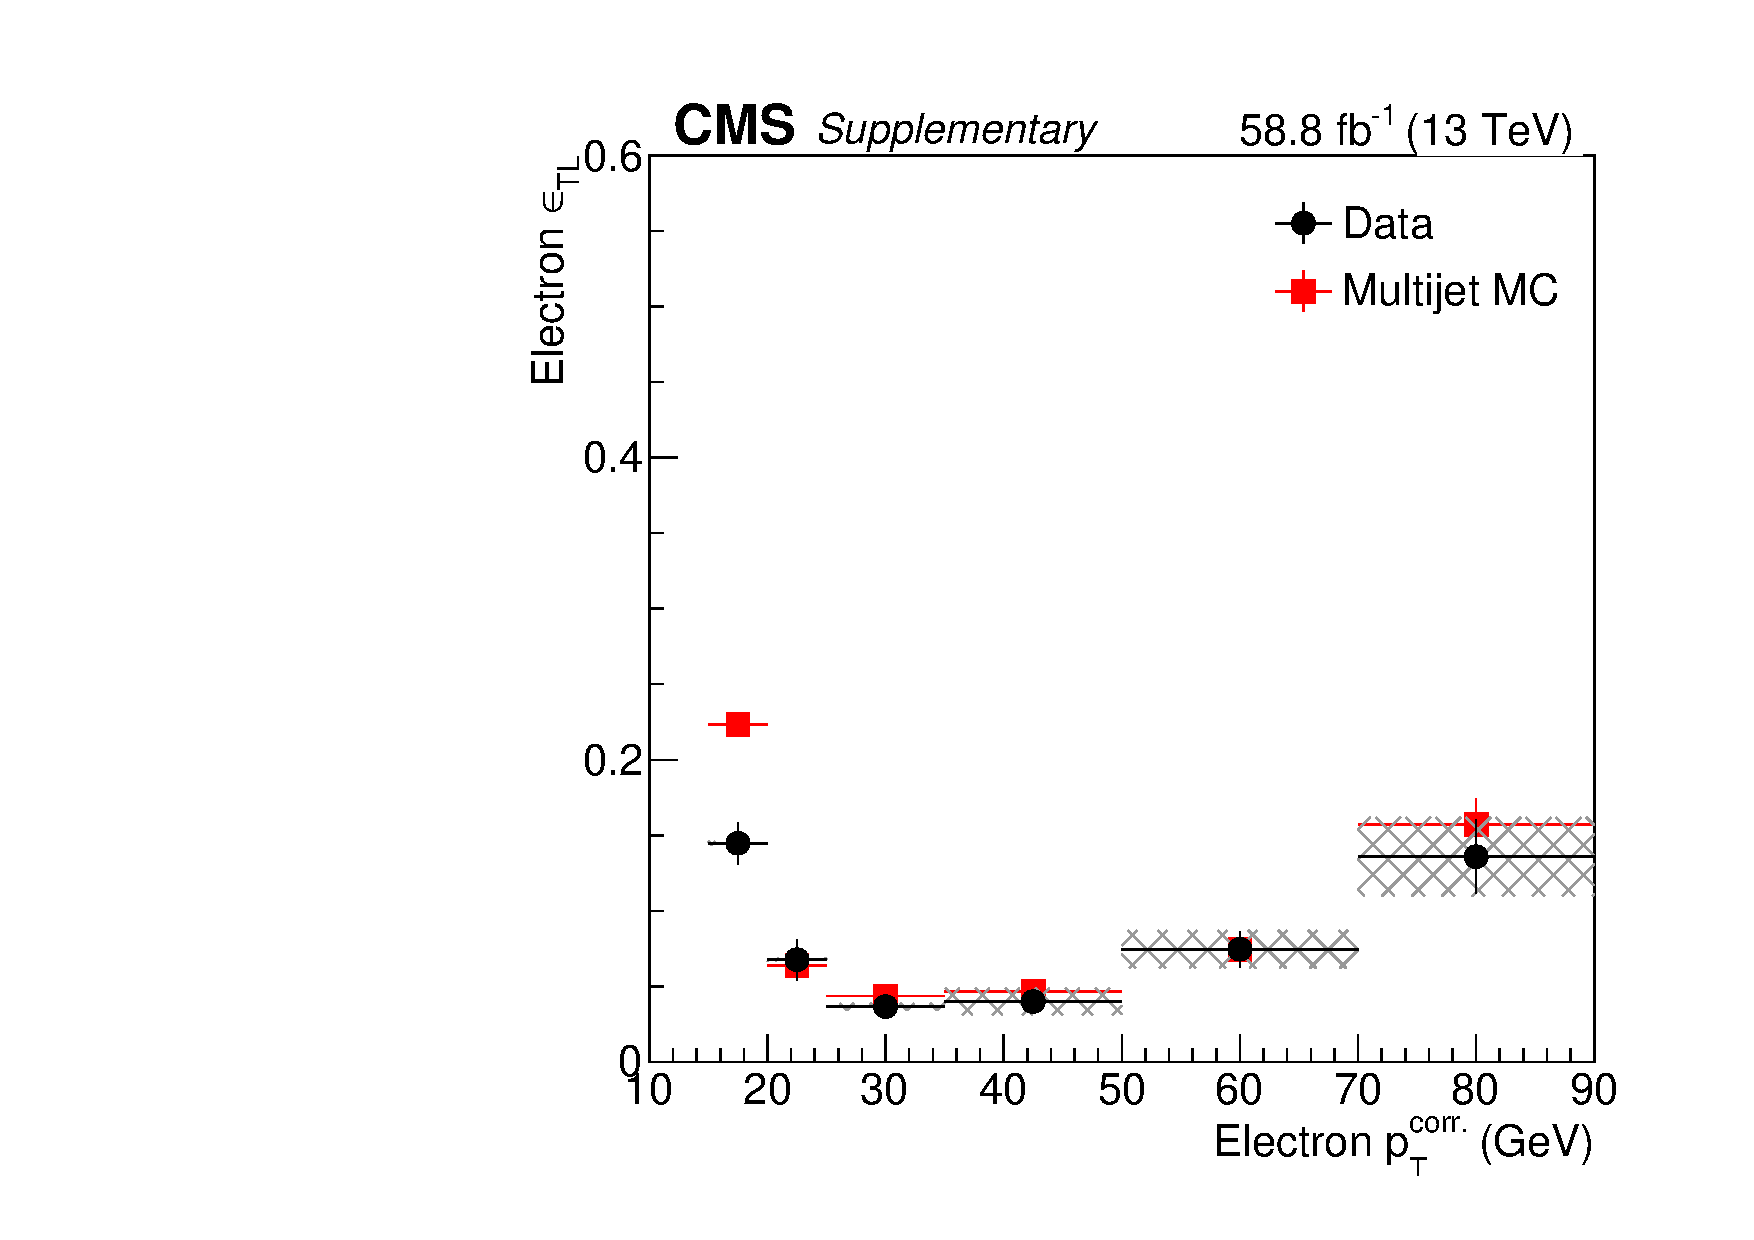
\includegraphics[width=.45\textwidth]{figs/ssan/fakerate/derivation/y2018/y2018_el_1dfr_cone_LooseEMVA.pdf}
  \caption{Electroweak contamination-corrected data fake rate projected vs \pt for 2018 data (black) and 2018 QCD simulation (red),
   for muons (left) and electrons (right). Isolated triggers are on top and non-isolated triggers on bottom.
      The shaded band in the projection is the systematic uncertainty related to the electroweak contamination.}
  \label{fig:QCDFRMuEle2018isoandnoniso}
  \end{figure}
  %%%%%%%%%%%%%%%%%%%%%%%%%%%%%%%%%%%%%%

\FloatBarrier

We test the closure of this method in simulation after making the inclusive
SUSY analysis baseline selection for various kinematic distributions in
\ref{fig:QCDFakesAll2017}. The filled histograms are events with one lepton
matched to a prompt lepton at generator lepton and another lepton not matched
to a prompt lepton (prompt-nonprompt events), separately for \ttjets and
\wjets simulation samples. The histogram with black points represents
application region events (one tight lepton and one loose-not-tight lepton,
at reconstruction-level) which are reweighted by the fake rate transfer
factor to form a prediction. The level of closure observed in the plots is
typically at 30\% or better, motivating a corresponding 30\% normalization
systematic uncertainty on the nonprompt lepton background.

\begin{figure}[!hbtp]
  \centering
  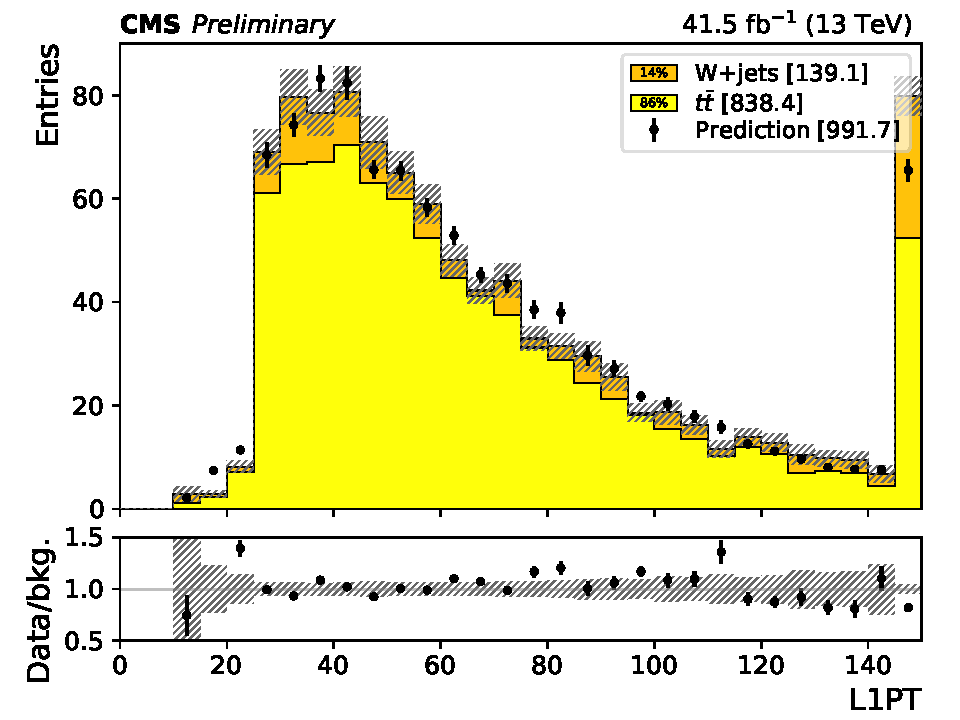
\includegraphics[width=.45\textwidth]{figs/ssan/fakerate/application/y2017/y2017_L1PT.pdf}
  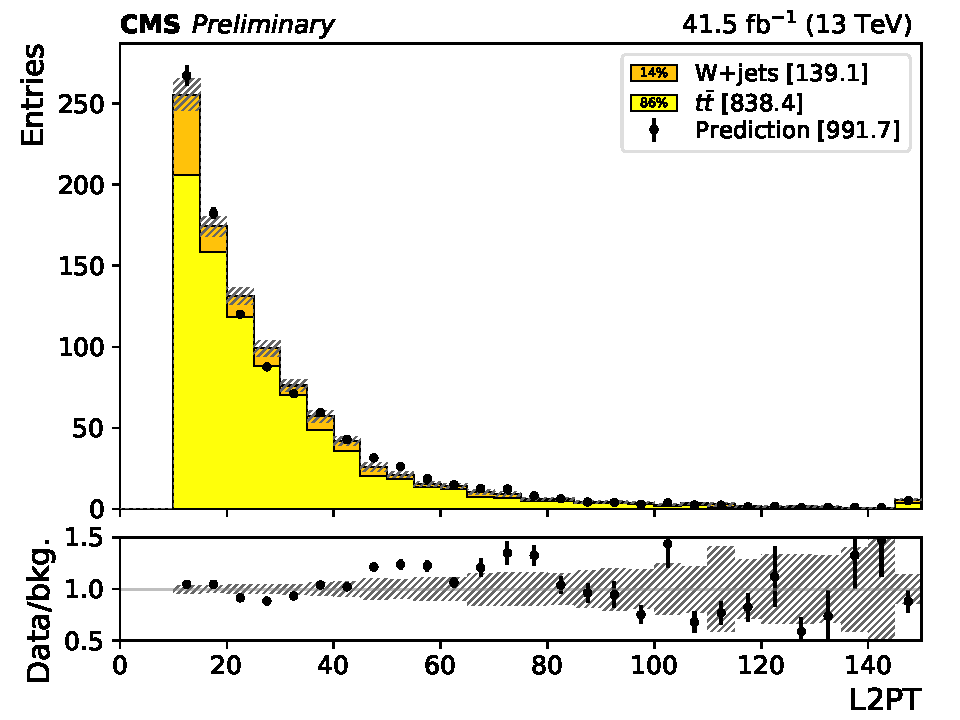
\includegraphics[width=.45\textwidth]{figs/ssan/fakerate/application/y2017/y2017_L2PT.pdf} \\
  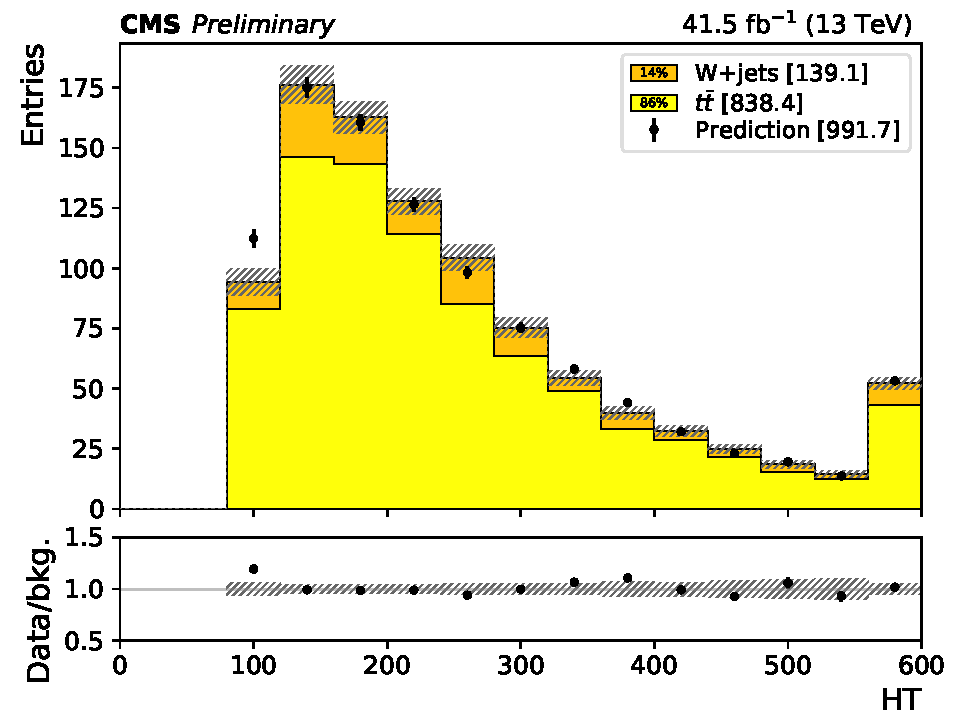
\includegraphics[width=.45\textwidth]{figs/ssan/fakerate/application/y2017/y2017_HT.pdf}
  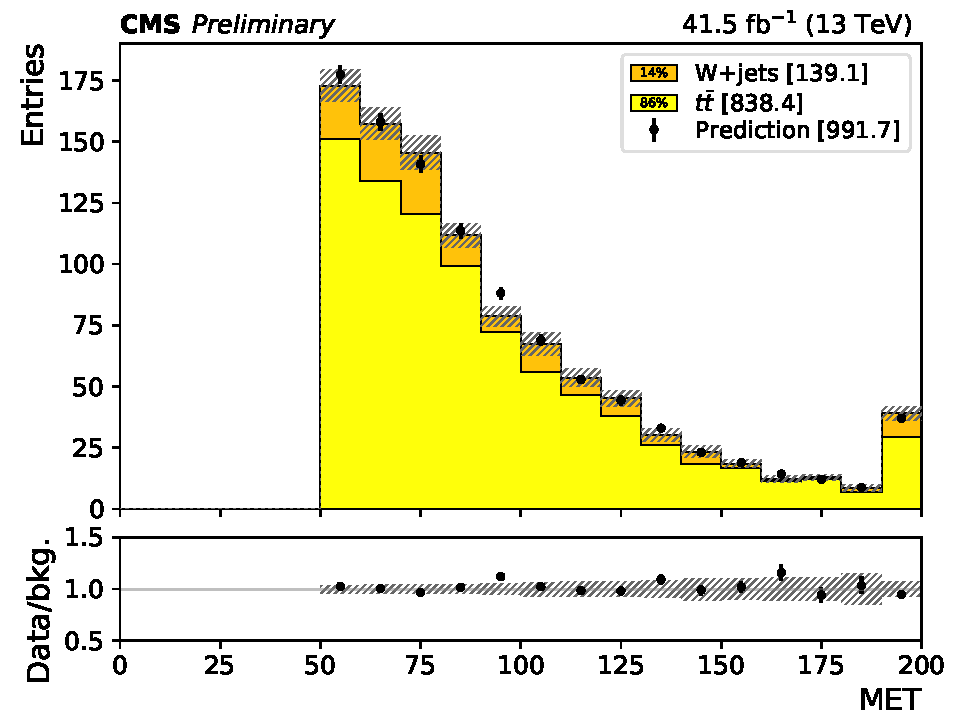
\includegraphics[width=.45\textwidth]{figs/ssan/fakerate/application/y2017/y2017_MET.pdf} \\
  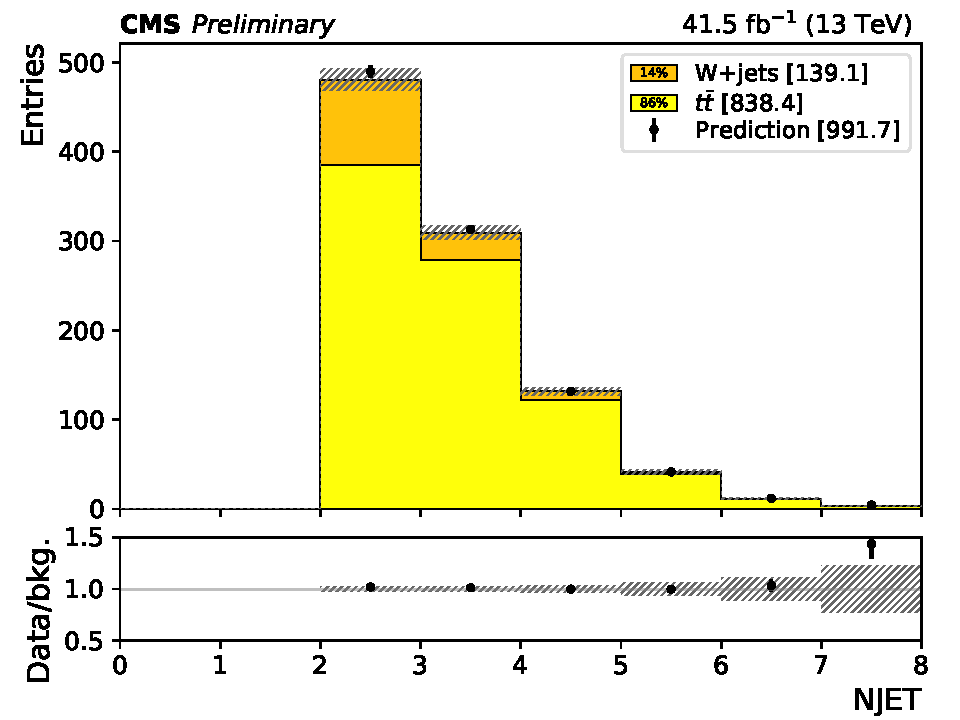
\includegraphics[width=.45\textwidth]{figs/ssan/fakerate/application/y2017/y2017_NJET.pdf}
  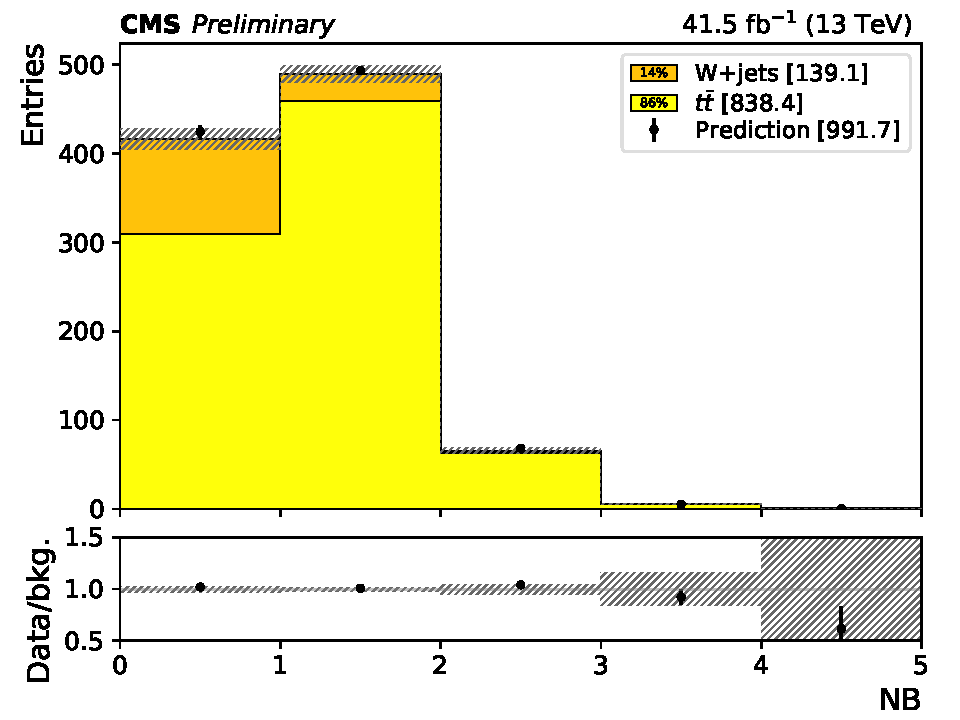
\includegraphics[width=.45\textwidth]{figs/ssan/fakerate/application/y2017/y2017_NB.pdf} \\
  \caption{ Electron+muon fake rate closure for QCD measurement in simulation.
  From left to right and top to bottom, the distributions are leading lepton \pt, subleading lepton \pt,
  \HT, \ptmiss, \Njets, and \Nbjets.}
  \label{fig:QCDFakesAll2017}
  \end{figure}

\FloatBarrier

\section{Charge misidentification}

The charge misidentification/flip background results from events that have
isolated OS leptons where the charge of one of the leptons is
misidentified due to mismeasurement (typical at high \pt) or bremsstrahlung.
Muons are relatively well-measured and less susceptible to radiation due to their
mass, so charge flips of muons are neglected compared to electrons.

The charge flip background is estimated by selecting OS $ee$ or $e\mu$ events 
which pass the appropriate baseline selection depending on analysis,
and then weighting the events by the \pt and $\eta$-dependent 
probability of electron charge mismeasurement, which is calculated from simulation.

The two-dimensional probability maps, shown for each of the three years of data collection 
in Fig.~\ref{fig:fliprate}, are obtained from a combination of
\ttbar and DY simulation. The probabilities
are then validated using a control sample in data of
SS $\PZ\rightarrow e^\pm e^\pm$ baseline events, 
instead using a $\ptmiss<50\GeV$ requirement to be
orthogonal to the signal regions. 
The level of disagreement in this control region
is used to assess the associated systematic uncertainty and to derive a
correction to the MC-based rate estimation.  In the 2016 data sample, we find good
agreement between prediction and data in the control region.
However, in the 2017 and 2018 data samples, the MC-based flip rate
is significantly lower than for
2016 due to the upgraded pixel detector (which added an extra inner pixel layer),
so the obsered number of events in the
SS $\PZ\rightarrow e^\pm e^\pm$ region is found to be nearly 40\% higher than the
predicted number of events. Consequently, the 2017 and 2018 charge
flip predictions are scaled up by approximately 40\%, as seen in
Figure~\ref{fig:flipclosure}. These year-by-year correction factors are summarized in
Table~\ref{tab:flipscaling}. Since we do not observe significant trends
in the lepton kinematics, we do not consider \pt and $\eta$-binned
corrections on top of the tabulated flat correction factors. 
In addition to the statistical uncertainties, we apply a 20\%
systematic uncertainty on this background prediction for all years. In MC, the
flip rate for muons is found to be an order of magnitude smaller than for
electrons and is therefore neglected, as it would in any case be covered by
the systematic uncertainty of 20\% on this background.



\begin{table}[h]
  \begin{center}
    \small
    \begin{tabular}{c|c}
      \hline
      year & observation/prediction \\
      \hline
        2016 & 1.01  \\
        2017 & 1.44  \\
        2018 & 1.41  \\
      \hline
    \end{tabular}
    \caption{ Ratio of observed flip rate in data to the flip rate prediction from simulation.
     These are the multiplicative correction to the MC-based charge flip probabilities. }
    \label{tab:flipscaling}
  \end{center}
\end{table}

\begin{figure}[!hbtp]
\centering
\centering
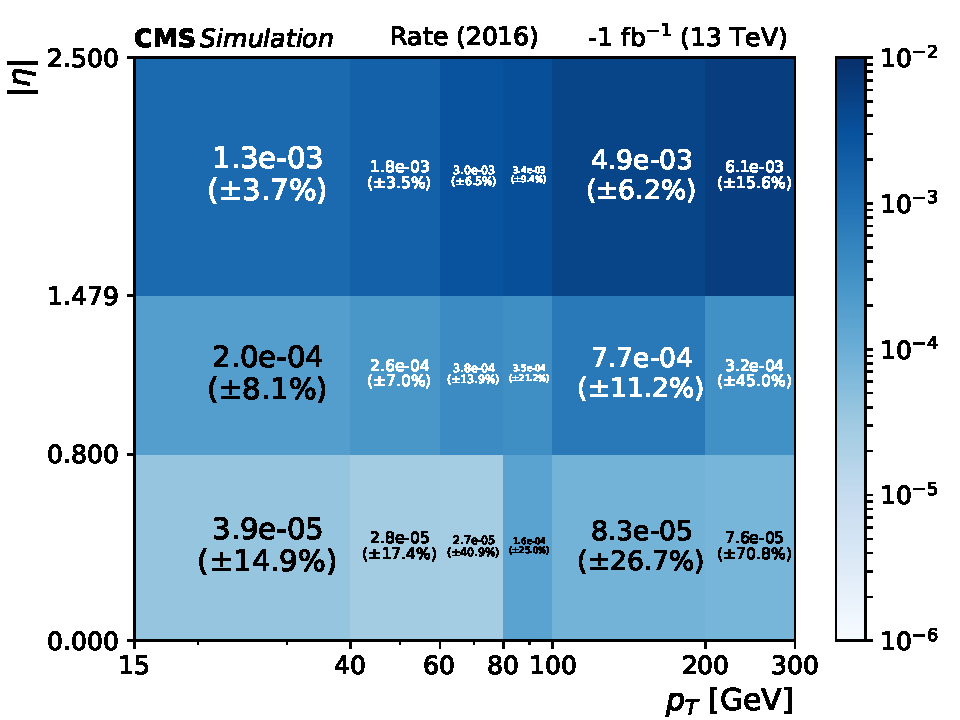
\includegraphics[width=.48\textwidth]{figs/ftan/flips/y2016/fliprate.pdf}
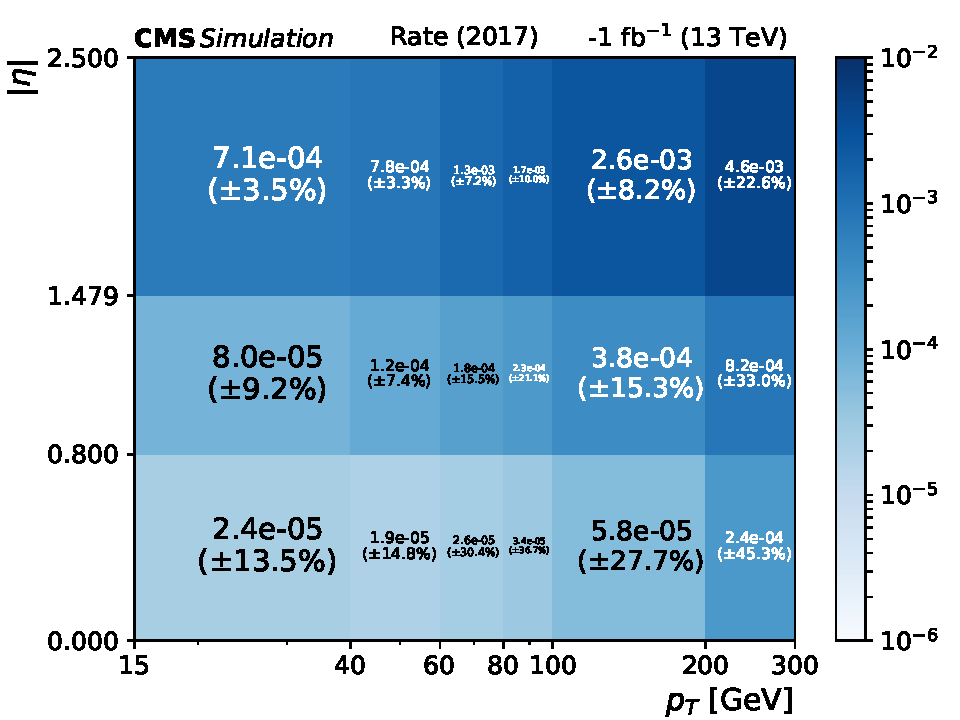
\includegraphics[width=.48\textwidth]{figs/ftan/flips/y2017/fliprate.pdf}
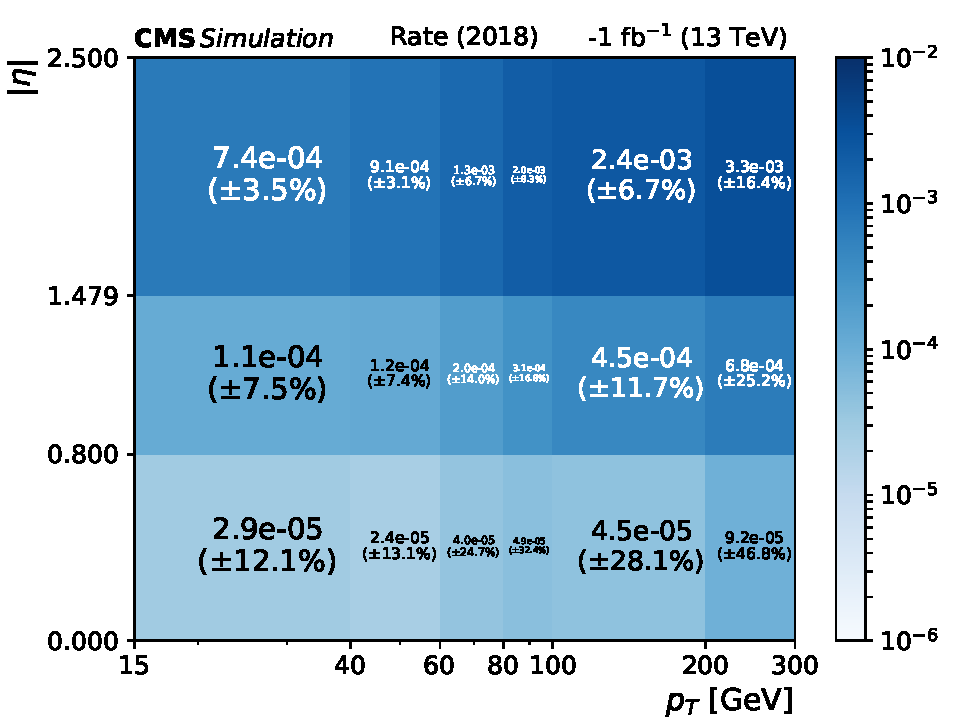
\includegraphics[width=.48\textwidth]{figs/ftan/flips/y2018/fliprate.pdf}
\caption{ Electron charge flip rate for 2016, 2017, and 2018. }
\label{fig:fliprate}
\end{figure}

\begin{figure}[!hbtp]
\centering
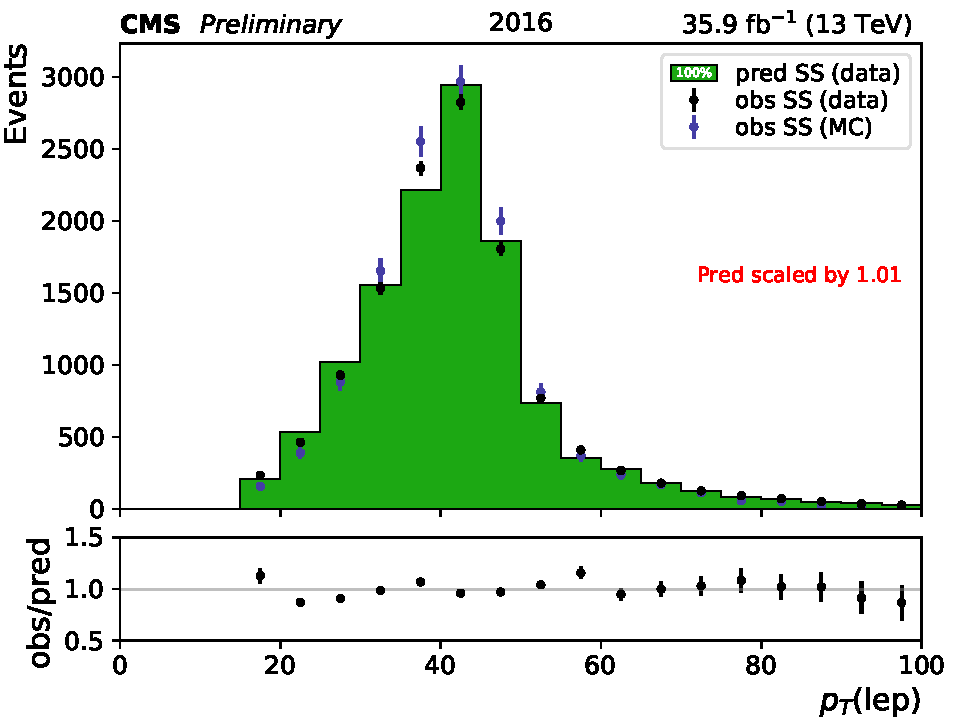
\includegraphics[width=.31\textwidth]{figs/ftan/flips/y2016/leppt.pdf}
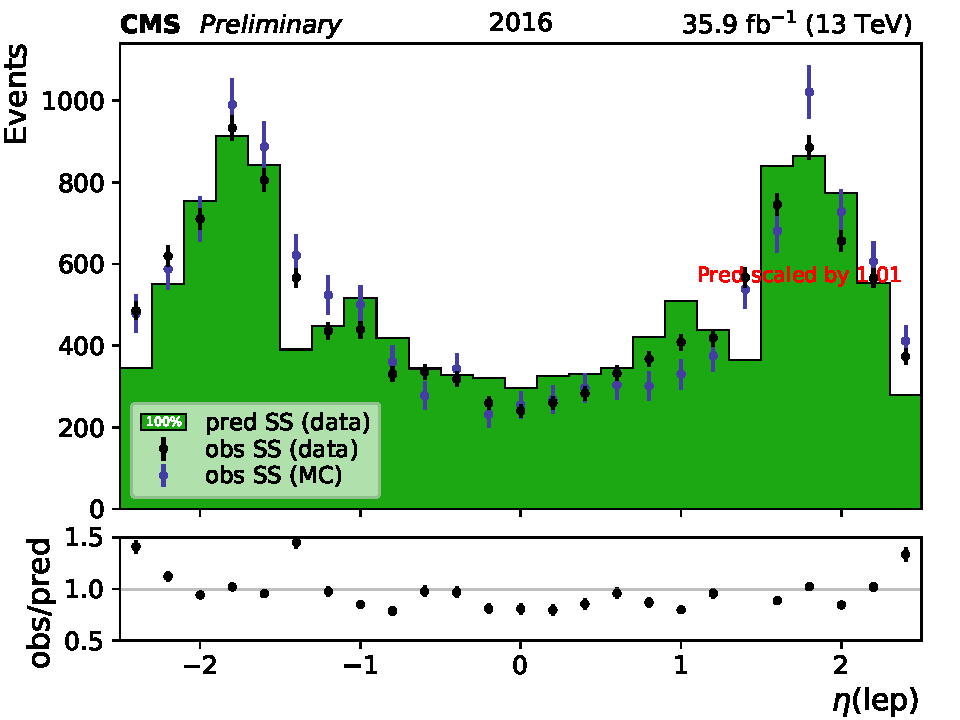
\includegraphics[width=.31\textwidth]{figs/ftan/flips/y2016/lepeta.pdf}
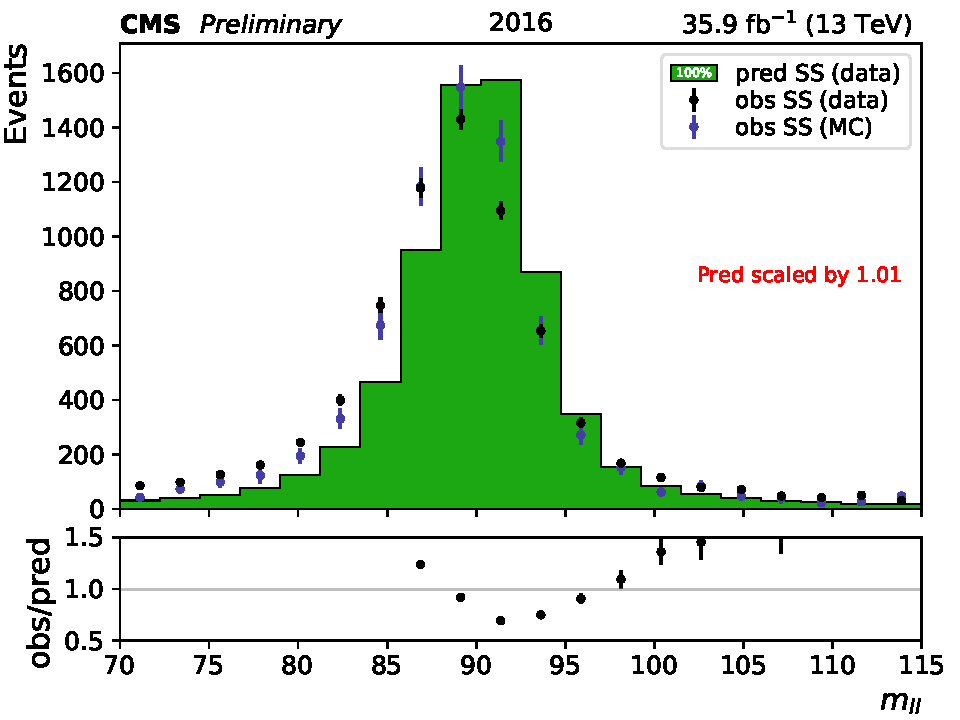
\includegraphics[width=.31\textwidth]{figs/ftan/flips/y2016/mll.pdf} \\
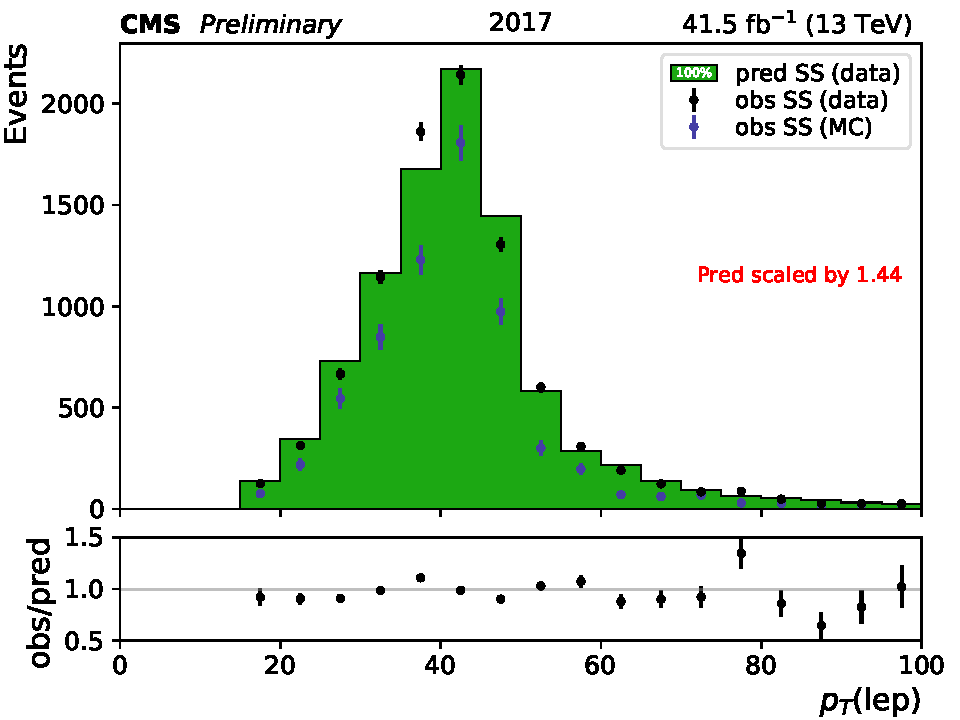
\includegraphics[width=.31\textwidth]{figs/ftan/flips/y2017/leppt.pdf}
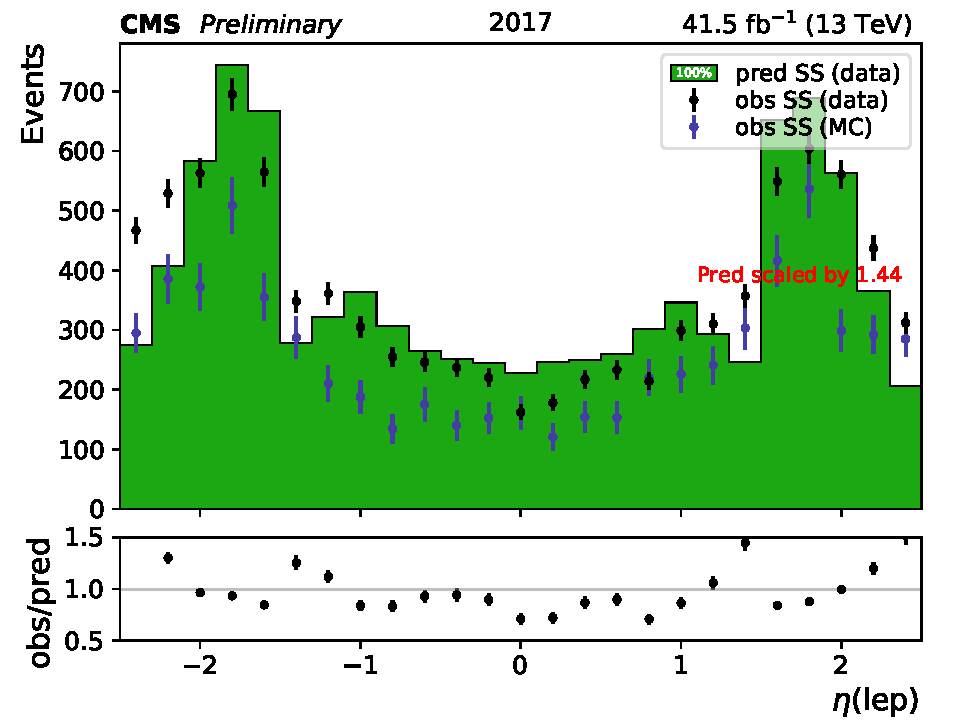
\includegraphics[width=.31\textwidth]{figs/ftan/flips/y2017/lepeta.pdf}
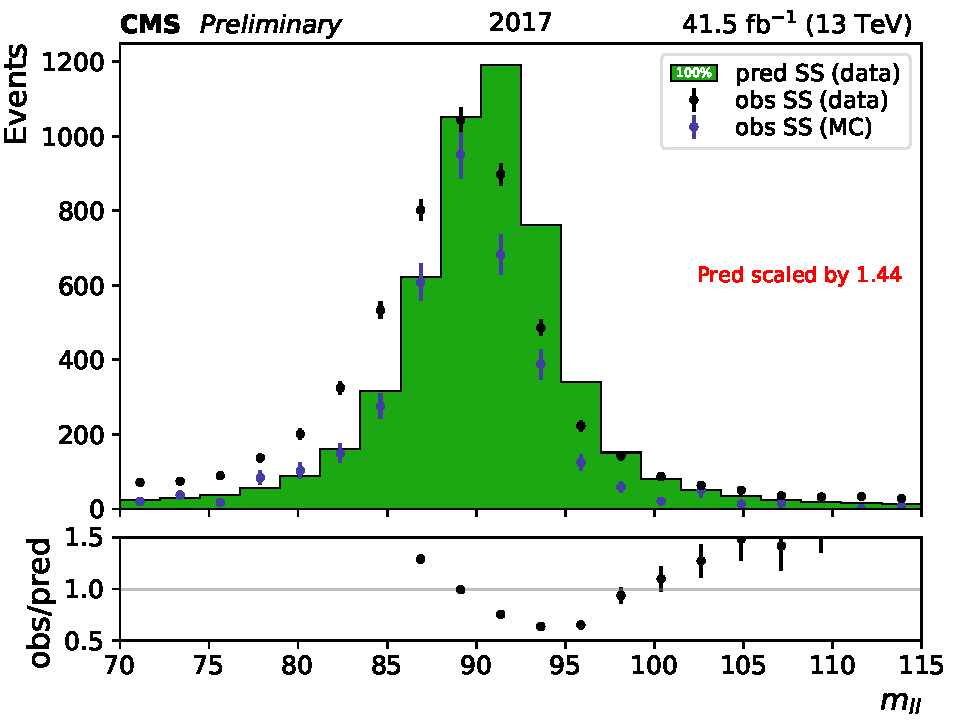
\includegraphics[width=.31\textwidth]{figs/ftan/flips/y2017/mll.pdf} \\
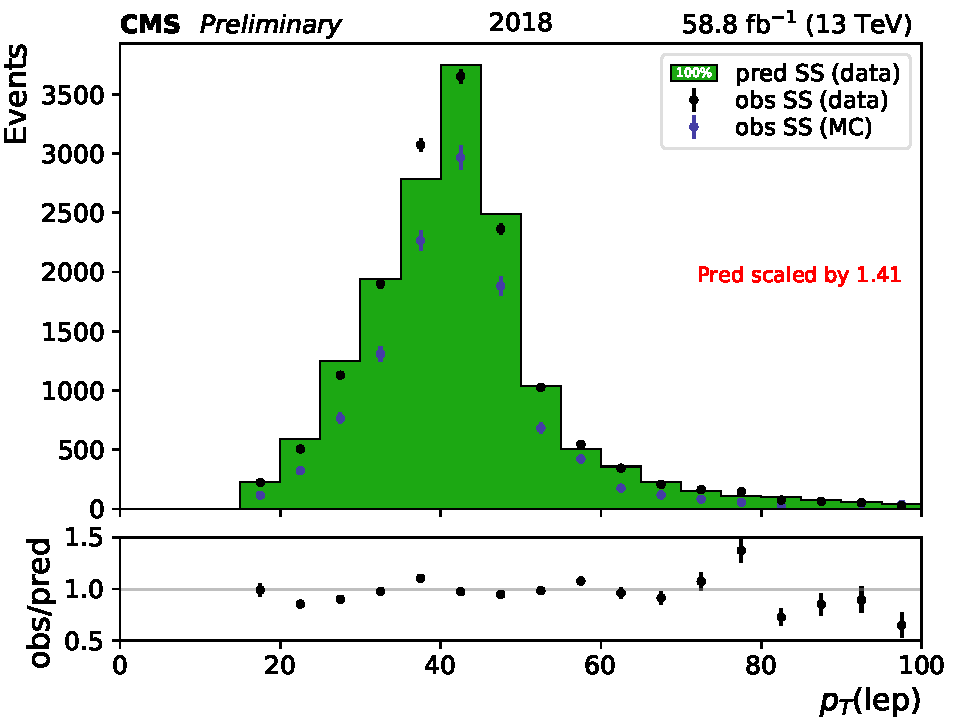
\includegraphics[width=.31\textwidth]{figs/ftan/flips/y2018/leppt.pdf}
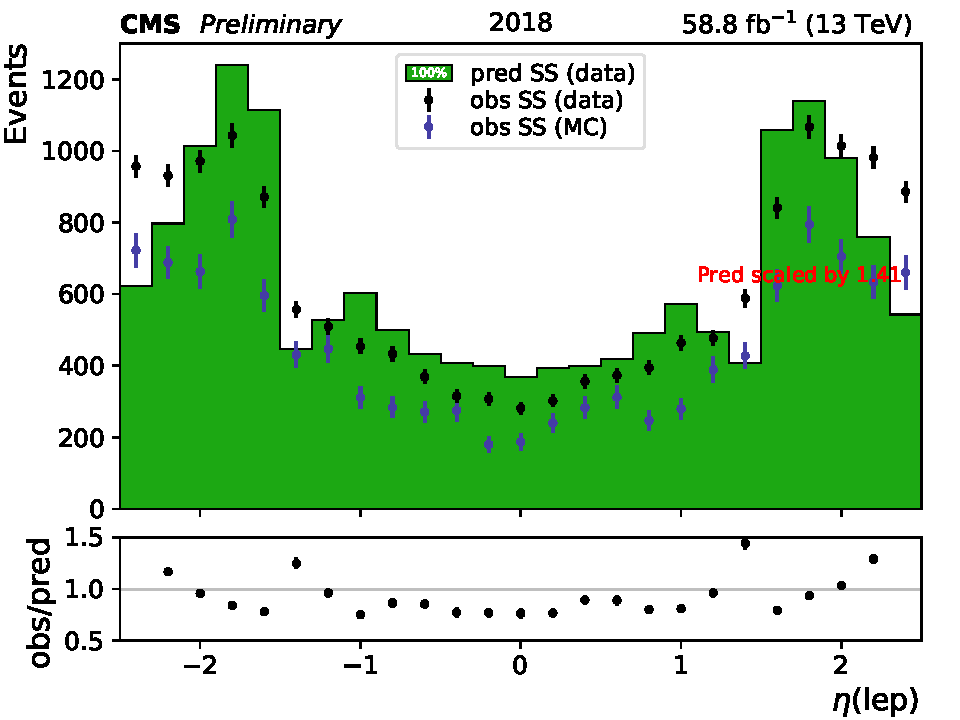
\includegraphics[width=.31\textwidth]{figs/ftan/flips/y2018/lepeta.pdf}
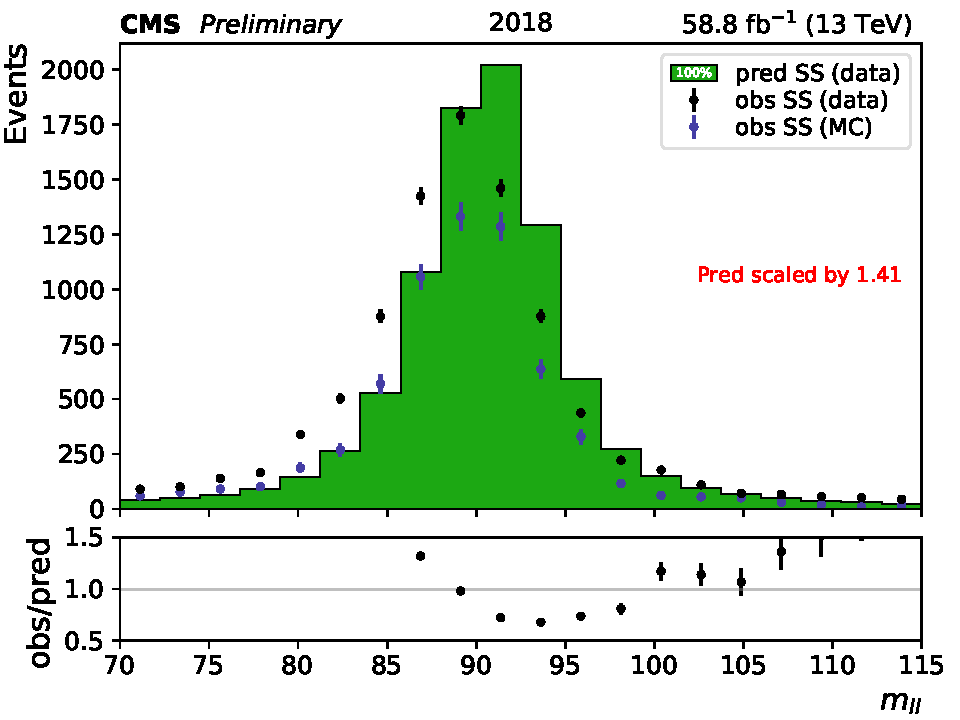
\includegraphics[width=.31\textwidth]{figs/ftan/flips/y2018/mll.pdf} \\
    \caption{  Predicted and observed lepton \pt (left) and $\eta$ (middle) and $m_{\ell\ell}$ (right) in a SS $\PZ \rightarrow e^\pm e^\pm$ peak
    for the years 2016, 2017, and 2018, from top to bottom.
The prediction is normalized to the observed data with the normalization factor inset in red.
The filled green histogram consists of predicted charge flip events (reweighted OS events),
the black points consist of observed charge flip events in data (SS), and the blue points
show the observed charge flip events in MC (SS).
}
\label{fig:flipclosure}
\end{figure}

\FloatBarrier

\section{Corrections}

In addition to corrections associated with JEC, \PQb-tagging, lepton scale factors,
and trigger scale factors, mentioned throughout previous sections and chapters, we
apply two more dedicated corrections to simulation to bring better agreement between data
and simulation. Both corrections deal with \Njets and \Nbjets for the
\ttW, \ttZ, and \ttH processes,
whose distributions need to be estimated correctly at high multiplicities,
which is especially important for the SM \tttt analysis, as these are
the leading background processes.


\subsection{Gluon splitting}

The \ttW, \ttZ, and \ttH processes need an additional source of \cPqb quarks
in order to populate the $\Nbjets\geq 3$ bins of the SM \tttt analysis, as
they should only have up to 2 hard \cPqb jets from the \ttbar decay.
If simulation does not model the gluon splitting process $g\rightarrow \bbbar$,
the contributions in these high \Nbjets bins can be drastically wrong.
In fact, Ref.~\cite{CMS:ttbb} measures that the ratio of cross sections
of $\ttbar\bbbar$ to $\ttbar jj$ is about $1.7\pm0.6$ times as high in data
compared to simulation. As a result, events with additional \cPqb quarks
in these three background processes are scaled up by a factor of 
$1.7\pm0.6$ and the uncertainty is translated into
a systematic uncertainty affecting analysis results. 

\subsection{ISR/FSR jet multiplicity}

Similarly, \ttW and \ttZ processes need an additional source of jets
in order to populate the $\Njets \geq 4$ bins of the analyses.
To improve on the modeling of the
multiplicity of additional jets from initial-state radiation (ISR) and
final-state radiation (FSR) in MadGraph,
\ttW and \ttZ MC events are reweighted based on the
number of ISR or FSR jets ($\Njets^{\rm ISR/FSR}$).
The \ttH process is not considered for this reweighting as
the $\PH\rightarrow \PW\PW^*$ decay will result in extra jets from one
of the \PW bosons.

The reweighting method, developed in Ref.~\cite{CMS:isrweight} for 2016
simulation samples, is based on the Data/MC ratio in the light-flavor jet
multiplicity in dilepton \ttbar events (using MadGraph MC), as shown in
Figure~\ref{fig:isrweight2} for the 2017 and 2018 simulation samples. The
method requires exactly two b-tagged jets, and assumes that all other jets
are ISR or FSR. The reweighting factors vary within the range of
$[0.77,1.46]$ for $\Njets^{\rm ISR/FSR}$ between 1 and 4. The corresponding
Data/MC ratios are shown in Figure~\ref{fig:isrweight2}, where the different
plots are based on different number of partons simulated at the matrix
element. 

We take one half of the deviation from unity as the systematic
uncertainty in these reweighting factors.
The size of the systematic comes from deviations observed in an orthogonal
single-lepton channel. We make a tight single-lepton selection with tight
lepton $\pt>25\GeV$, $\ptmiss>50\GeV$, $\HT>300\GeV$, and 2 \PQb tagged jets. 
The simulation is normalized to data to account for trigger and lepton efficiencies.
Figure~\ref{fig:isrweightsyst} shows the jet multiplicity distribution for 2018 data/MC before and after
applying the 2018-derived reweighting factors. The systematic uncertainty of half of the deviation from unity covers
variations present in the reweighted single lepton jet multiplicity distributions.

  \begin{figure}[h!]
  \centering
  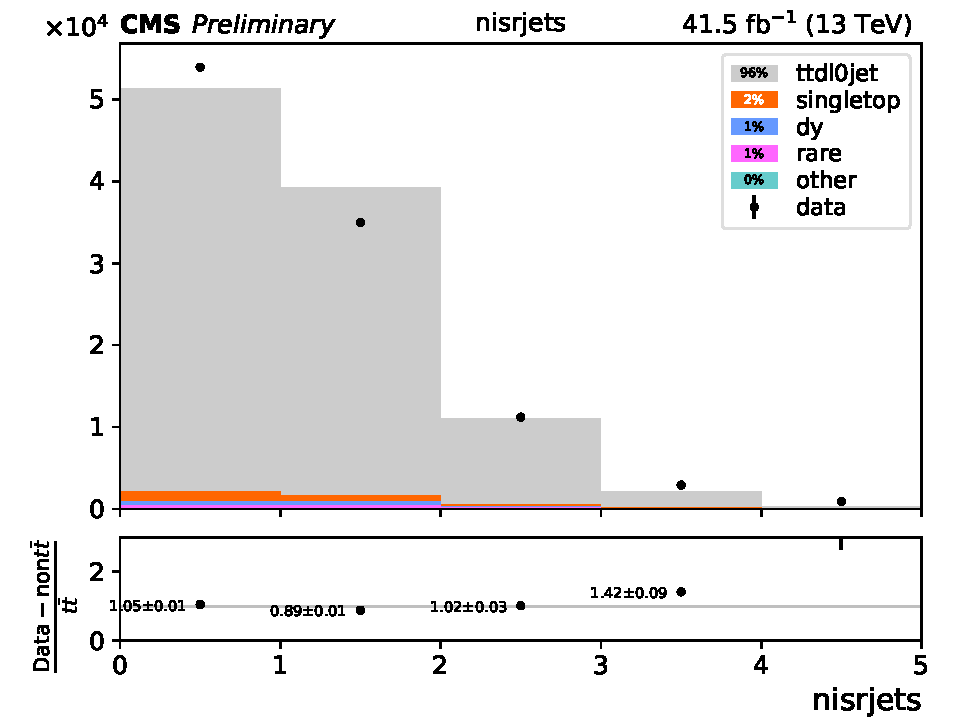
\includegraphics[width=0.48\textwidth]{figs/ftan/isr/y2017_isrrw_nisrjets0.pdf}
  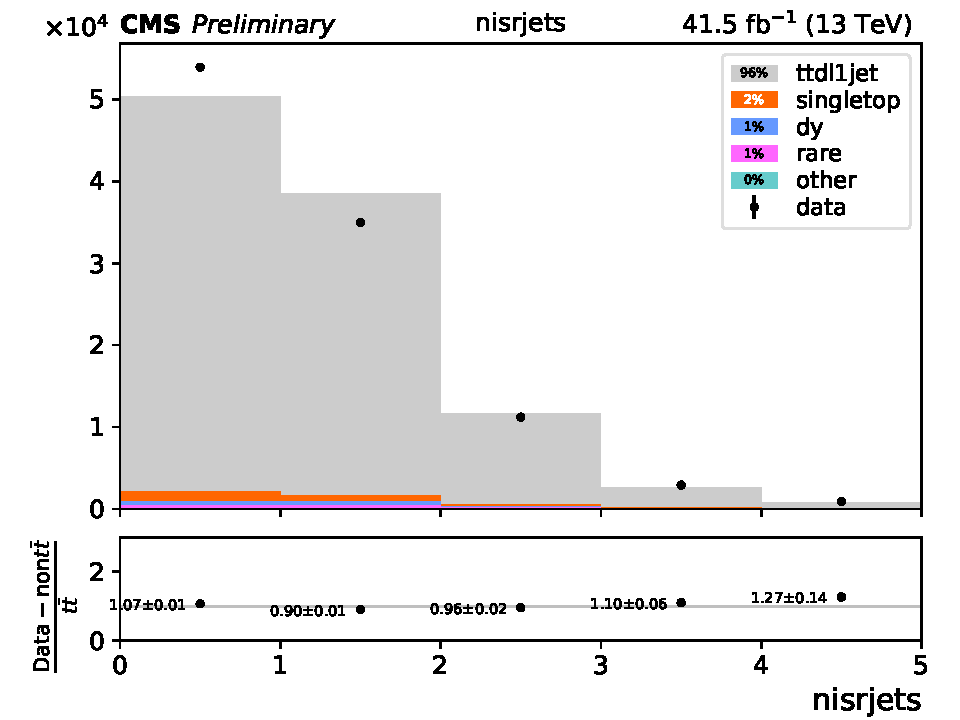
\includegraphics[width=0.48\textwidth]{figs/ftan/isr/y2017_isrrw_nisrjets1.pdf} \\
  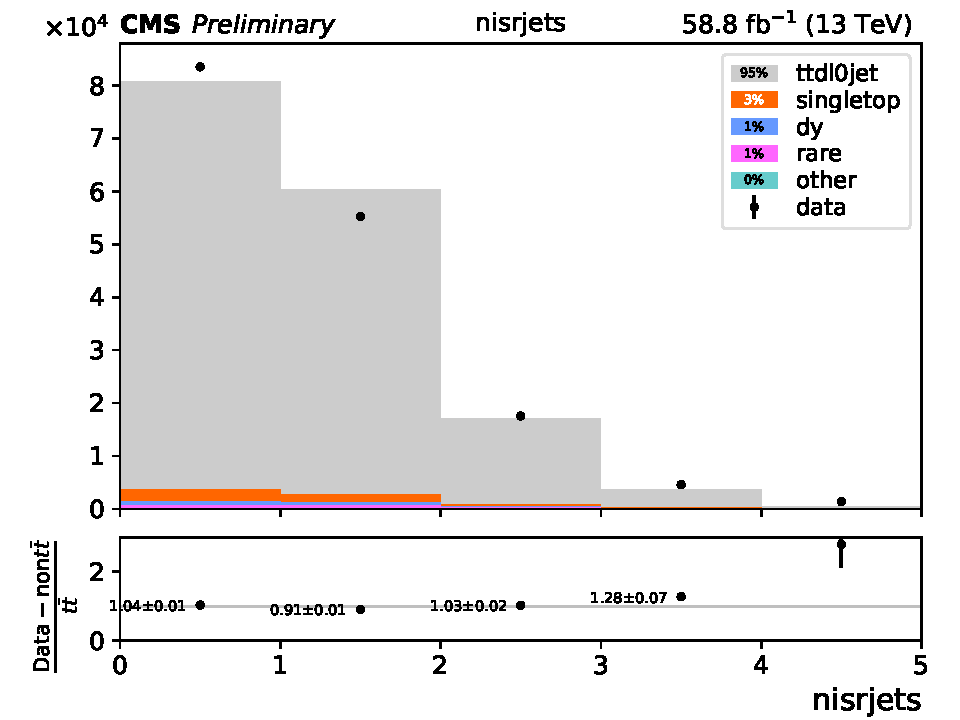
\includegraphics[width=0.48\textwidth]{figs/ftan/isr/y2018_isrrw_nisrjets0.pdf}
  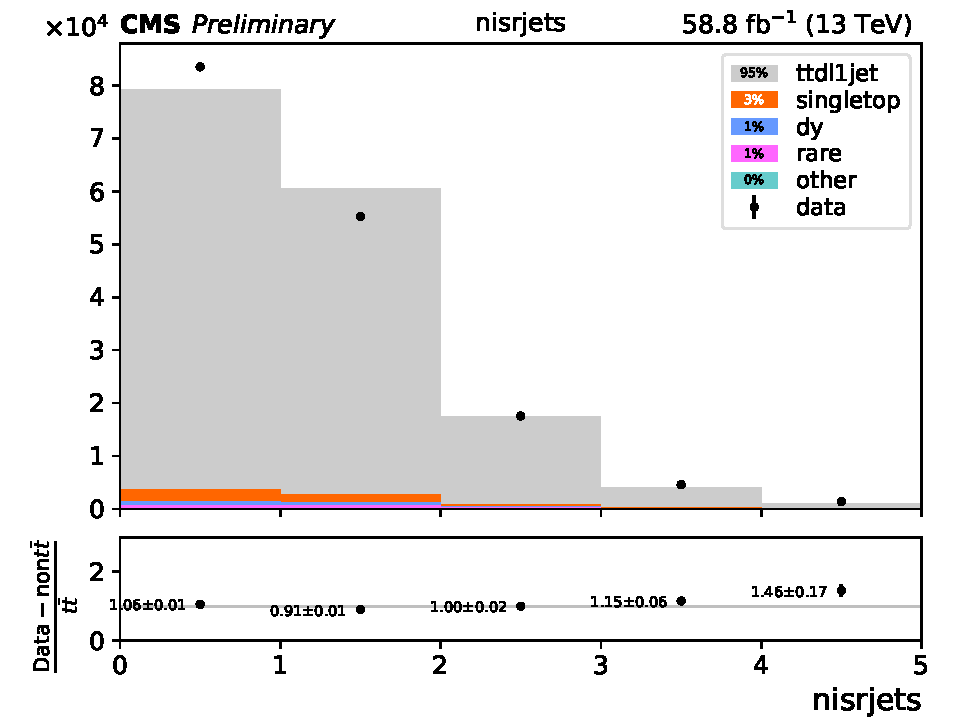
\includegraphics[width=0.48\textwidth]{figs/ftan/isr/y2018_isrrw_nisrjets1.pdf}
  \caption{
      Distribution of the number of light jets in a dilepton \ttbar sample with 0
      additional partons (left) or 1 additional parton (right) for 2017 data
      (top) and 2018 data (bottom) compared to their respective MC samples.
      In the case of 0 additional partons, the reweighing factor in the last bin
      is taken instead from the previous bin.
  }
  \label{fig:isrweight2}
  \end{figure}

\begin{figure}[h!]
\centering
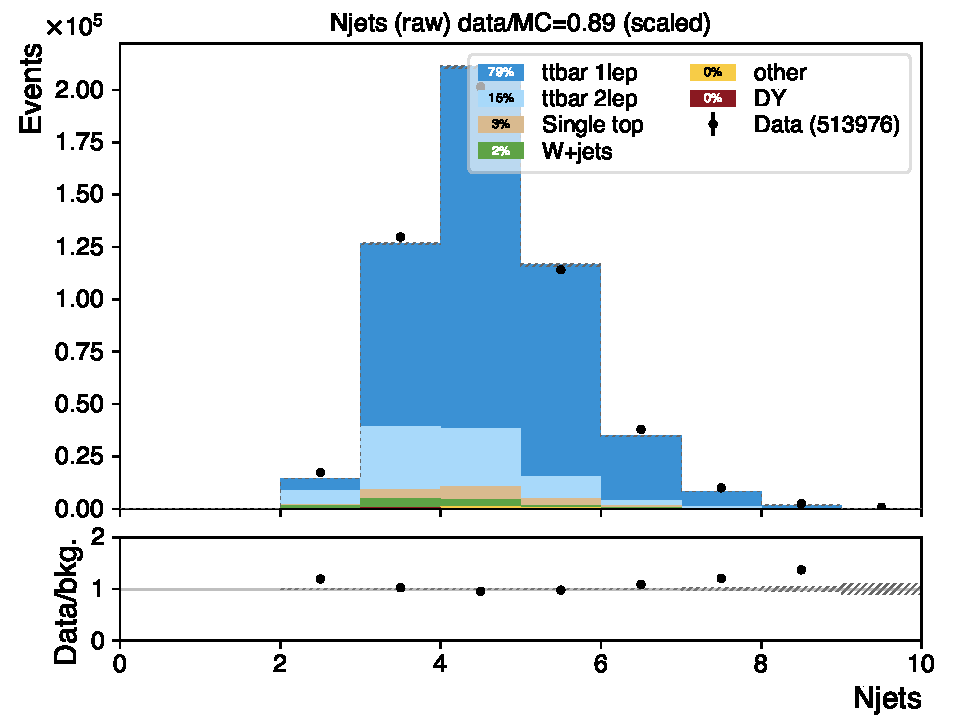
\includegraphics[width=0.70\textwidth]{figs/ftan/isr/njets_raw.pdf} \\
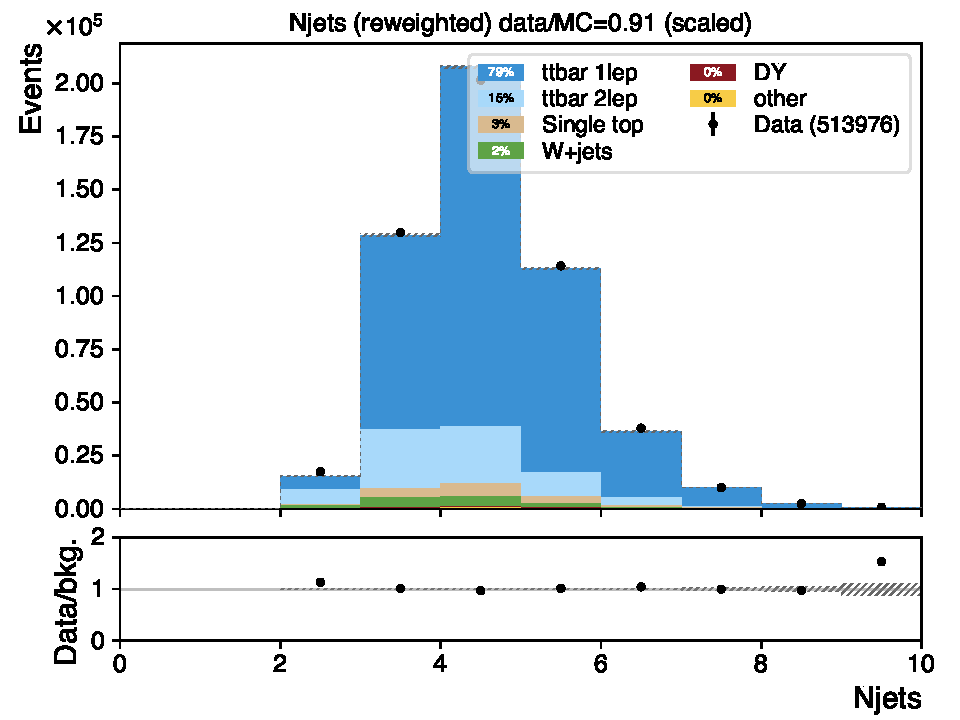
\includegraphics[width=0.70\textwidth]{figs/ftan/isr/njets_corr.pdf}
\caption{
    Jet multiplicity distribution for 2018 data/MC before (top) and after (bottom)
    applying the 2018-derived reweighting factors. The ``other'' category includes
    leading diboson, \ttW, and \ttZ contributions.
}
\label{fig:isrweightsyst}
\end{figure}


\FloatBarrier

\section{Control regions}

In this section we describe the control regions (CRs) used to validate our background
prediction methods with data for the main kinematic variables
we use in defining our SRs: $\HT$, $\ptmiss$, $\MTmin$,
$\Njets$, $\Nbjets$, and for the case of the \smft analysis, the input variables
to the event-level BDT. In general, we observe good agreement across these CRs.


\subsection{SUSY: OS events}

In this CR, the same requirements on $\HT$, $\ptmiss$ and $\Njets$ as in the
inclusive SUSY analysis baseline selection are applied, except we require two
OS tight leptons. This CR thus coincides with the application region usd for
the data-driven charge flip background estimate. Distributions are shown in
Fig.~\ref{fig:OSBaselineMET}. The variables are plotted again with a
selection that relaxes the baseline $\ptmiss$ cut in
Fig.~\ref{fig:OSBaselineNoMET}.

\begin{figure}[!htb]
\centering
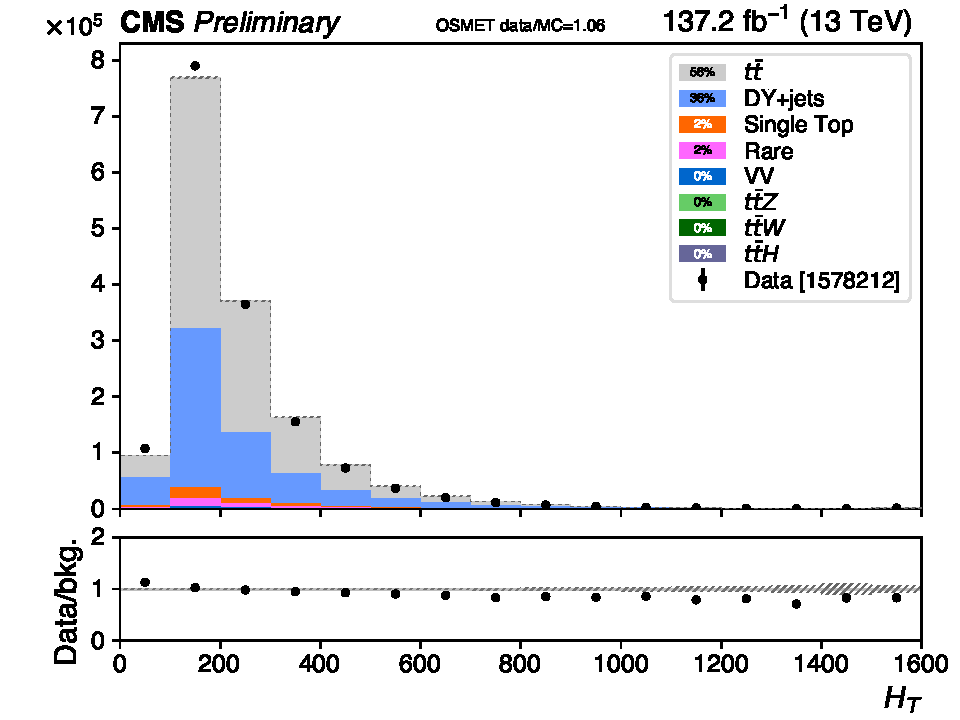
\includegraphics[width=0.45\linewidth]{figs/ssan/cr/run2_osmet_ht_in.pdf} 
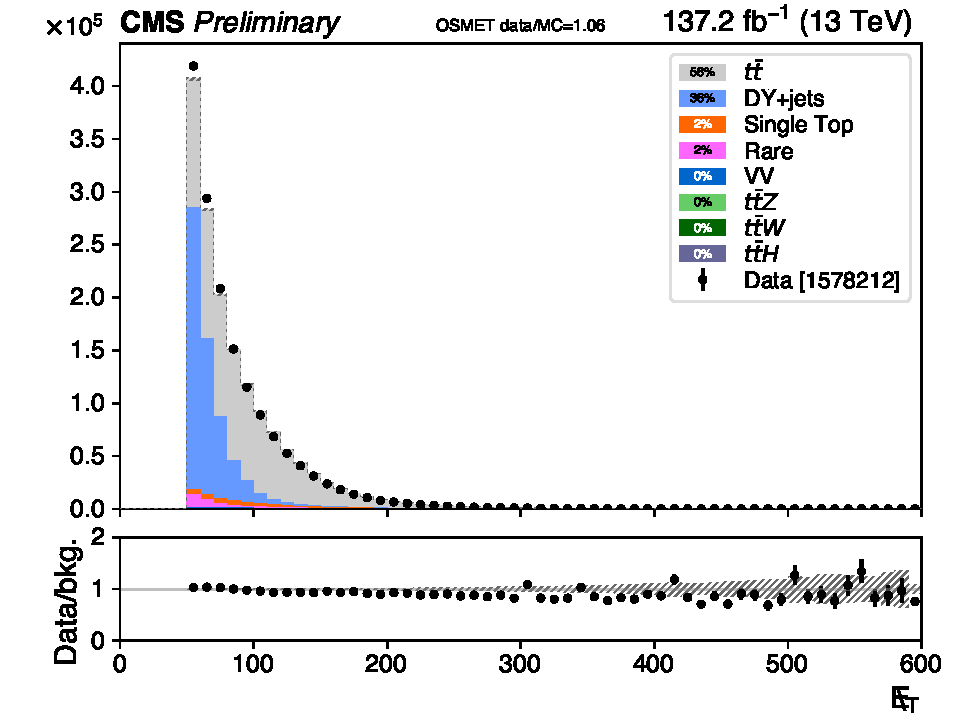
\includegraphics[width=0.45\linewidth]{figs/ssan/cr/run2_osmet_met_in.pdf} 
\includegraphics[width=0.45\linewidth]{figs/ssan/cr/run2_osmet_mtmin_in.pdf}
\includegraphics[width=0.45\linewidth]{figs/ssan/cr/run2_osmet_njets_in.pdf} 
\includegraphics[width=0.45\linewidth]{figs/ssan/cr/run2_osmet_nbtags_in.pdf}
\caption{ Data to simulation comparisons. From left to right  and top to bottom,
the $\HT$, $\ptmiss$, $\MTmin$, $\Njets$, $\Nbjets$ distributions are
shown for the OS CR.}
\label{fig:OSBaselineMET}
\end{figure}



\begin{figure}[!htb]
\centering
\includegraphics[width=0.45\linewidth]{figs/ssan/cr/run2_osnomet_ht_in.pdf} 
\includegraphics[width=0.45\linewidth]{figs/ssan/cr/run2_osnomet_met_in.pdf} 
\includegraphics[width=0.45\linewidth]{figs/ssan/cr/run2_osnomet_mtmin_in.pdf}
\includegraphics[width=0.45\linewidth]{figs/ssan/cr/run2_osnomet_njets_in.pdf} 
\includegraphics[width=0.45\linewidth]{figs/ssan/cr/run2_osnomet_nbtags_in.pdf}
\caption{ Data to simulation comparisons. From left to right  and top to bottom,
the $\HT$, $\ptmiss$, $\MTmin$, $\Njets$, $\Nbjets$ distributions are
shown for the OS CR, relaxing the $\ptmiss$ cut.}
\label{fig:OSBaselineNoMET}
\end{figure}

\FloatBarrier

\subsection{SUSY: SS tight-loose events}

This tight-loose (TL) CR has selections coinciding with the inclusive SUSY
analysis baseline selection except with one tight lepton and one lepton
failing the tight requirements (but passing the loose requirements). This CR
roughly corresponds to the application region used for the nonprompt lepton
background estimate. The variables are plotted again with a selection that
relaxes the baseline $\ptmiss$ cut in Fig.~\ref{fig:TLBaselineNoMET}.



\begin{figure}[!htb]
\centering
\includegraphics[width=0.45\linewidth]{figs/ssan/cr/run2_tlmet_ht_in.pdf} 
\includegraphics[width=0.45\linewidth]{figs/ssan/cr/run2_tlmet_met_in.pdf} 
\includegraphics[width=0.45\linewidth]{figs/ssan/cr/run2_tlmet_mtmin_in.pdf}
\includegraphics[width=0.45\linewidth]{figs/ssan/cr/run2_tlmet_njets_in.pdf} 
\includegraphics[width=0.45\linewidth]{figs/ssan/cr/run2_tlmet_nbtags_in.pdf}
\caption{ Data to simulation comparisons. From left to right  and top to bottom,
the $\HT$, $\ptmiss$, $\MTmin$, $\Njets$, $\Nbjets$ distributions are
shown for the TL CR.}
\label{fig:TLBaselineMET}
\end{figure}



\begin{figure}[!htb]
\centering
\includegraphics[width=0.45\linewidth]{figs/ssan/cr/run2_tlnomet_ht_in.pdf} 
\includegraphics[width=0.45\linewidth]{figs/ssan/cr/run2_tlnomet_met_in.pdf} 
\includegraphics[width=0.45\linewidth]{figs/ssan/cr/run2_tlnomet_mtmin_in.pdf}
\includegraphics[width=0.45\linewidth]{figs/ssan/cr/run2_tlnomet_njets_in.pdf} 
\includegraphics[width=0.45\linewidth]{figs/ssan/cr/run2_tlnomet_nbtags_in.pdf}
\caption{ Data to simulation comparisons. From left to right  and top to bottom,
the $\HT$, $\ptmiss$, $\MTmin$, $\Njets$, $\Nbjets$ distributions are
shown for the TL CR, relaxing the $\ptmiss$ cut.}
\label{fig:TLBaselineNoMET}
\end{figure}

\FloatBarrier

\subsection{SUSY: Low $\ptmiss$ on-Z multi-lepton events}\label{LowMetOnZCR}

In this CR, the same requirements on $\HT$
and $\Njets$ as in the inclusive SUSY analysis baseline selection are applied,
and we also apply the same requirements
as for the on-Z multi-lepton kinematic regions, except the $\ptmiss$ cut is inverted, 
becoming $\ptmiss < 50 \GeV$.
Distributions are shown in Fig.~\ref{fig:MLLowMetBaseline}.

\begin{figure}[!htb]
\centering
\includegraphics[width=0.45\linewidth]{figs/ssan/cr/run2_mlonz_ht_in.pdf} 
\includegraphics[width=0.45\linewidth]{figs/ssan/cr/run2_mlonz_met_in.pdf} 
\includegraphics[width=0.45\linewidth]{figs/ssan/cr/run2_mlonz_mtmin_in.pdf}
\includegraphics[width=0.45\linewidth]{figs/ssan/cr/run2_mlonz_njets_in.pdf} 
\includegraphics[width=0.45\linewidth]{figs/ssan/cr/run2_mlonz_nbtags_in.pdf}
\caption{ Data to simulation comparisons. From left to right  and top to bottom,
the $\HT$, $\ptmiss$, $\MTmin$, $\Njets$, $\Nbjets$ distributions are
shown for the low $\ptmiss$ on-Z multi-lepton region}
\label{fig:MLLowMetBaseline}
\end{figure}


\FloatBarrier

\subsection{SUSY: Low $\ptmiss$ SS events}\label{LowMetSS}

This CR is the low-$\HT$ version of the low \ptmiss inclusive SUSY analysis SRs, so selections
are identical except we require $\HT<300 \GeV$ to be orthogonal to the SR definitions.
Distributions are shown in Fig.~\ref{fig:LowMetSSBaseline}.

\begin{figure}[!htb]
\centering
\includegraphics[width=0.45\linewidth]{figs/ssan/cr/run2_lowmetlowht_ht_in.pdf} 
\includegraphics[width=0.45\linewidth]{figs/ssan/cr/run2_lowmetlowht_met_in.pdf} 
\includegraphics[width=0.45\linewidth]{figs/ssan/cr/run2_lowmetlowht_mtmin_in.pdf}
\includegraphics[width=0.45\linewidth]{figs/ssan/cr/run2_lowmetlowht_njets_in.pdf} 
\includegraphics[width=0.45\linewidth]{figs/ssan/cr/run2_lowmetlowht_nbtags_in.pdf}
\caption{ Data to simulation comparisons. From left to right  and top to bottom,
the $\HT$, $\ptmiss$, $\MTmin$, $\Njets$, $\Nbjets$ distributions are
shown for the low $\ptmiss$ CR}
\label{fig:LowMetSSBaseline}
\end{figure}


\FloatBarrier

\subsection{\smft: OS events}\label{sec:OSCR}

In this CR, the same requirements on $\HT$, $\ptmiss$
and $\Njets$ as in the \smft analysis baseline selection are applied,
but we require two OS tight
leptons and we remove the $\PZ/\gamma^*$ veto. This CR
coincides with the application region we use for the data-driven
method to estimate the charge flips background.
Distributions are shown in Fig.~\ref{fig:OSBaselineRun2} for the main variables, 
and Fig.~\ref{fig:OSBaselineExtraRun2} for additional variables used in the BDT. 

\begin{figure}[!htb]
\centering
\includegraphics[width=0.45\linewidth]{figs/ftan/cr/run2_os_ht_in.pdf} 
\includegraphics[width=0.45\linewidth]{figs/ftan/cr/run2_os_met_in.pdf}  
\includegraphics[width=0.45\linewidth]{figs/ftan/cr/run2_os_njets_in.pdf}
\includegraphics[width=0.45\linewidth]{figs/ftan/cr/run2_os_nbtags_in.pdf} 
\includegraphics[width=0.45\linewidth]{figs/ftan/cr/run2_os_type_in.pdf} 
\includegraphics[width=0.45\linewidth]{figs/ftan/cr/run2_os_eventbdt_in.pdf} 
\caption{ Data to simulation comparisons. From left top to right bottom
  the $\HT$, $\ptmiss$, $\Njets$, $\Nbjets$, lepton flavor and raw BDT discriminant distributions are
shown for the opposite-sign dilepton baseline region. Shaded band shows MC stat uncertainty,
except in the case of the discriminator distribution, where it has been added in quadrature with
    scale, btag, JEC, and JER variations}
\label{fig:OSBaselineRun2}
\end{figure}


\begin{figure}[!htb]
\centering
\includegraphics[width=0.32\linewidth]{figs/ftan/cr/run2_os_htb_in.pdf} 
\includegraphics[width=0.32\linewidth]{figs/ftan/cr/run2_os_nlb40_in.pdf} 
\includegraphics[width=0.32\linewidth]{figs/ftan/cr/run2_os_ntb40_in.pdf}
\includegraphics[width=0.32\linewidth]{figs/ftan/cr/run2_os_dphil1l2_in.pdf} 
\includegraphics[width=0.32\linewidth]{figs/ftan/cr/run2_os_detal1l2_in.pdf} 
\includegraphics[width=0.32\linewidth]{figs/ftan/cr/run2_os_pt1_in.pdf}
\includegraphics[width=0.32\linewidth]{figs/ftan/cr/run2_os_pt2_in.pdf} 
\includegraphics[width=0.32\linewidth]{figs/ftan/cr/run2_os_q1_in.pdf}
\includegraphics[width=0.32\linewidth]{figs/ftan/cr/run2_os_ml1j1_in.pdf}
\includegraphics[width=0.32\linewidth]{figs/ftan/cr/run2_os_maxmjoverpt_in.pdf} 
\includegraphics[width=0.32\linewidth]{figs/ftan/cr/run2_os_ptj1_in.pdf} 
\includegraphics[width=0.32\linewidth]{figs/ftan/cr/run2_os_ptj6_in.pdf}
\includegraphics[width=0.32\linewidth]{figs/ftan/cr/run2_os_ptj7_in.pdf}
\includegraphics[width=0.32\linewidth]{figs/ftan/cr/run2_os_ptj8_in.pdf}
\caption{ Data to simulation comparisons for the additional variables used by the BDT. From left top to right bottom,
$H_T^b$, $\Nbjets^\text{loose}$, $\Nbjets^\text{tight}$, $\Delta \phi(\ell_{1},\ell_2)$, 
$\Delta \eta(\ell_{1},\ell_{2})$, $p_T(\ell_1)$, $p_T(\ell_2)$, $p_T(\ell_3)$,
    $q_1$, $m(\ell_1,j_1)$, max($m(j)/p_T(j)$) and the \pt for jets 1, 6, 7, and 8;
shown for the opposite-sign dilepton baseline region. }
\label{fig:OSBaselineExtraRun2}
\end{figure}

\FloatBarrier
  
\subsection{\smft: SS tight-loose events}\label{sec:TLCR}

In this CR, the same requirements on $\HT$, $\ptmiss$
and $\Njets$ as in the inclusive \smft analysisbaseline selection are applied,
but we require one tight lepton and
one same-sign lepton failing the tight requirement. This CR is
enriched in events with one fake lepton, and roughly corresponds to the application region for 
nonprompt lepton background estimate.
Distributions are shown in Fig.~\ref{fig:TightFailBaselineRun2} for the main variables, 
and Fig.~\ref{fig:TightFailBaselineExtraRun2} for additional variables used in the BDT. 
While there is an overall underestimate, there does not seem to be large trends in the main
kinematic variables. Since this background is predicted from data, this understimate is
not an issue with the analysis strategy.

\begin{figure}[!htb]
\centering
\includegraphics[width=0.45\linewidth]{figs/ftan/cr/run2_tl_ht_in.pdf} 
\includegraphics[width=0.45\linewidth]{figs/ftan/cr/run2_tl_met_in.pdf}  
\includegraphics[width=0.45\linewidth]{figs/ftan/cr/run2_tl_njets_in.pdf}
\includegraphics[width=0.45\linewidth]{figs/ftan/cr/run2_tl_nbtags_in.pdf} 
\includegraphics[width=0.45\linewidth]{figs/ftan/cr/run2_tl_type_in.pdf} 
\includegraphics[width=0.45\linewidth]{figs/ftan/cr/run2_tl_eventbdt_in.pdf} 
\caption{ Data to simulation comparisons. From left top to right bottom
  the $\HT$, $\ptmiss$, $\Njets$, $\Nbjets$, lepton flavor and raw BDT discriminant distributions are
shown for the same-sign tight+fail dilepton baseline region. Shaded band shows MC stat uncertainty,
except in the case of the discriminator distribution, where it has been added in quadrature with
    scale, btag, JEC, and JER variations}
\label{fig:TightFailBaselineRun2}
\end{figure}


\begin{figure}[!htb]
\centering
\includegraphics[width=0.32\linewidth]{figs/ftan/cr/run2_tl_htb_in.pdf} 
\includegraphics[width=0.32\linewidth]{figs/ftan/cr/run2_tl_nlb40_in.pdf} 
\includegraphics[width=0.32\linewidth]{figs/ftan/cr/run2_tl_ntb40_in.pdf}
\includegraphics[width=0.32\linewidth]{figs/ftan/cr/run2_tl_dphil1l2_in.pdf} 
\includegraphics[width=0.32\linewidth]{figs/ftan/cr/run2_tl_detal1l2_in.pdf} 
\includegraphics[width=0.32\linewidth]{figs/ftan/cr/run2_tl_pt1_in.pdf}
\includegraphics[width=0.32\linewidth]{figs/ftan/cr/run2_tl_pt2_in.pdf}
\includegraphics[width=0.32\linewidth]{figs/ftan/cr/run2_tl_pt3_in.pdf} 
\includegraphics[width=0.32\linewidth]{figs/ftan/cr/run2_tl_q1_in.pdf}
\includegraphics[width=0.32\linewidth]{figs/ftan/cr/run2_tl_ml1j1_in.pdf}
\includegraphics[width=0.32\linewidth]{figs/ftan/cr/run2_tl_maxmjoverpt_in.pdf} 
\includegraphics[width=0.32\linewidth]{figs/ftan/cr/run2_tl_ptj1_in.pdf} 
\includegraphics[width=0.32\linewidth]{figs/ftan/cr/run2_tl_ptj6_in.pdf}
\includegraphics[width=0.32\linewidth]{figs/ftan/cr/run2_tl_ptj7_in.pdf}
\includegraphics[width=0.32\linewidth]{figs/ftan/cr/run2_tl_ptj8_in.pdf}
\caption{ Data to simulation comparisons for the additional variables used by the BDT. From left top to right bottom,
    $H_{T}^b$, $\Nbjets^\text{loose}$, $\Nbjets^\text{tight}$, $\Delta \phi(\ell_{1},\ell_2)$, 
$\Delta \eta(\ell_{1},\ell_{2})$, $p_T(\ell_1)$, $p_T(\ell_2)$, $p_T(\ell_3)$,
    $q_1$, $m(\ell_1,j_1)$, max($m(j)/p_T(j)$) and the \pt for jets 1, 6, 7, and 8;
shown for the same-sign tight+fail dilepton baseline region. }
\label{fig:TightFailBaselineExtraRun2}
\end{figure}

\FloatBarrier

\subsection{\smft: Fake-enriched events}\label{sec:FECR}

In this CR, the same requirements on $\HT$, $\ptmiss$
and $\Njets$ as in the inclusive \smft analysis baseline selection are applied,
except we relax the $\HT$ requirement
and require $\Nbjets=1$.
This region has a significant nonprompt lepton component and allows us to check the
overall closure of the method in data. In the plots, the fake background is data-driven.
Distributions are shown in Figs.~\ref{fig:FakeEnrichedBaselineRun2}.
As written on the plots, overall data/MC normalization factor in this region is 1.06. 
If fakes are entirely responsible for this discrepancy,
and given that fakes constitute half of the background, this
represents a 12\% normalization increase of fakes, well within the 30\% normalization
systematic uncertainty which we take on this process.

\begin{figure}[!htb]
\centering
\includegraphics[width=0.45\linewidth]{figs/ftan/cr/run2_htnb1_ht_in.pdf} 
\includegraphics[width=0.45\linewidth]{figs/ftan/cr/run2_htnb1_met_in.pdf}  
\includegraphics[width=0.45\linewidth]{figs/ftan/cr/run2_htnb1_njets_in.pdf}
\includegraphics[width=0.45\linewidth]{figs/ftan/cr/run2_htnb1_nbtags_in.pdf} 
\includegraphics[width=0.45\linewidth]{figs/ftan/cr/run2_htnb1_type_in.pdf} 
\caption{ Data to simulation comparisons. From left top to right bottom
  the $\HT$, $\ptmiss$, $\Njets$, $\Nbjets$, lepton flavor and raw BDT discriminant distributions are
shown for the same-sign dilepton region with $\Nbjets=1$, $\Njets\geq 2$, $\ptmiss\geq50$. Shaded band shows MC stat uncertainty.
    }
\label{fig:FakeEnrichedBaselineRun2}
\end{figure}

\FloatBarrier

\section{Systematic uncertainties}

Sources of systematic uncertainty, many of which
are associated with corrections and calibrations discussed previously,
are summarized in Tables~\ref{tab:SUSYsystSummary} and \ref{tab:FTsystSummary},
for the inclusive SUSY analysis and \smft analysis, respectively.

Uncertainties for processes
are considered on the process normalization (number of events),
and shape (distribution of events across the SRs).
Experimental uncertainties in normalization and shape are treated as
fully correlated among the SRs for all signal and background processes.

For the \smft analysis, the \tttt signal has an unconstrained normalization uncertainty
in order to measure its cross section. In this analysis, the largest
sources of uncertainty, on the basis of what impacts the measurement of \tttt the most,
are jet-related, and dominated by the correction that reweights
the extra \cPqb contribution. However, to put these uncertainties into perspective,
less than approximately a quarter of the precision of the \tttt measurement
comes from systematic uncertainties. The remaining amount comes from statistics.
That is, the \smft measurement precision primarily benefits from increased luminosity.

\begin{table}[!hbtp]
  \centering
{\renewcommand{\arraystretch}{1.2}
  \begin{tabular}{lcc}
      \hline
  Source          & Uncertainty (\%) & Correlated \\
  \hline
  Integrated luminosity & 2.3--2.5 &  \\
  Lepton selection & 2--10 & \\
  Trigger efficiency & 2--7  & \\
  Pileup & 0--6  &\\
  Jet energy scale & 1--15 &\\
  $\cPqb$ tagging & 1--10  &\\
  Simulated sample size & 1--20 & \\
  \hline
  Scale and PDF variations & 10--20 &Yes\\
  Theoretical background cross sections & 30--50& Yes\\
  \hline
  Nonprompt leptons & 30 & Yes \\
  Charge misidentification & 20  & \\
  \nisrjet & 1--30  & \\
      \hline
  \end{tabular}}
      \caption{
     Summary of the sources of systematic uncertainty and their effect on the yields of different processes in the SRs.
      The first two groups list experimental and theoretical uncertainties assigned to processes estimated using simulation,
      while the last group lists uncertainties assigned to processes whose yield is estimated from the data.
      The uncertainties in the first group also apply to signal samples.
      Reported values are representative for the most relevant signal regions.
        The last column indicates if an uncertainty source is treated as 
        fully uncorrelated across the three years of data taking.
      }
      \label{tab:SUSYsystSummary}
  \end{table}

  \begin{table}[!hbt]
    \centering
{\renewcommand{\arraystretch}{1.2}
        \begin{tabular}{lccc}
        \hline
        &                  & Impact on \\
        Source & Uncertainty (\%) & $\sigma(\ttbar\ttbar)$ (\%) & Correlated \\
    \hline
        Integrated luminosity                                & 2.3--2.5         & 2 & \\
        Pileup                                               & 0--5             & 1 & \\
        Trigger efficiency                                   & 2--7             & 2 & \\
        Lepton selection                                     & 2--10            & 2 & \\
        Jet energy scale                                     & 1--15            & 9 & \\
        Jet energy resolution                                & 1--10            & 6 & \\
        $\cPqb$ tagging                                      & 1--15            & 6 & \\
        Size of simulated sample                             & 1--25            & $<$1 & \\
        Scale and PDF variations                   & 10--15           & 2 & Yes \\
        ISR/FSR (signal)                           & 5--15            & 2 & Yes \\
        \hline
        $\ttbar \PH$ (normalization)               & 25               & 5 & Yes \\
        Rare, \Xgamma, \ttVV (norm.)   & 11--20            & $<$1 & Yes \\
        $\ttbar \PZ$, $\ttbar \PW$ (norm.)         & 40               & 3--4 & Yes \\
        Charge misidentification                   & 20               & $<$1 & Yes \\
        Nonprompt leptons                        & 30--60           & 3 & Yes \\
        $N_{\text{jets}}^{\mathrm{ISR/FSR}}$                    & 1--30             & 2 & \\
        $\sigma({\ttbar\bbbar})/\sigma({\ttbar jj})$ & 35               & 11 & Yes \\
        \hline
    \end{tabular}}
        \caption{
       Summary of the sources of uncertainty, their values, and their impact, defined as the relative change of the
       measurement of $\sigma(\ttbar\ttbar)$ induced by one-standard-deviation variations corresponding to each uncertainty source considered separately.
        The first group lists experimental and theoretical uncertainties
        in simulated signal and background processes.
        The second group lists normalization uncertainties in the estimated backgrounds.
        The last column indicates if an uncertainty source is treated as 
        fully uncorrelated across the three years of data taking.
        }
        \label{tab:FTsystSummary}
    \end{table}

\FloatBarrier
